\section{Introduction}

Sections of this chapter appear in a manuscript submitted to Springer link as part of the International Conference on Computational 
Science (ICCS) 2025 in the Computing and Data Science for Materials Discovery and Design track, submission number 259 and is
% [author and/or editor(s) of contribution], [volume and/or contribution title], [year of publication], [publisher (as it appears on our copyright page)] \
reproduced with permission of Palgrave Springer Nature. 

Emulsions can adopt a variety of microstructures depending on fluid volume fractions and the affinity of stabilizing agents for each phase. Among these, bicontinuous 
interfacially jammed emulsion gels (bijels) are characterized by a tortuous, co-continuous network of immiscible fluid domains stabilized by colloidal particles. This 
unique architecture lends itself to numerous advanced applications, including membrane fabrication, catalyst supports, battery electrodes, and pharmaceutical delivery 
systems. Bijels form through the arrest of spinodal decomposition in partially miscible fluid mixtures: as phase separation proceeds, the interface sweeps through the 
system, adsorbing particles until the interfacial area becomes saturated, resulting in jamming. Microstructural features such as domain size, continuity, and interfacial 
curvature critically influence material performance, affecting properties like mass transport, mechanical stability, and surface reactivity. Since their discovery via 
simulation and subsequent experimental realization, research on bijels has expanded significantly, exploring diverse synthesis conditions and scalable processing methods.

The functional properties of bijels are inherently linked to their internal structure. For instance, lower tortuosities in the direction of ion transport yield improved 
charge rates and cycling stability in battery electrodes \cite{ebner_tortuosity_2014, samdani_bicontinuous_2017}. In liquid-liquid extraction, the characteristic pore 
lengthscale determines molecular selectivity \cite{khan_nanostructured_2022}, while in pharmaceutical applications, domain size influences drug release rates and cellular 
behavior \cite{vanoli_bijels_2022, thorson_bijel-templated_2019}. Given the sensitivity of these properties to microstructural characteristics, the ability to dynamically 
modify the morphology of bijels presents a promising strategy to adapt their behavior in situ for targeted performance.

Stimuli-responsive emulsions have garnered increasing interest for applications requiring dynamic control over material properties, including enhanced oil recovery, reaction 
separation, and therapeutic delivery \cite{tham_magnetophoresis_2021, cui_stabilizing_2013, rozynek_opening_2019, lu_controllable_2020}. These systems operate by using 
external stimuli to alter interfacial configurations, enabling modulation of permeability, interfacial area, and morphology. For example, in emulsions stabilized by 
spherical particles, electric fields can induce droplet deformation via particle unjamming and migration before re-establishing interfacial jamming \cite{cui_stabilizing_2013}. 
Among various external stimuli, magnetic fields are particularly attractive due to their remote addressability, material compatibility, and bio-relevance. 
Core-shell ferrite-hydroxyapatite nanorods, for instance, exhibit reversible morphological changes depending on initial particle orientation and field direction 
\cite{nakayama_stimuli-responsive_2018}. In magnetically stabilized Pickering emulsions, magnetophoresis has been shown to drive particle migration and interfacial 
distortion or collapse \cite{tham_magnetophoresis_2021, yang_rapid_2020, misra_magnetic_2020}. Notably, Karthikeyan and Schiller demonstrated that magnetic fields applied 
during bijel formation can bias domain coarsening, producing anisotropic microstructures via orientation-specific jamming \cite{karthikeyan_formation_2024}. However, the 
structural response of bijels to magnetic fields after formation remains poorly understood.

This study investigates the post-formation structural response of bijels stabilized by ellipsoidal magnetic particles under the influence of externally applied magnetic fields. 
Using a hybrid Lattice Boltzmann Method coupled with Molecular Dynamics, we simulate the formation and evolution of bijel structures stabilized by rod-like particles modeled as 
magnetic dipoles. We find that increasing the applied magnetic field after formation induces significant microstructural changes, including increased domain anisotropy and 
coarsening, up to a saturation threshold. In contrast, decreasing or removing the magnetic field results in minimal morphological change, suggesting a strong hysteresis effect. 
Analysis reveals that particle unjamming, reorientation at the interface, and subsequent re-jamming are responsible for these structural transformations.

To understand the saturation behavior, we applied magnetic fields of varying strength to bijel templates formed under increasing initial field conditions. We observed that 
a greater initial nematic order parameter negatively correlated with the extent of microstructure change. Finally, switching off the magnetic field in pre-aligned bijels had little 
impact on the microstructure, indicating that the jammed interfacial network prevents reversal of anisotropic features. These findings underscore the importance of processing 
history and demonstrate how magnetic field manipulation, in combination with anisotropic particle stabilization, enables tunable, on-demand microstructure control in bijels, 
offering new capabilities for adaptive material design.

\section{Results}\label{sec:results_p2}
\subsection{Hysteresis curve}
\label{section:hysteresis_curve}

Bijels have proposed applications as soft-matter-based material templates, drug delivery vectors, and separation systems. In all cases, material performance is 
tightly coupled to the internal microstructure of the bijel template. Applications that benefit from adaptive permeability or structural tunability would be 
enhanced by the ability to reversibly modulate microstructure in situ. This section explores whether magnetically responsive bijels can undergo reversible 
structural changes upon repeated application and removal of an external magnetic field.

We begin by analyzing bijels stabilized by prolate ellipsoidal particles at a particle volume fraction of \(\phi_p = 0.1\). This system is selected due to the 
similar qualitative response mechanisms observed for both prolate and oblate geometries in preliminary simulations (Aim 1), with prolate particles chosen here 
for their greater experimental accessibility. The bijel is initially formed without a magnetic field. After equilibration, a static magnetic field is applied 
in the \(z\)-direction and incrementally increased: \(\bar{B}_z = 0 \rightarrow 0.2 \rightarrow 0.5 \rightarrow 1\). This is followed by a symmetric 
decrement: \(\bar{B}_z = 1 \rightarrow 0.5 \rightarrow 0.2 \rightarrow 0\). At each step, the system is allowed to evolve to a new equilibrium, defined as
the plateauing of the length scale obtained from the domain size, \(L\), computed from the first moment of the spherically averaged structure factor.
\cite{kendon_3d_1999,kendon_inertial_2001} The structure factor is calculated from the density fields as,

%
\begin{equation}
S(\vec{k},t) = \tilde{\phi}(\vec{k},t)\tilde{\phi}(-\vec{k},t) .
\end{equation}
%
where \(\tilde{\phi}(\vec{k},t)\) is the Fourier
transform of the order parameter fluctuations
\(\phi(\vec{x},t)-\left\langle\phi\right\rangle\). Spherical averaging is 
done by averaging the values of the structure factor where $k = |\vec{k}|$ is in
the same bin, defined as

%
\begin{equation}
S(k,t) = \frac{1}{n_k} \sum_{k-\frac{\Delta}{2}<k<k+\frac{\Delta}{2}} \tilde{\phi}(\vec{k},t)\tilde{\phi}(-\vec{k},t) ,
\end{equation}

The lengthscale is then defined as

\begin{equation}
    L = \frac{2 \pi}{\frac{ \sum_k S(k, t)k }{\sum_k S(k, t)}}
\end{equation}

The hysteresis behavior is shown in Figure~\ref{fig:hysteresis_curve}, which plots the normalized domain size \(L/R\) as a function of the applied magnetic 
field at the end of the equilibration step.

\begin{figure} 
    \centering 
    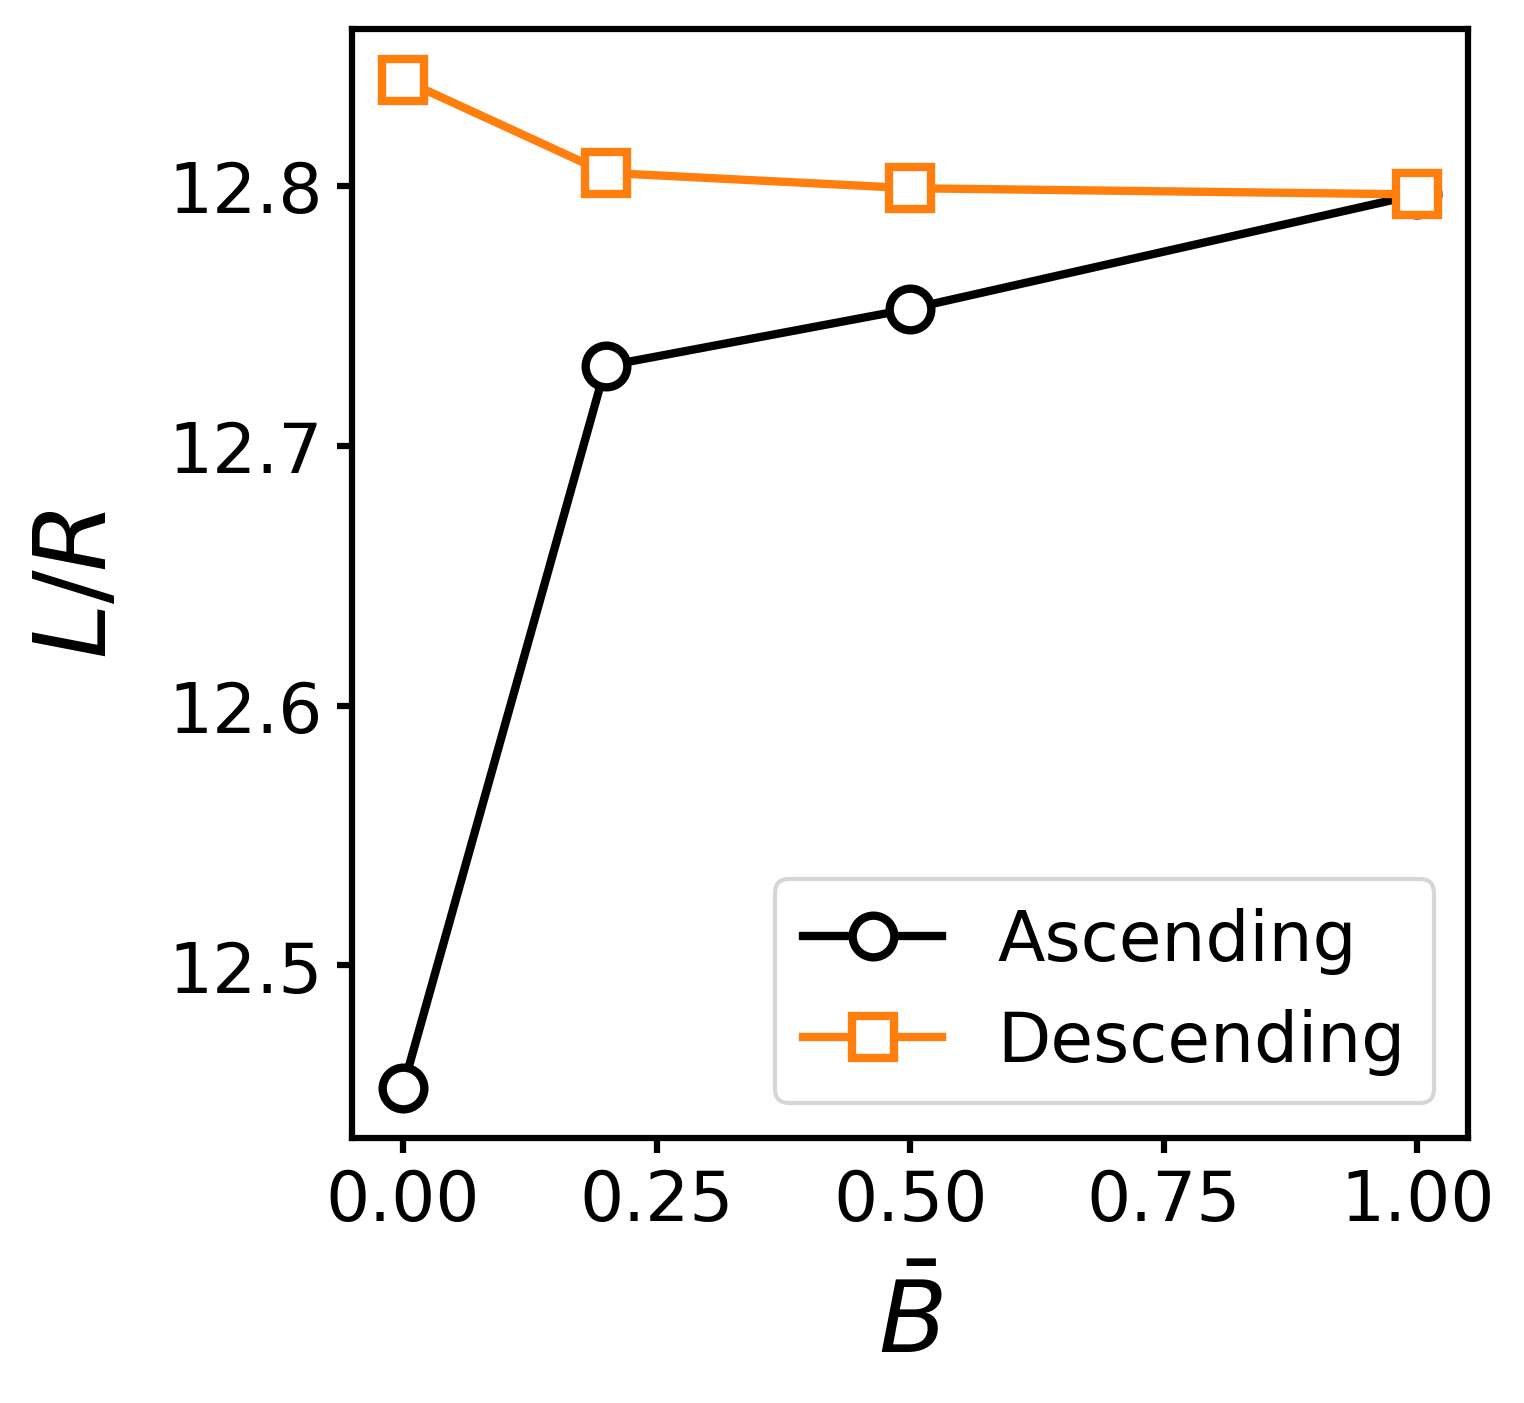
\includegraphics[scale=0.5]{../figures/results/paper2/hysteresis_curve.png} 
    \caption{Plot of the hysteresis curve of a bijel stabilized by magnetically responsive prolate particles. We observe that the domain size increases as we 
    increase the applied magnetic field strength. However, upon decrease of the applied field strength the microstructure does not return to its previous value,
    demonstrating microstructure hysteresis.} 
    \label{fig:hysteresis_curve} 
\end{figure}

The hysteresis behavior is shown in Figure~\ref{fig:hysteresis_curve} demonstrates that as the field is increased, domain size increases, indicating coarsening 
of the fluid domains in the bijel. Karthikeyan and Schiller showed that application of magnetic fields cause reordering of particles at interfaces towards the
direction of the applied field, making the particle monolayer have nematic ordering. In the case of already formed bijels,
this reorientation likely reduces the interface area stabilized, facilitating local unjamming and domain growth. In contrast, when the field strength is reduced, 
the domain size does not revert to its original value, suggesting that the microstructure remains kinetically arrested in the coarsened configuration. This 
irreversibility confirms a hysteretic response of the bijel structure to magnetic field cycling.

A similar phenomenon has been reported by Cui et al.~\cite{cui_stabilizing_2013} in studies of particle-stabilized emulsions subjected to electric fields, 
where spherical particles unjammed and subsequently rejammed in a new configuration, resulting in anisotropic droplet deformation. Our results extend this 
concept to jammed, bicontinuous systems stabilized by anisotropic particles. Notably, Figure~\ref{fig:hysteresis_curve} also shows that the degree of 
structural change is field-strength dependent, indicating that stronger fields drive more extensive particle reconfiguration. In the following sections, 
we investigate how the magnitude of the applied field and the initial degree of particle ordering influence the extent and reversibility of microstructural 
evolution in magnetically responsive bijels.

\subsection{Switching a field onto a bijel with disordered particles}
\subsubsection{Field strength dependence on domain size}
\label{section:field-strength-dependence-on-domain-size}

The results presented in Figure~\ref{fig:hysteresis_curve} demonstrate that changes in bijel domain size are dependent on the strength of the applied magnetic 
field. For applications where bijels serve as porous material templates, microstructural characteristics directly govern performance metrics such as permeability, 
selectivity, and mechanical stability. Furthermore, in many proposed stimuli-responsive applications, understanding not only the extent but also the mechanism
of structural response is critical for functionality and control. In this section, we investigate the dynamic structural response of bijels stabilized by randomly 
oriented ellipsoidal particles with a volume fraction of \(\phi_p = 0.1\), initially formed without a magnetic field. Magnetic fields of varying strengths 
(\(\bar{B} = 0, 0.2, 0.5, 1\)) are applied to these pre-formed structures to assess how the microstructure evolves under external stimuli. We begin by visualizing 
the microstructure of bijels stabilized by prolate particles before and after field application.


\begin{figure} 
\centering 
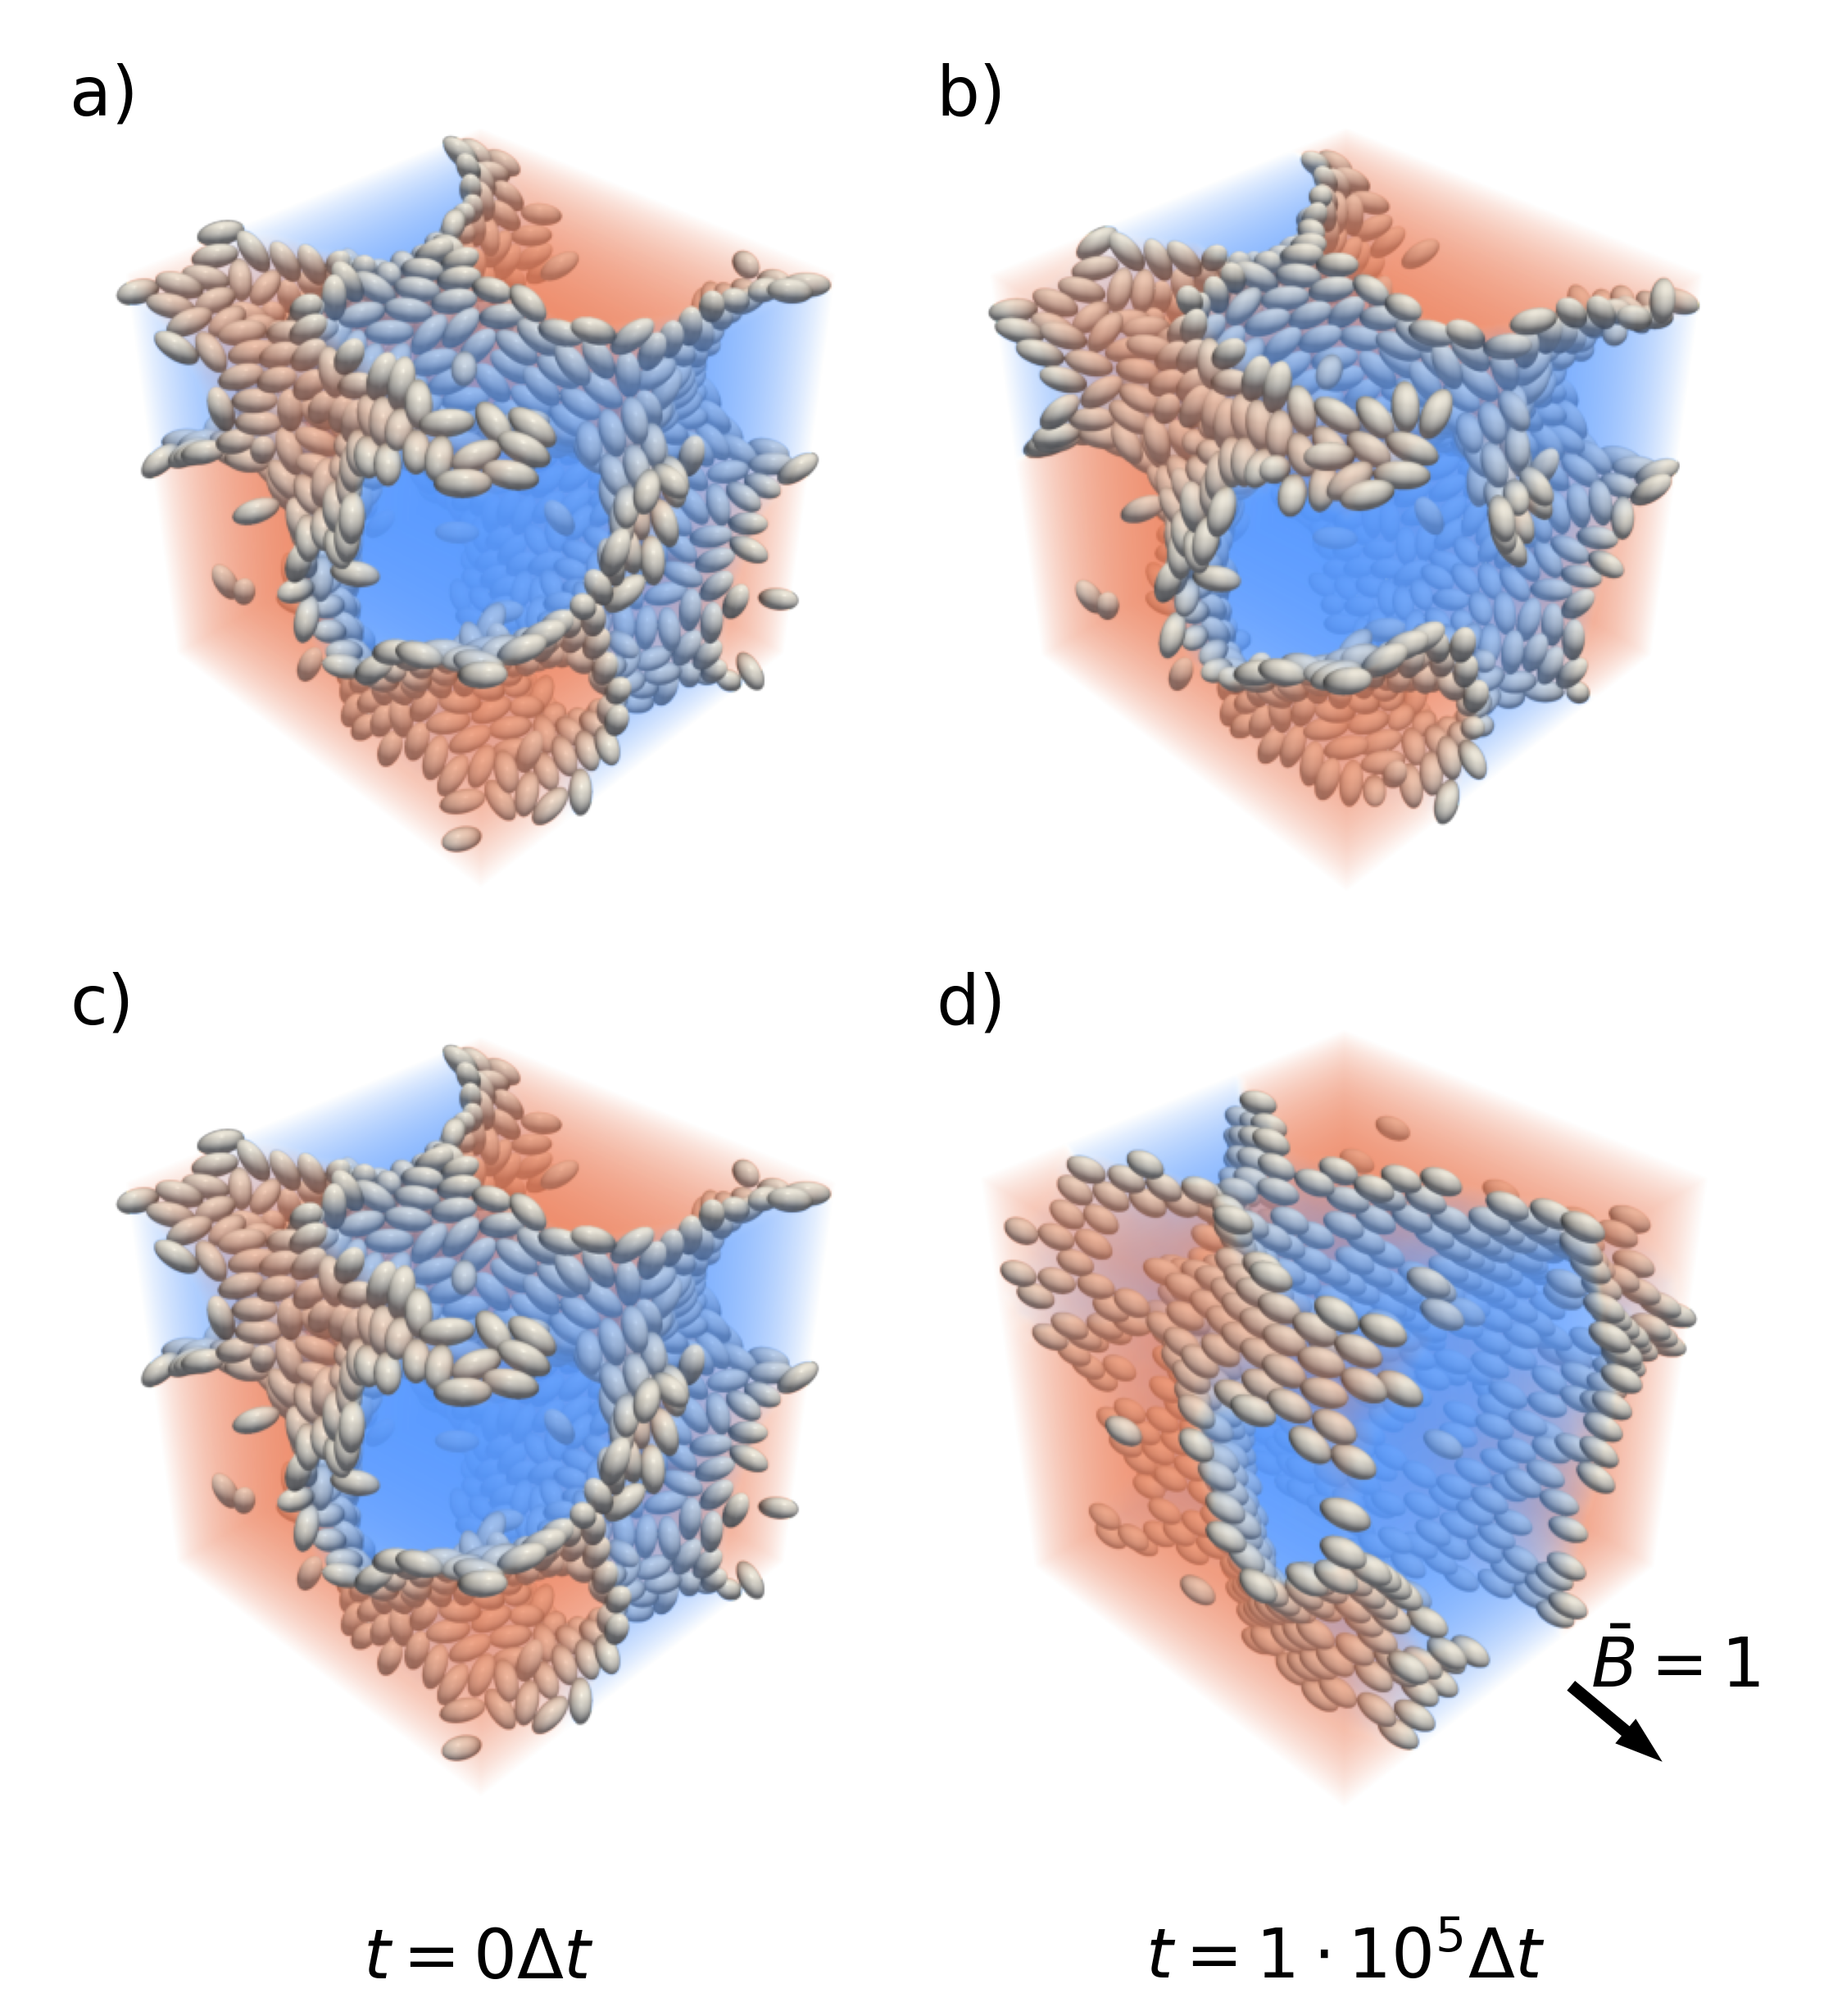
\includegraphics[scale=0.5]{../figures/results/paper2/microstructure_viz-field_on.png} 
\caption{Visualizations of bijels stabilized by prolate particles simulated under no fields at $t = 0$ (left columns) and $t = 10^5$ (right columns). The top 
         row detail the microstructure evolution for bijels with no applied field while the bottom rows show bijels stabilized by oblate and prolate particles 
         respectively with a field strength of $\bar{B} = 1$ applied.}
\label{fig:microstructure_viz-field_on} 
\end{figure}

Figure~\ref{fig:microstructure_viz-field_on} shows that at zero field, the fluid domains exhibit an isotropic, co-continuous morphology with particles randomly 
distributed and oriented at the fluid interface. Upon applying a magnetic field (\(\bar{B}_z = 1\)), the particles undergo reorientation along the field direction, 
which visibly alters the interfacial configuration and the domain morphology. 
To quantitatively characterize this response, we compute the average domain size as a function of time and magnetic field strength. Additionally, to assess 
how particle alignment contributes to the structural transition, we overlay the evolution of the nematic order parameter with the domain size. This correlation 
provides insight into the mechanistic role of particle ordering in driving microstructural transformation under applied magnetic fields \cite{veerman_phase_1992}.
The nematic order parameter is calculated from the orientations of the particles as    

\begin{equation}
\tens{Q} = \frac{1}{n_p} \sum_i \left( \frac{3}{2} \hat{\vec{o}}_i \otimes \hat{\vec{o}}_i -\frac{1}{2}\mathsf{1} \right) ,
\end{equation}

where \(\hat{\vec{o}}_i\) is the orientation of the \(i\)-th particles and \(n_p\) is the number of particles in the system. The largest eigenvalue of 
\(\tens{Q}\) yields the nematic order parameter

\begin{equation}
S = \left\langle \frac{3}{2}\cos^2 (\theta) - \frac{1}{2} \right\rangle ,
\end{equation}

where \(\theta=\arccos(\hat{\vec{o}}_i\cdot\hat{\vec{n}})\) is the angle between the particle orientation and the nematic director \(\hat{\vec{n}}\). We plot $S$
and $L$ over time in Figure \ref{fig:domain_size-field_on}

\begin{figure} 
\centering 
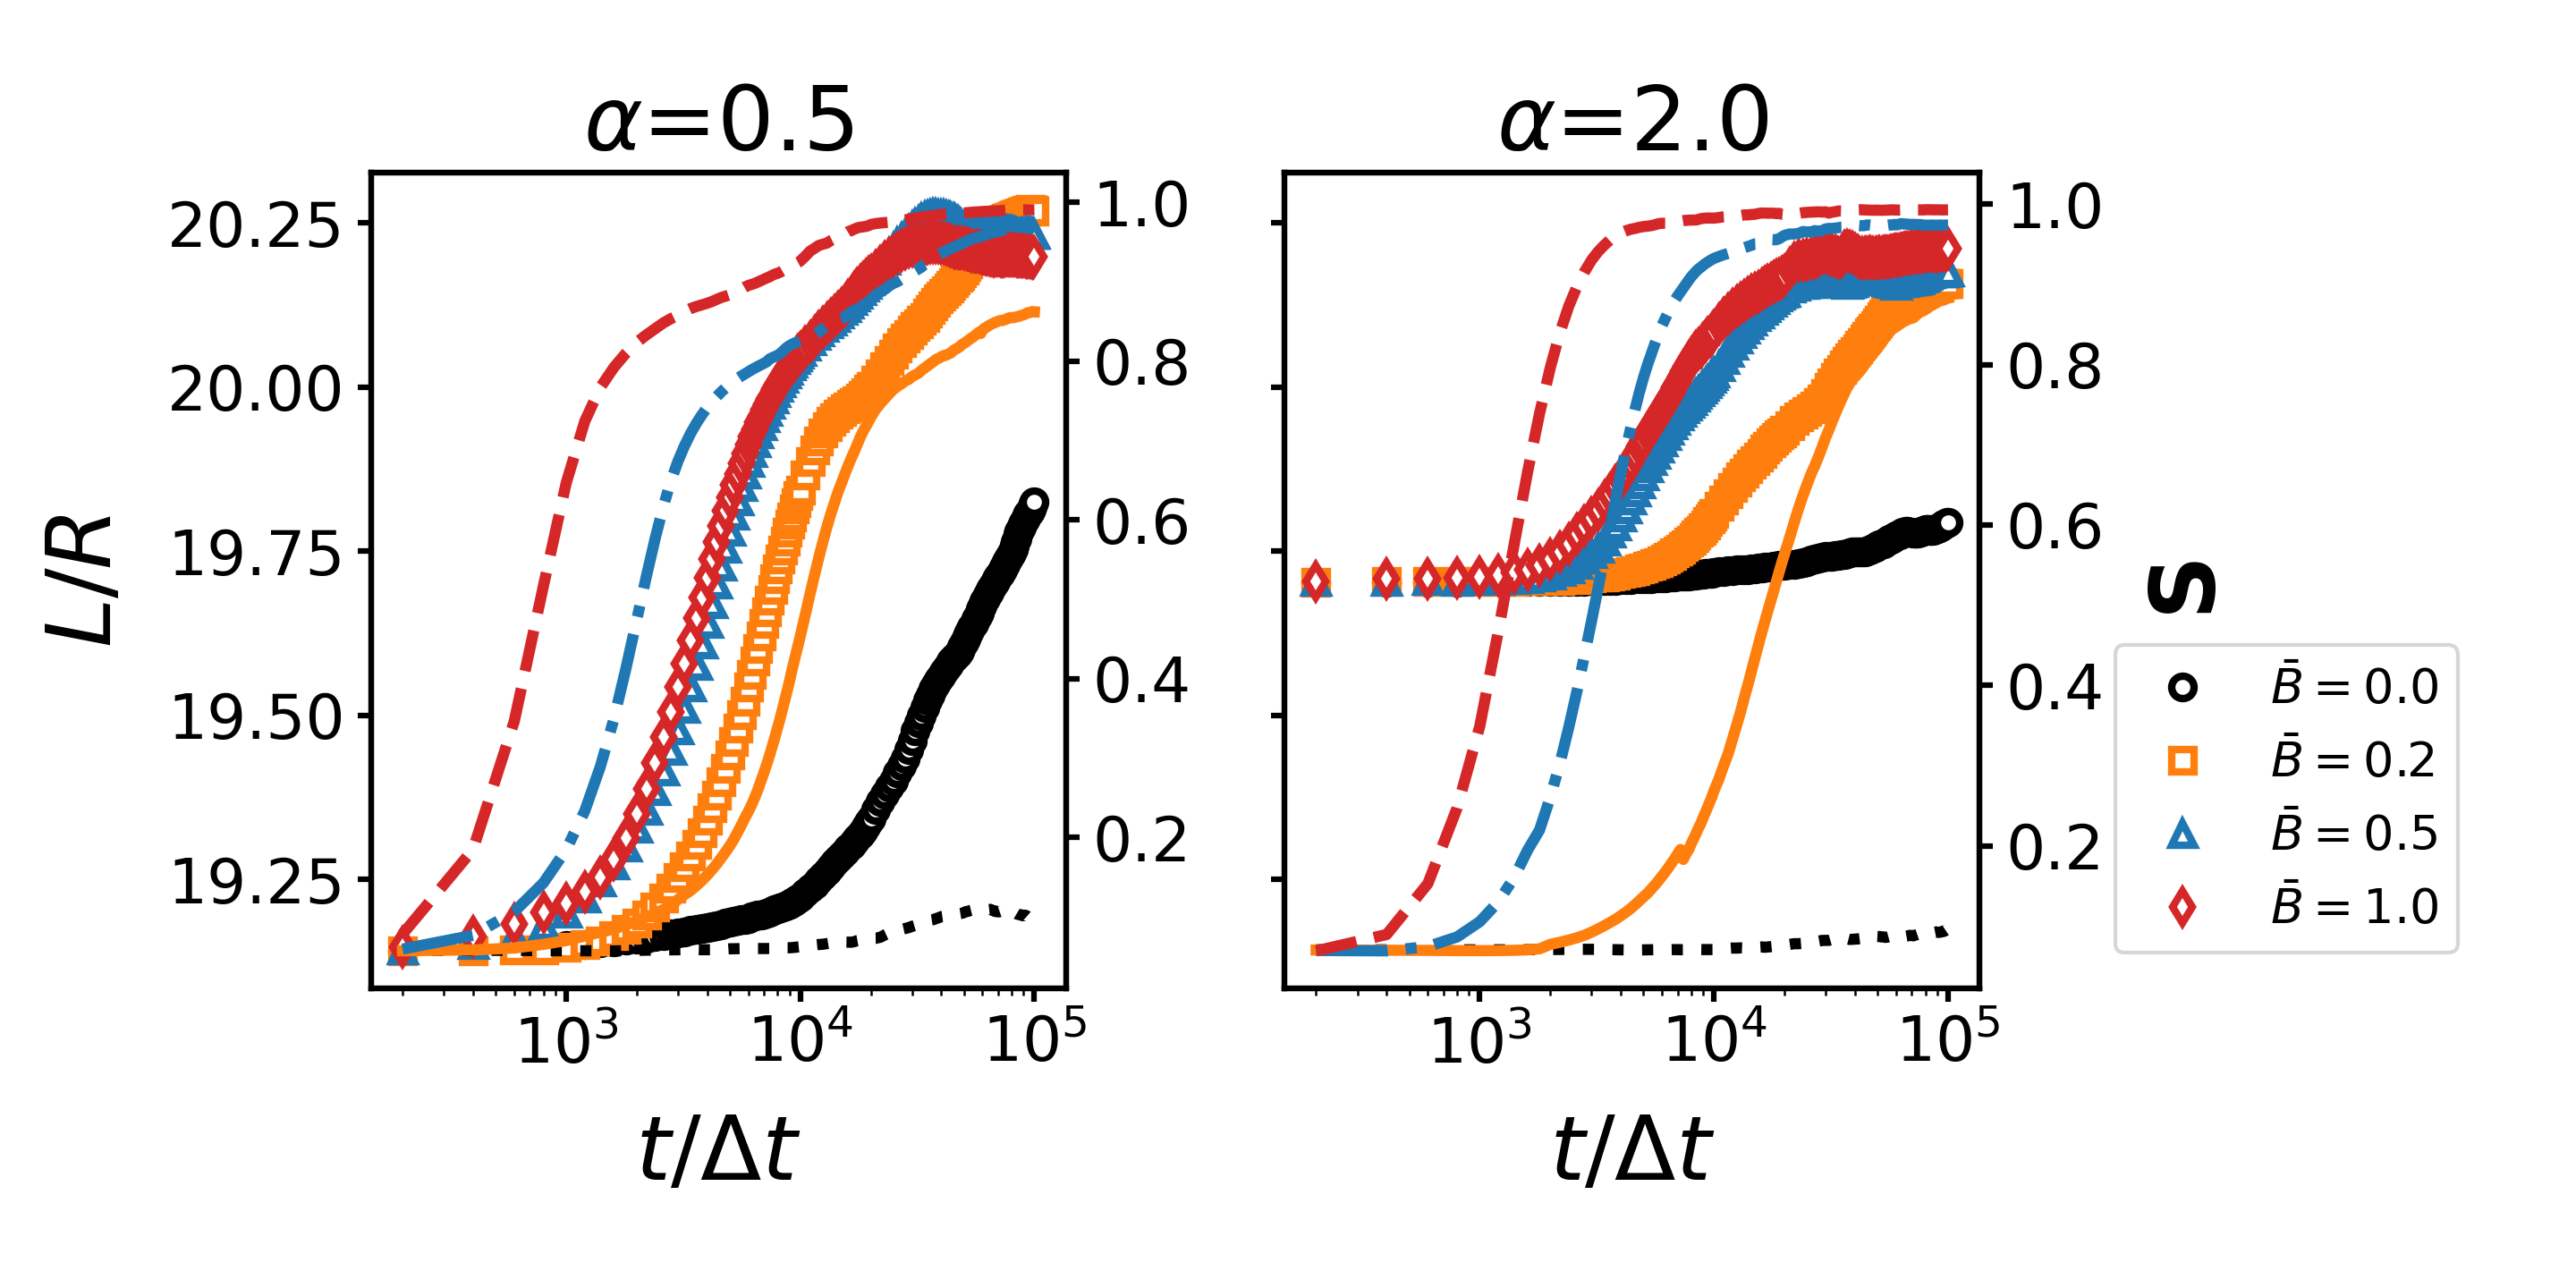
\includegraphics[scale=0.6]{../figures/results/paper2/domain_size-field_on.png} 
\caption{Plots of the time evolution of the normalized domain size \(L/R\) (markers) and nematic order parameter 
         \(S\) (lines) for bijels stabilized by oblate (left, \(\alpha = 0.5\)) and prolate (right, \(\alpha = 2.0\)) ellipsoidal particles under varying 
         magnetic field strengths. Here, \(R = 7.9\) is the volume-equivalent sphere radius.} 
\label{fig:domain_size-field_on} 
\end{figure}

The results show that applying a magnetic field to bijels 
initially formed without one induces domain coarsening, with the final domain size increasing by up to 5.2\% for oblate and 2.5\% for 
prolate particle-stabilized systems.
In both oblate and prolate systems, domain coarsening follows a characteristic three-stage evolution: an initial slow growth phase, a period of rapid 
coarsening, and eventual plateauing as the structure reaches a new jammed configuration. Even in the absence of a magnetic field (\(\bar{B}_z = 0\)), 
domain growth is observed driven by steric rearrangement of interfacial particles, consistent 
with findings by Günther et al.~\cite{gunther_timescales_2014}. Notably, the initiation of domain coarsening under applied magnetic fields is more rapid 
for bijels stabilized by oblate particles compared to prolate systems. However, the rejamming process takes longer.

In the absence of magnetic fields, a slight increase in $S(t)$ is observed, consistent with the sterically driven reorientation of particles at the interface.
\cite{gunther_timescales_2014} Upon application of a magnetic field, the curves for \(S(t)\) increase before plateauing, indicating the parameter has reached
its saturation value. Notably at stronger field strengths, $S(t)$ precedes the increase in domain size for both particle shapes analyzed. This time lag suggests 
that nematic ordering is a precursor, but not the sole driver, of domain coarsening. Overall, these results confirm that domain coarsening in magnetically 
responsive bijels occurs as a result of applied magnetic fields, with the degree of change observed dependent on the strength of the applied field. 

\subsubsection{Particle reorientation at the interface}

Building on the observed time lag between the onset of particle alignment and domain coarsening, we next investigate the underlying dynamics of particles at the 
interface. While nematic ordering appears to precede structural changes, the delayed increase in domain size at higher magnetic field strengths suggests that 
additional factors influence the system's response. In this context, capillary interactions between particles and the fluid interface, as well as steric hindrance 
from neighboring particles, may act to resist or slow particle rearrangement, thereby affecting the timescale of domain evolution. To better understand these 
phenomena, we focus on the dynamic behavior of the interfacial particle monolayer. As a first step, we visualize the initial and final configurations of bijels 
stabilized by prolate ellipsoids before and after application of a magnetic field, providing qualitative insight into particle displacement and reorganization 
at the interface.

\begin{figure} 
\centering 
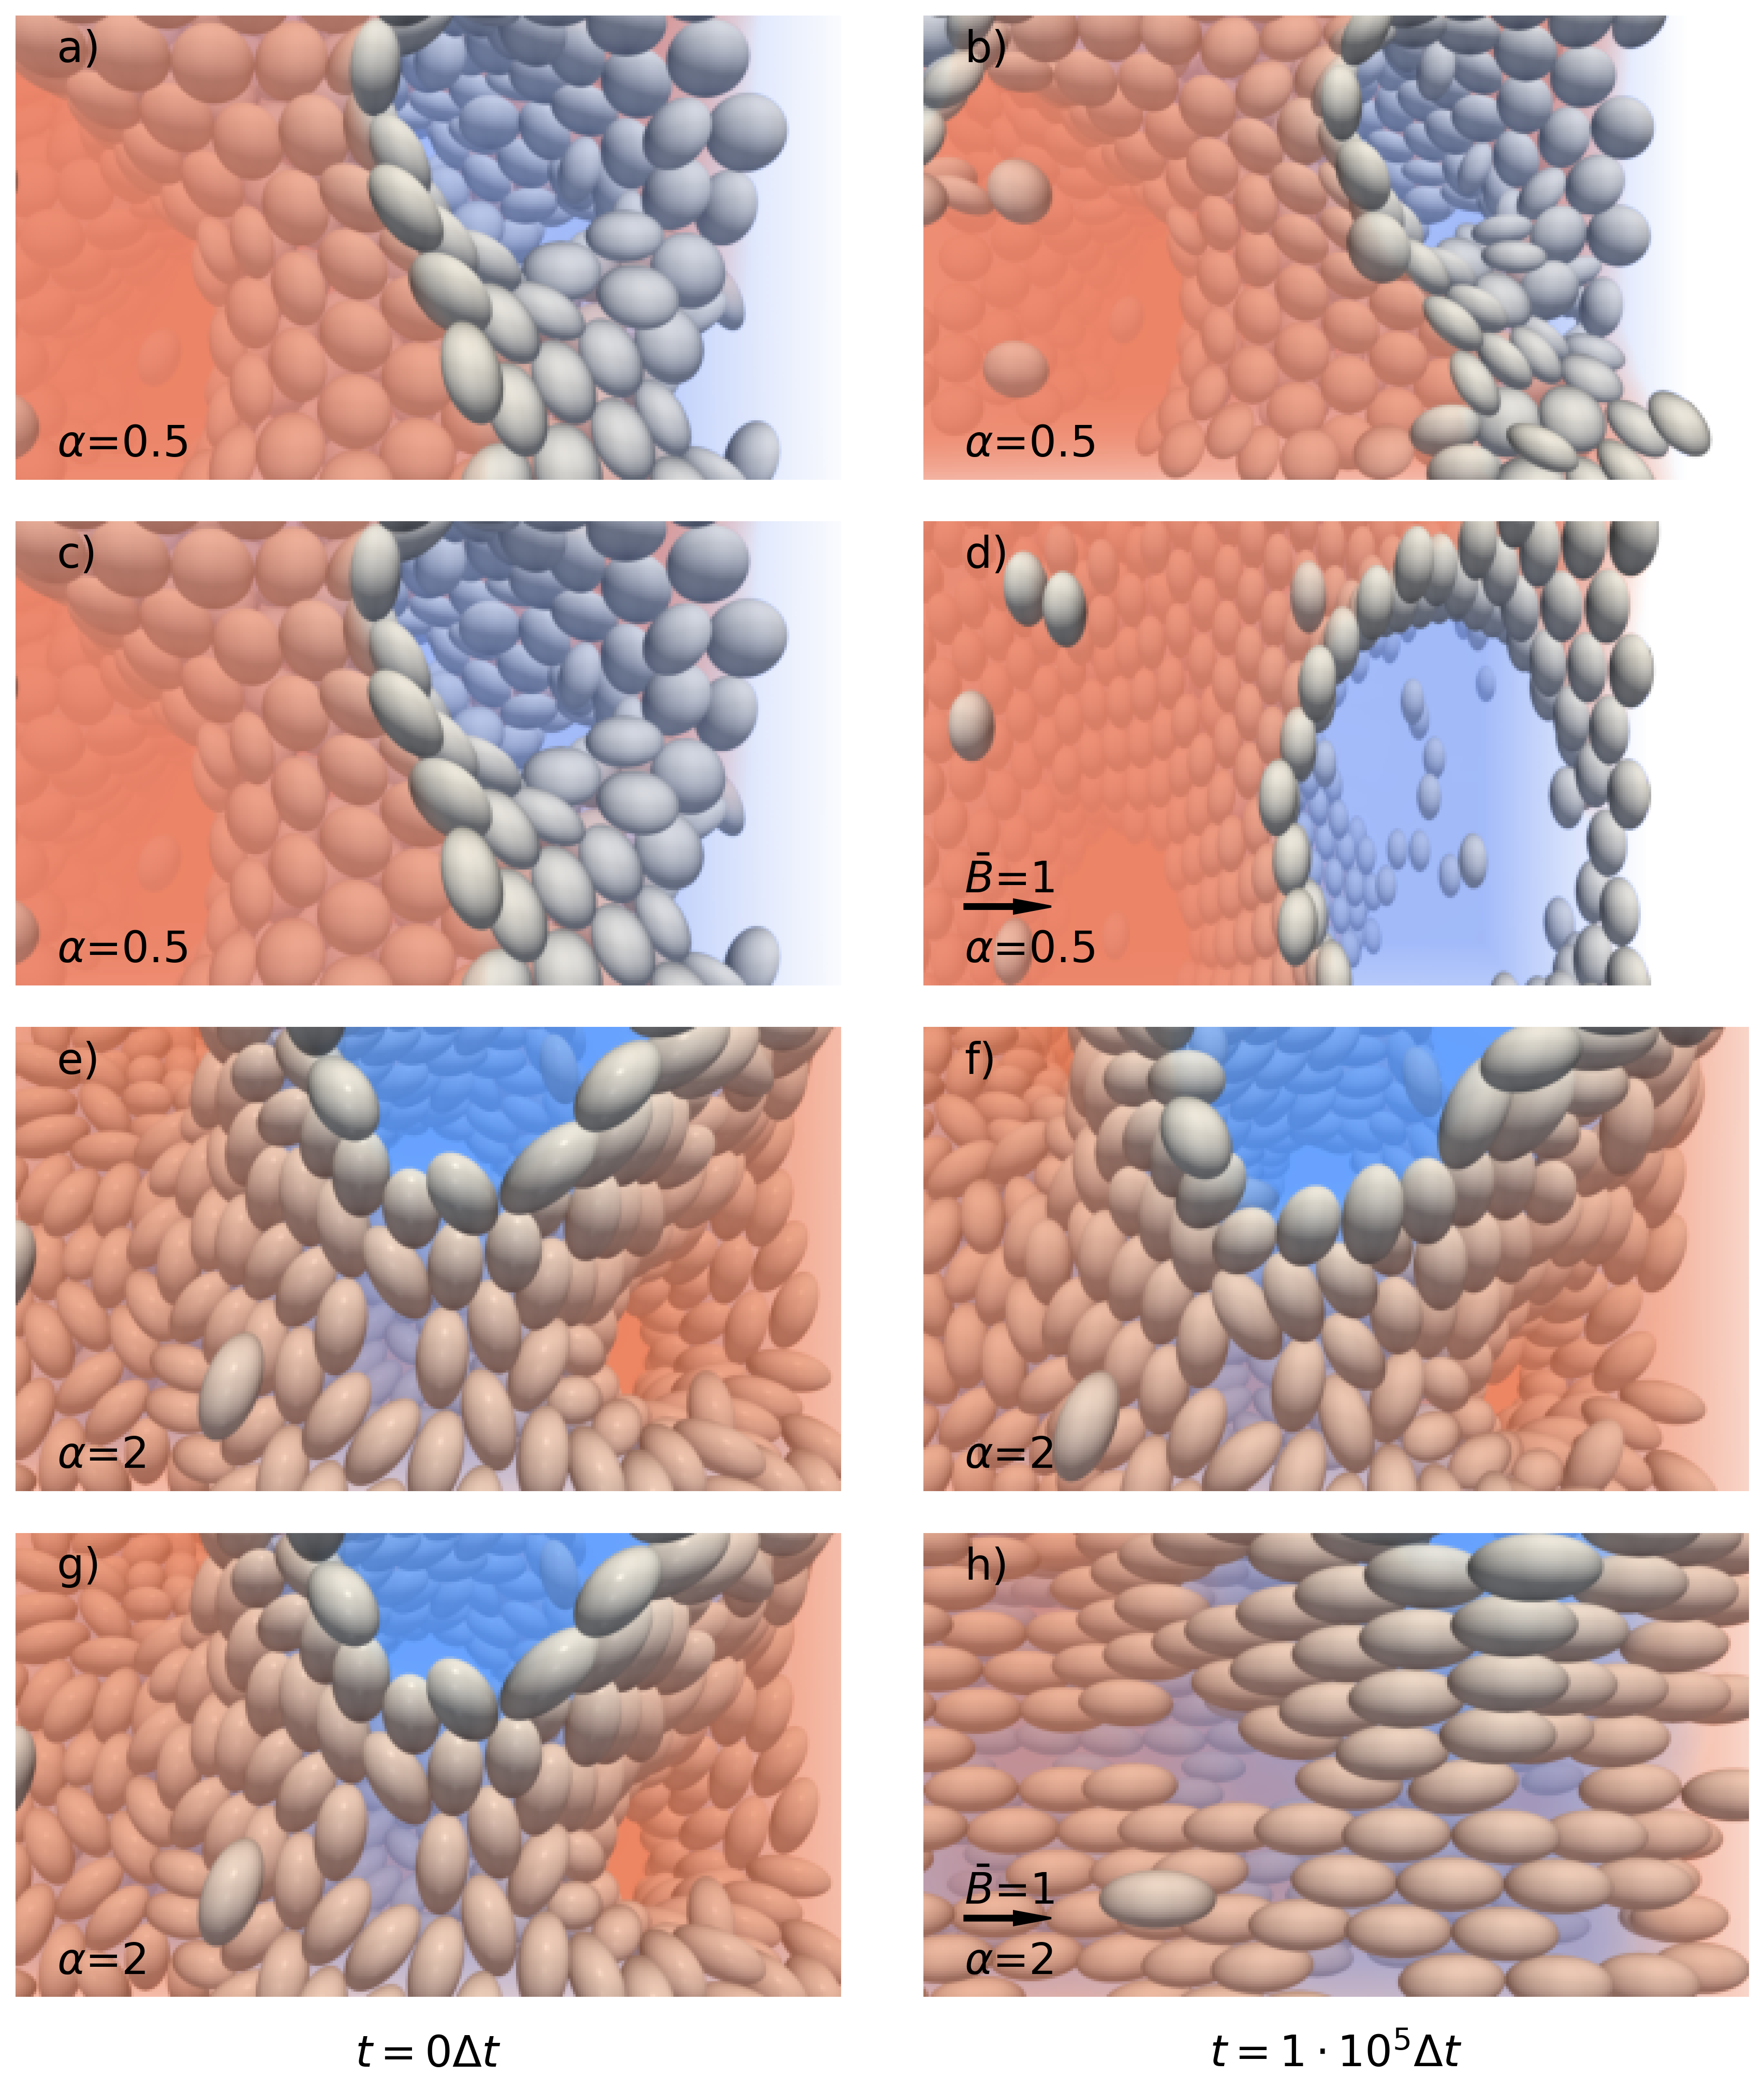
\includegraphics[scale=0.4]{../figures/results/paper2/particle_viz-field_on.png} 
\caption{Visualizations of bijels stabilized by prolate ellipsoidal particles at the initial and final timesteps, 
         both in the absence of a magnetic field (top row) and with a magnetic field applied (\(\bar{B}_z = 1\), bottom row). Particle reorientation to the
         applied field can be observed.} 
\label{fig:particle_viz-field_on} 
\end{figure}

The snapshow shows that in the absence of a magnetic field, minor variations in particle orientation and position occur due to steric interactions, as 
previously observed by Günther et al.~\cite{gunther_timescales_2014}. However, the application of a magnetic field induces clear orientational ordering of the 
particle monolayer, with particles aligning along the field direction and reorganizing into distinct interfacial arrangements. These changes suggest that both 
capillary forces and steric hindrance are modified upon field application. While particles naturally prefer to lie flat at the interface to minimize interfacial 
adsorption energy, the applied field competes with this tendency, reorienting the particles and disrupting their initial packing.

To quantify the orientation of the particles relative to the interface, we analyzed the angle between each particles symmetry axis and 
the local interface normal. We generated a mesh of the interface using the marching cubes algorithm and, for each particle, identified the nearest mesh vertex 
(excluding those beyond the length of the particle's long axis). We then calculated the angle \(\psi\) between the particle orientation vector 
\(\hat{\vec{o}}_i\) and the local surface normal. We plot the time evolution of $\psi$ in Figure \ref{fig:interface_angle-field_on}.

\begin{figure} 
    \centering 
    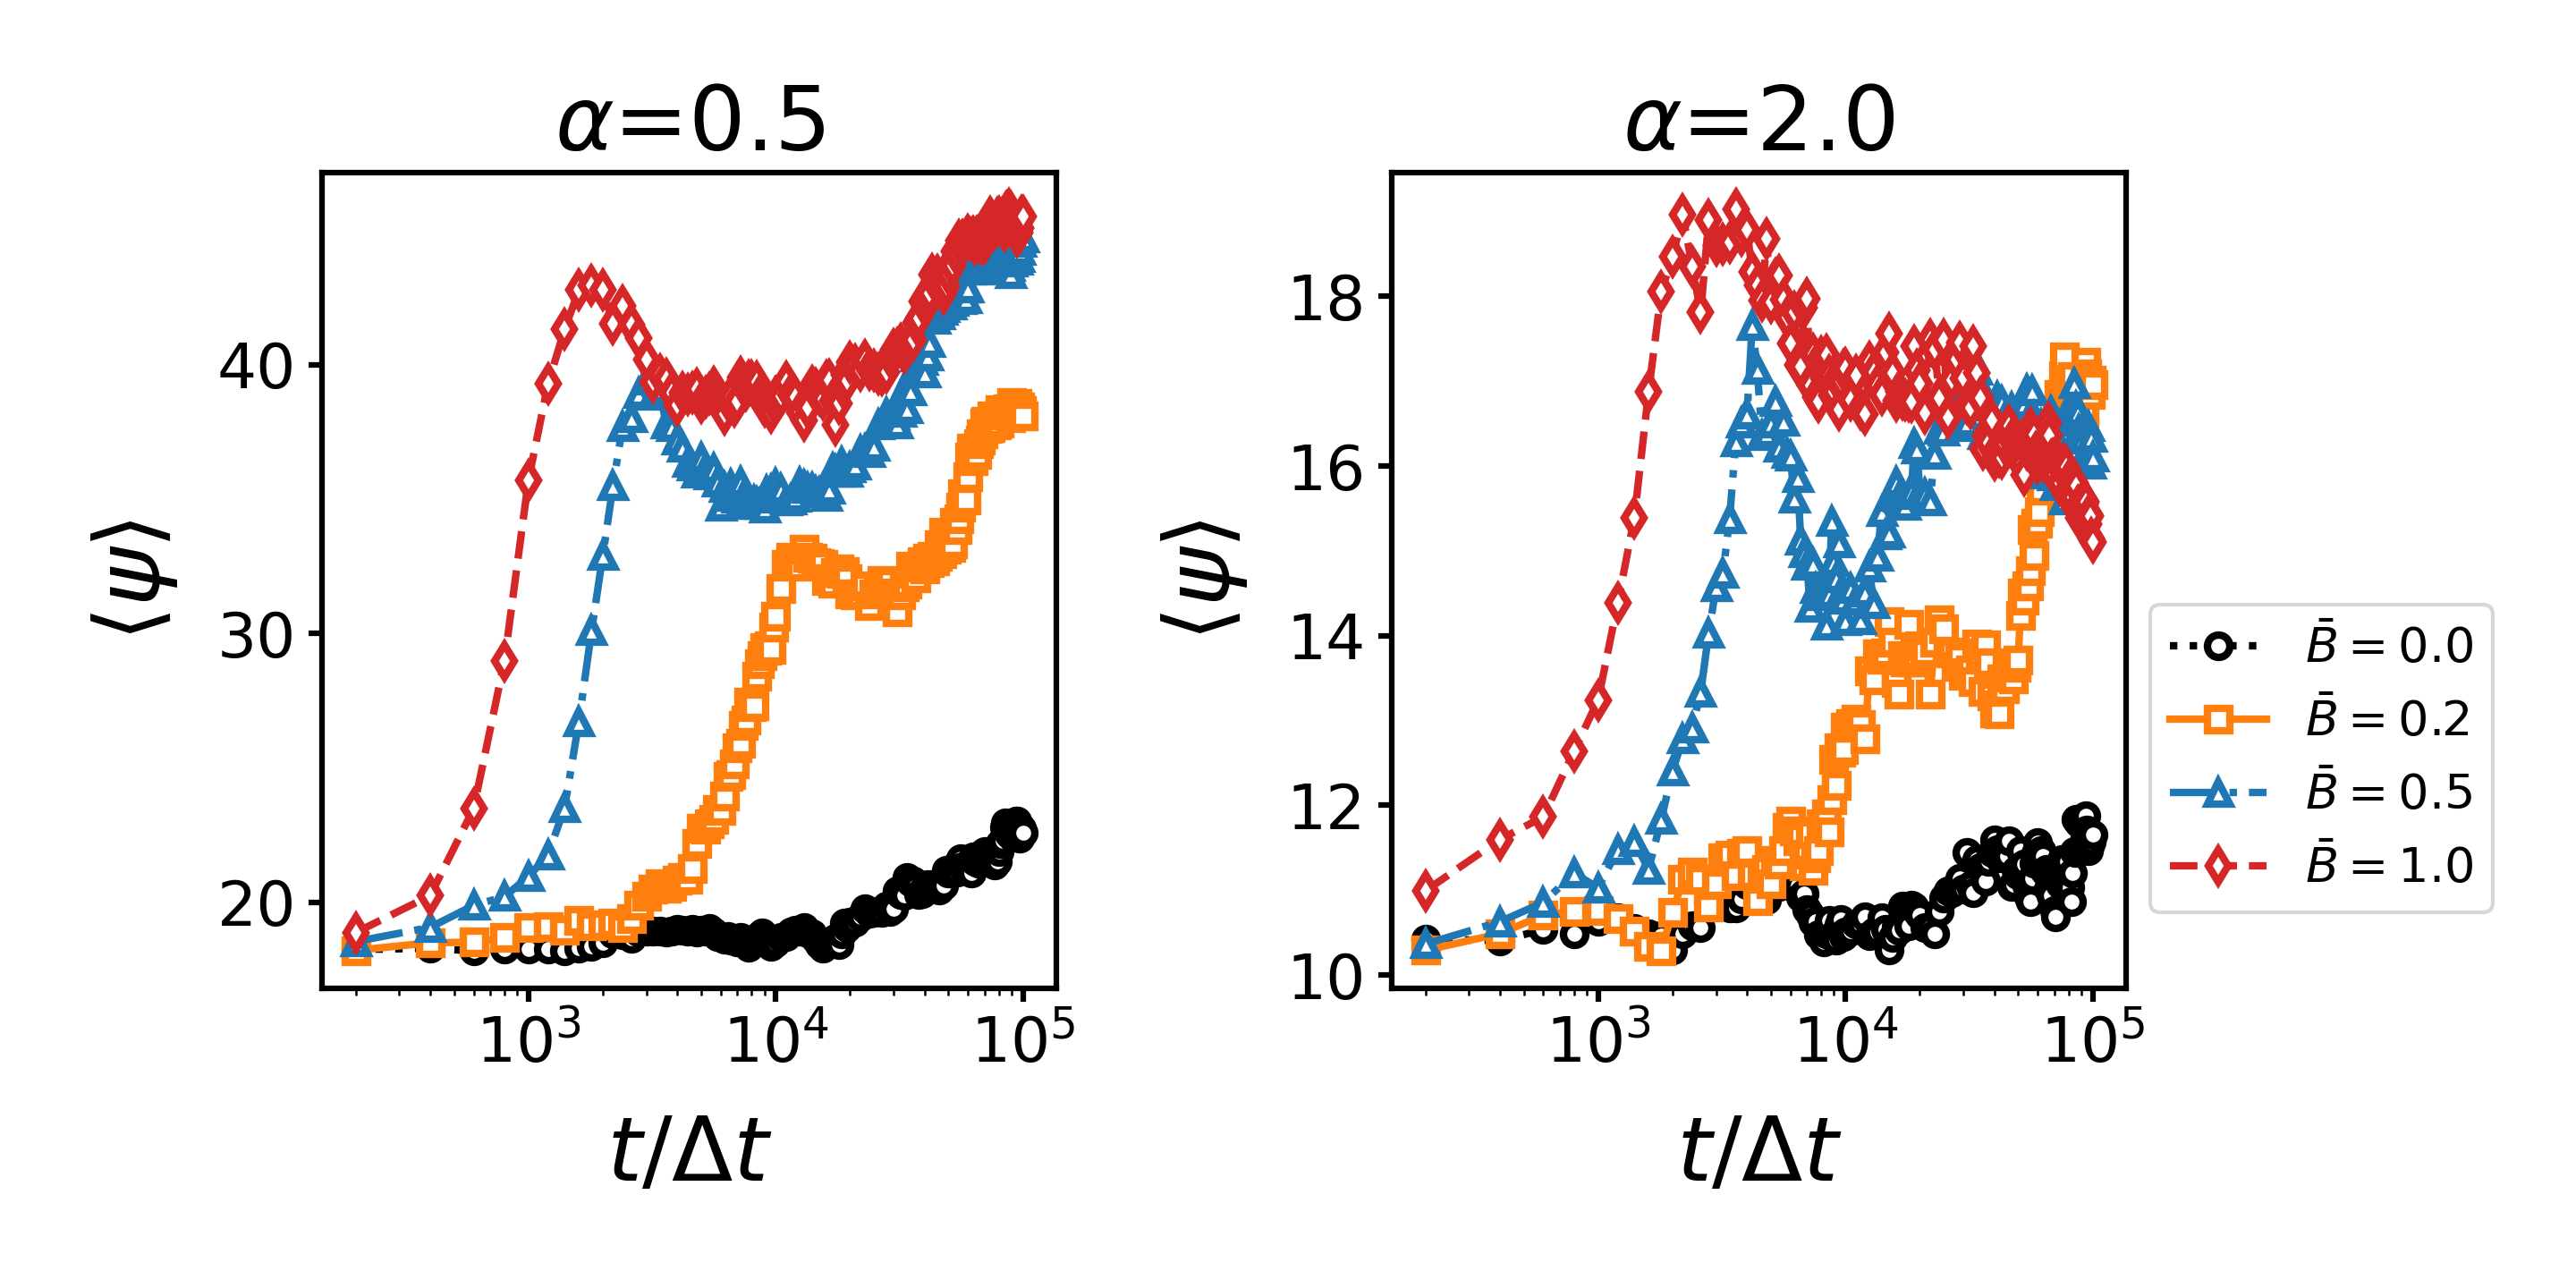
\includegraphics[scale=0.6]{../figures/results/paper2/psi-field_on.png} 
    \caption{Plots of the evolution of the average interface angle \(\langle \psi \rangle\) over time for bijels stabilized 
             by oblate (left) and prolate (right) ellipsoidal particles under varying magnetic field strengths. The response of \(\langle \psi \rangle\) 
             differs notably between the two particle morphologies.} 
    \label{fig:interface_angle-field_on} 
\end{figure}

For bijels stabilized by oblate particles, \(\langle \psi \rangle\) initially increases from approximately \(19^\circ\), indicating that the particles, which begin 
in an approximately flat configuration at the interface, begin to tilt out of the plane in response to the applied field. After a brief decrease or plateau, the angle 
resumes increasing before stabilizing. This behavior suggests that particles first reorient under magnetic torque but are temporarily resisted by interfacial tension 
and capillary constraints. Once the interface begins to deform in response to particle tilt, the system eventually jams in a new configuration, locking the particles 
at an elevated angle. Both the rate of initial tilt and the duration of the plateau phase increase with field strength, and the final value of 
\(\langle \psi \rangle\) is positively correlated with the magnitude of the applied field.

For bijels stabilized by prolate particles, a similar but more subtle trend is observed. The initial value of \(\langle \psi \rangle\) starts around \(10^\circ\), 
gradually increases, and then exhibits a small plateau followed by a slight decline. While the rate and magnitude of the initial increase are field-dependent, 
the final values converge more closely across different field strengths, suggesting that the field sensitivity of interface tilt is weaker for prolate particles. 
The overall changes in \(\langle \psi \rangle\) are also smaller in magnitude compared to those in oblate systems, indicating that prolate particles experience 
less pronounced reorientation at the interface.

While the interface angle \(\langle \psi \rangle\) provides insight into the out-of-plane orientation of particles in response to magnetic field application, 
it does not capture how particles reorganize at the interface, observed in Figure \ref{fig:microstructure_viz-field_on} Since the evolution of microstructure is 
influenced not only by tilt but also by the steric effects of interfacial particles, we also assess the Steinhardt bond orientational parameter. 
We compute the six fold bond orienational parameter $q_6$ which measures the degree of hexagonal arrangement of particles at the interface.
\cite{steinhardt_bond-orientational_1983, lechner_accurate_2008, mickel_shortcomings_2013} These parameters characterize the local structural ordering by projecting 
the orientations of neighboring particles onto spherical harmonics of degree \(l\), and are defined as

\begin{equation}
q_l(i) = \left( \frac{4\pi}{2l+1} \sum_{m=-l}^{l} \left| \frac{1}{N(i)} \sum_{j=1}^{n(i)} Y_{lm}(\vec{r}_{ij}) \right|^2 \right)^{\frac{1}{2}} ,
\end{equation} 
%\TODO{update formula to the one actually used}

Here, \(n(i)\) denotes the number of nearest neighbors of particle \(i\), \(\vec{r}_{ij}\) is the vector connecting the centers of particles \(i\) and \(j\), and 
\(m\) is an integer ranging from \(-l\) to \(l\) that indexes the spherical harmonic components \(Y_{lm}\). Neighbor lists are typically defined using a fixed cutoff 
radius around each particle, identifying nearby particles as neighbors. We calculate the python package Freud to calculate the bond order parameters and use a Voronoi 
cell to determine the particle neighborhood rather than the standard distance criterion \cite{ramasubramani_freud_2020,mickel_shortcomings_2013}. The Voronoi-based 
method avoids the need for a predefined cutoff and yields more robust neighbor definitions, particularly in disordered systems. Bond orientational order parameters 
have been widely employed to study structural transitions in colloidal and ceramic systems, including crystallization, nucleation, and glass formation 
\cite{vagberg_glassiness_2011, besseling_three-dimensional_2007, schall_structural_2007, ozawa_jamming_2012} We plot the time evolution of $\psi$ in Figure 
\ref{fig:Q6-field_on}.

\begin{figure} 
    \centering 
    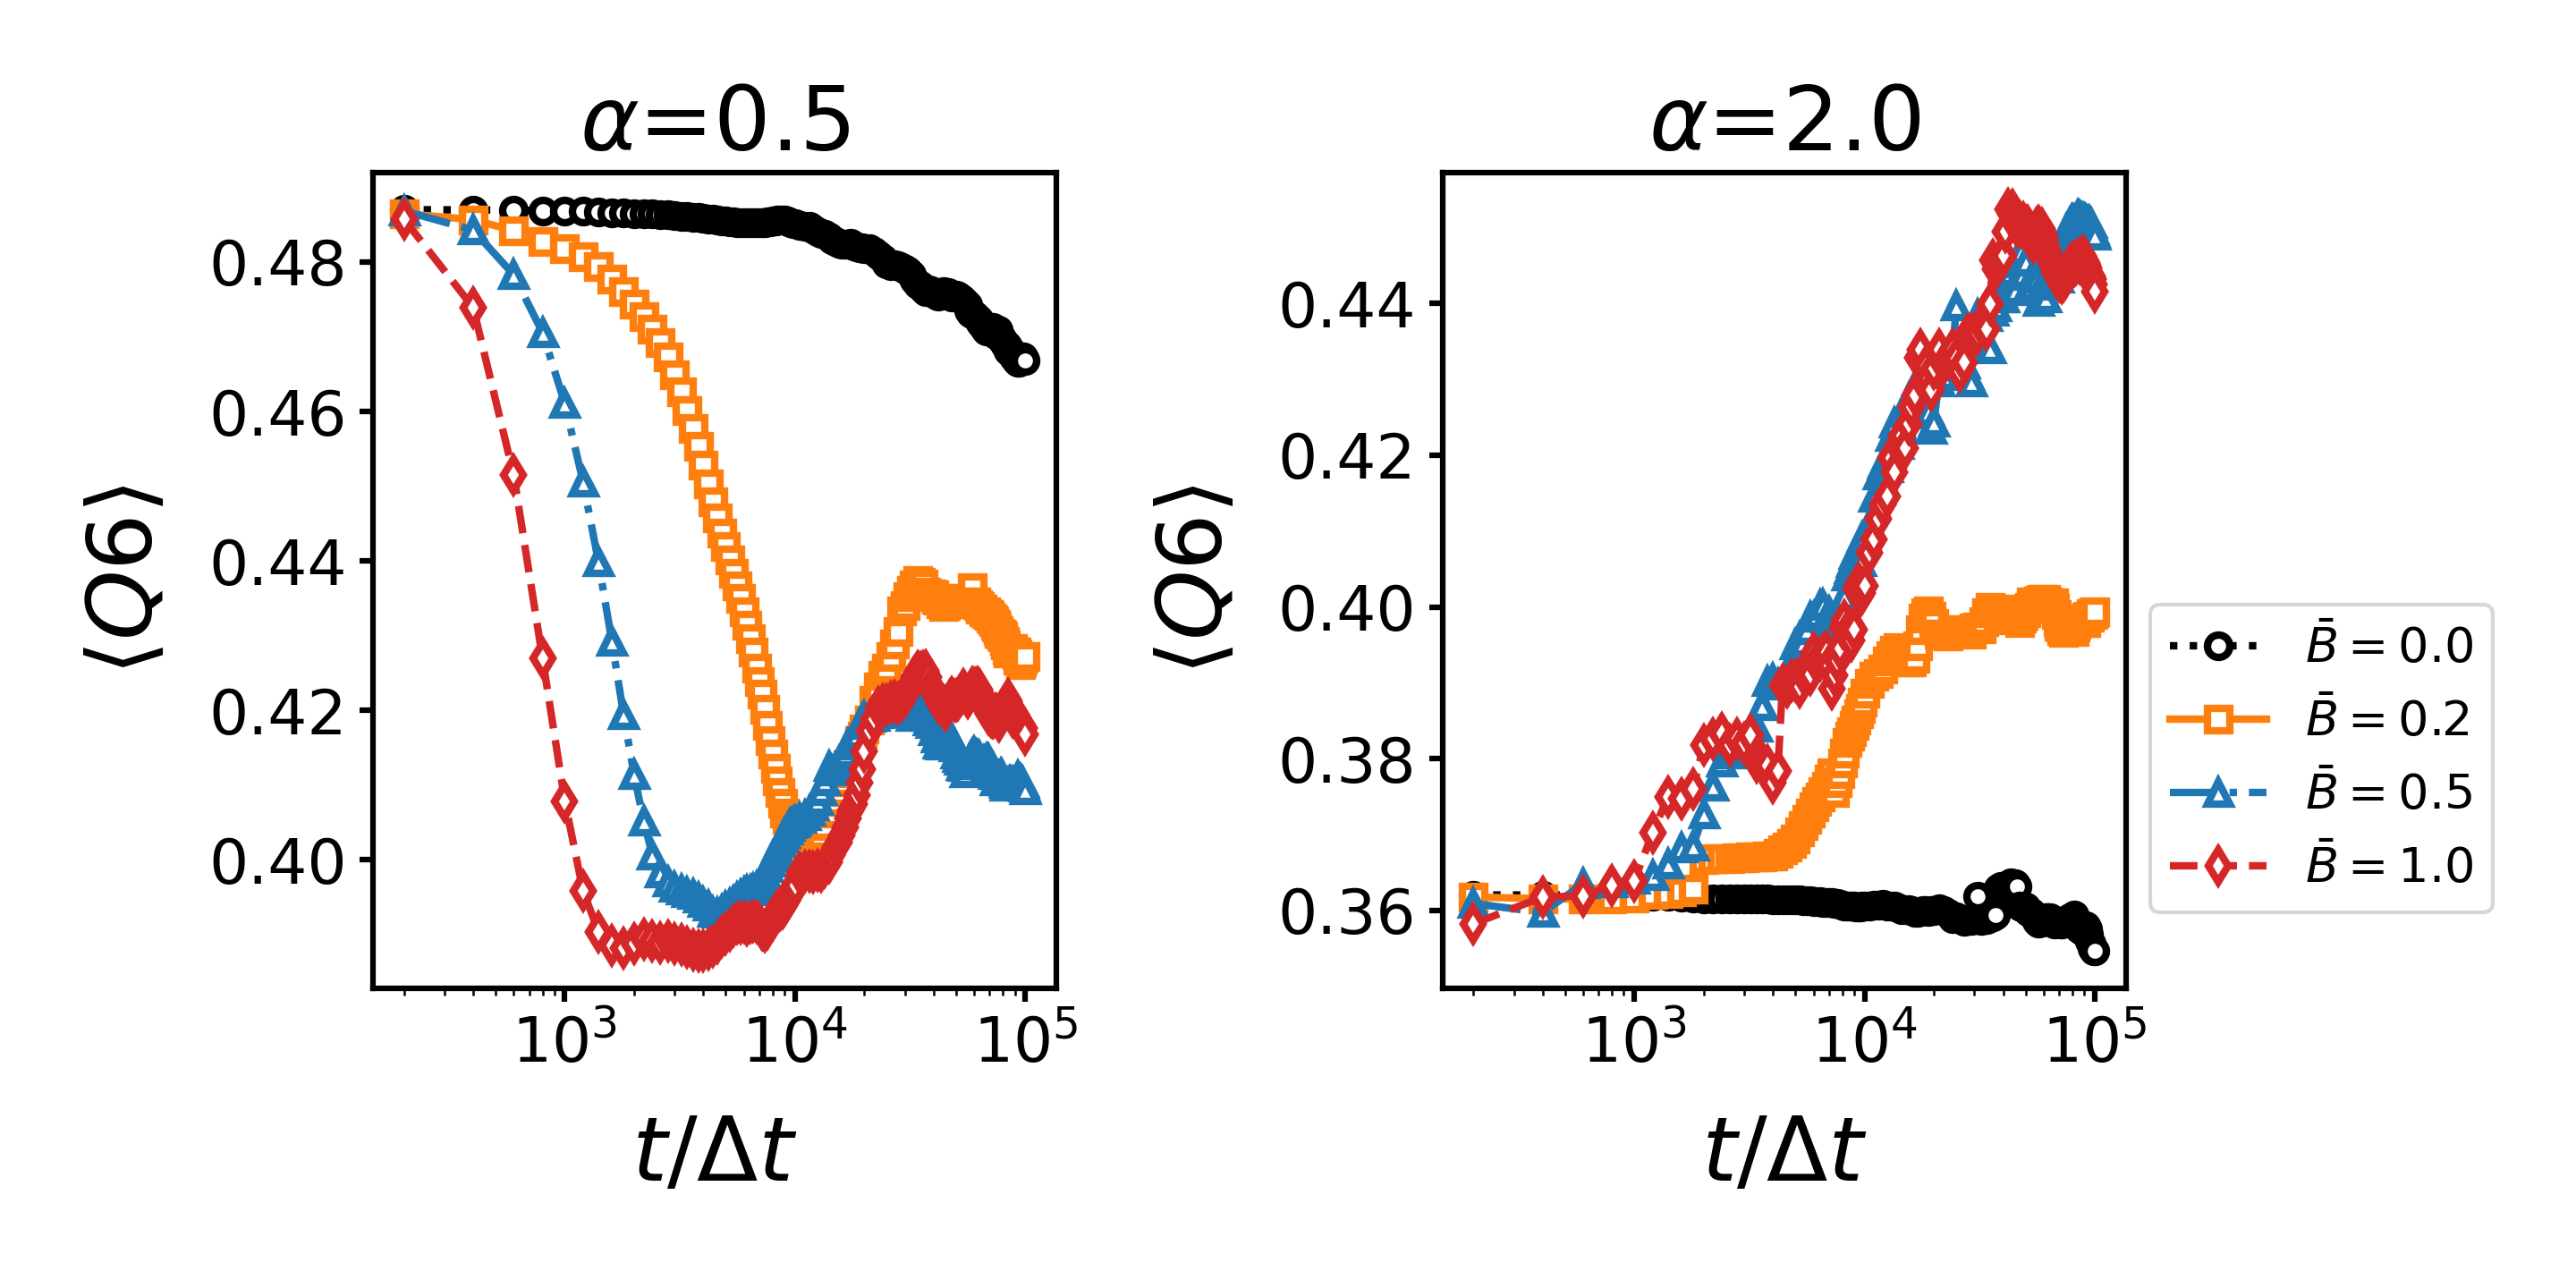
\includegraphics[scale=0.6]{../figures/results/paper2/Q6-field_on.png} 
    \caption{Plots of the time evolution of the six-fold Steinhardt bond order parameter \(\langle Q_6 \rangle\) for bijels 
             stabilized by oblate (left) and prolate (right) ellipsoidal particles under varying magnetic field strengths. The dynamics of interfacial ordering differ 
             significantly between particle morphologies with \(\langle Q_6 \rangle\) decreasing over time for oblate particles and increasing for prolate particles.} 
    \label{fig:Q6-field_on} 
\end{figure}

From Figure \ref{fig:Q6-field_on} the time evolution of \(\langle Q_6 \rangle\) can be qualitatively divided into three regimes;
an initial transition period, a plateau, and a final reordering or jamming phase.
For oblate particles, application of the magnetic field initially causes a sharp decrease in \(\langle Q_6 \rangle\), reflecting a disruption of the 
pre-existing interfacial order as particles begin to tilt and rearrange. This is followed by a plateau, during which ordering is temporarily suppressed 
as particles continue reorienting. Finally, \(\langle Q_6 \rangle\) begins to increase gradually, indicating partial recovery of local order as the system 
evolves toward a new jammed state. The rate of change of \(\langle Q_6 \rangle\) significantly decreases toward the end of the simulation, suggesting the onset 
of kinetic arrest. The final value of \(\langle Q_6 \rangle\) is dependent on the applied magnetic field strength, with higher field strengths 
resulting in lower final ordering, potentially due to increased variance in the interfacial angle, reducing packing efficiency.

In contrast, for bijels stabilized by prolate particles, \(\langle Q_6 \rangle\) increases monotonically with time after the field is applied. The degree 
of ordering and the rate of increase both scale positively with magnetic field strength. The early stage is characterized by a modest rise in \(\langle Q_6 \rangle\), 
followed by a more rapid growth and eventual plateau, indicating progressive in-plane reordering of the particle monolayer as alignment along the field direction 
becomes dominant. The timing and extent of these regimes are also field-dependent with stronger fields result in earlier onset of ordering and higher final values 
of \(\langle Q_6 \rangle\). Notably, for all applied fields, the final ordering significantly exceeds that of the zero-field case. These results highlight that the 
response of interfacial particle order to magnetic fields is morphology-specific as oblate particles undergo a disruption and partial recovery of order, 
while prolate particles experience continuous enhancement of local ordering. 

\subsubsection{Microstructural effects of particle reordering}

Karthikeyan and Schiller identified that the reorientation of particles at the interface due to the application of magnetic fields caused domain size anisotropy
driven by the directional cessation of domain coarsening. \cite{karthikeyan_formation_2024} In this study, we have established that the mechanism of domain size change
arises from magnetic field driven rotations of particles at the interface, causing unjamming of the particle monolayer before rejamming and locking in the new
microstructure. Due to the differences in mechanism, we turn to investigate the anisotropic microstructure of the bijel at the final timestep. 

We probe the domain anisotropy using the directional second moment of the structure factor, computed along each Cartesian axis from the full structure factor shown
below. \cite{jansen_bijels_2011, gunther_timescales_2014}. 
    %
    \begin{equation}
    L_\beta(t)=2\pi\sqrt{\frac{\sum_{\vec{k}}S(\vec{k},t)}{\sum_{\vec{k}}k_\beta^2 S(\vec{k},t)}} .
    \end{equation}
    %
    This allows us to compute a domain size parallel
    (\(L_\parallel=L_z\)) and perpendicular (\(L_\perp=(L_x+L_y)/2\)) to the
    direction of \(\vec{B}\) separately. The average domain size \(L_d(t)\)
    is computed as \(L_d(t)=\sum_\beta L_\beta(t) / 3\).
    %
    \begin{equation}
    L_d(t)=2\pi\sqrt{\frac{\sum_{\vec{k}}S(\vec{k},t)}{\sum_{\vec{k}}\sum_\beta k_\beta^2 S(\vec{k},t)}} .
    \end{equation}
    %
Previous studies have also shown that a domain size increase is usually accompanied by a decrease in
tortuosity. \cite{karthikeyan_formation_2024} To determine whether these structural 
changes impact macroscopic transport properties, we also analyzed the tortuosity of the bijels. We utilize the package \texttt{taufactor} that implements
a periodic boundary condition solver and calculates the diffusive tortuosity of the bijel structures. Porous structures were 
extracted by binarizing the final order parameter field using a zero threshold, isolating the largest connected (percolating) domain. We plot the results of
the directional domain size and tortuosity in Figure \ref{fig:domain_size_aniso-field_on}

\begin{figure} 
    \centering 
    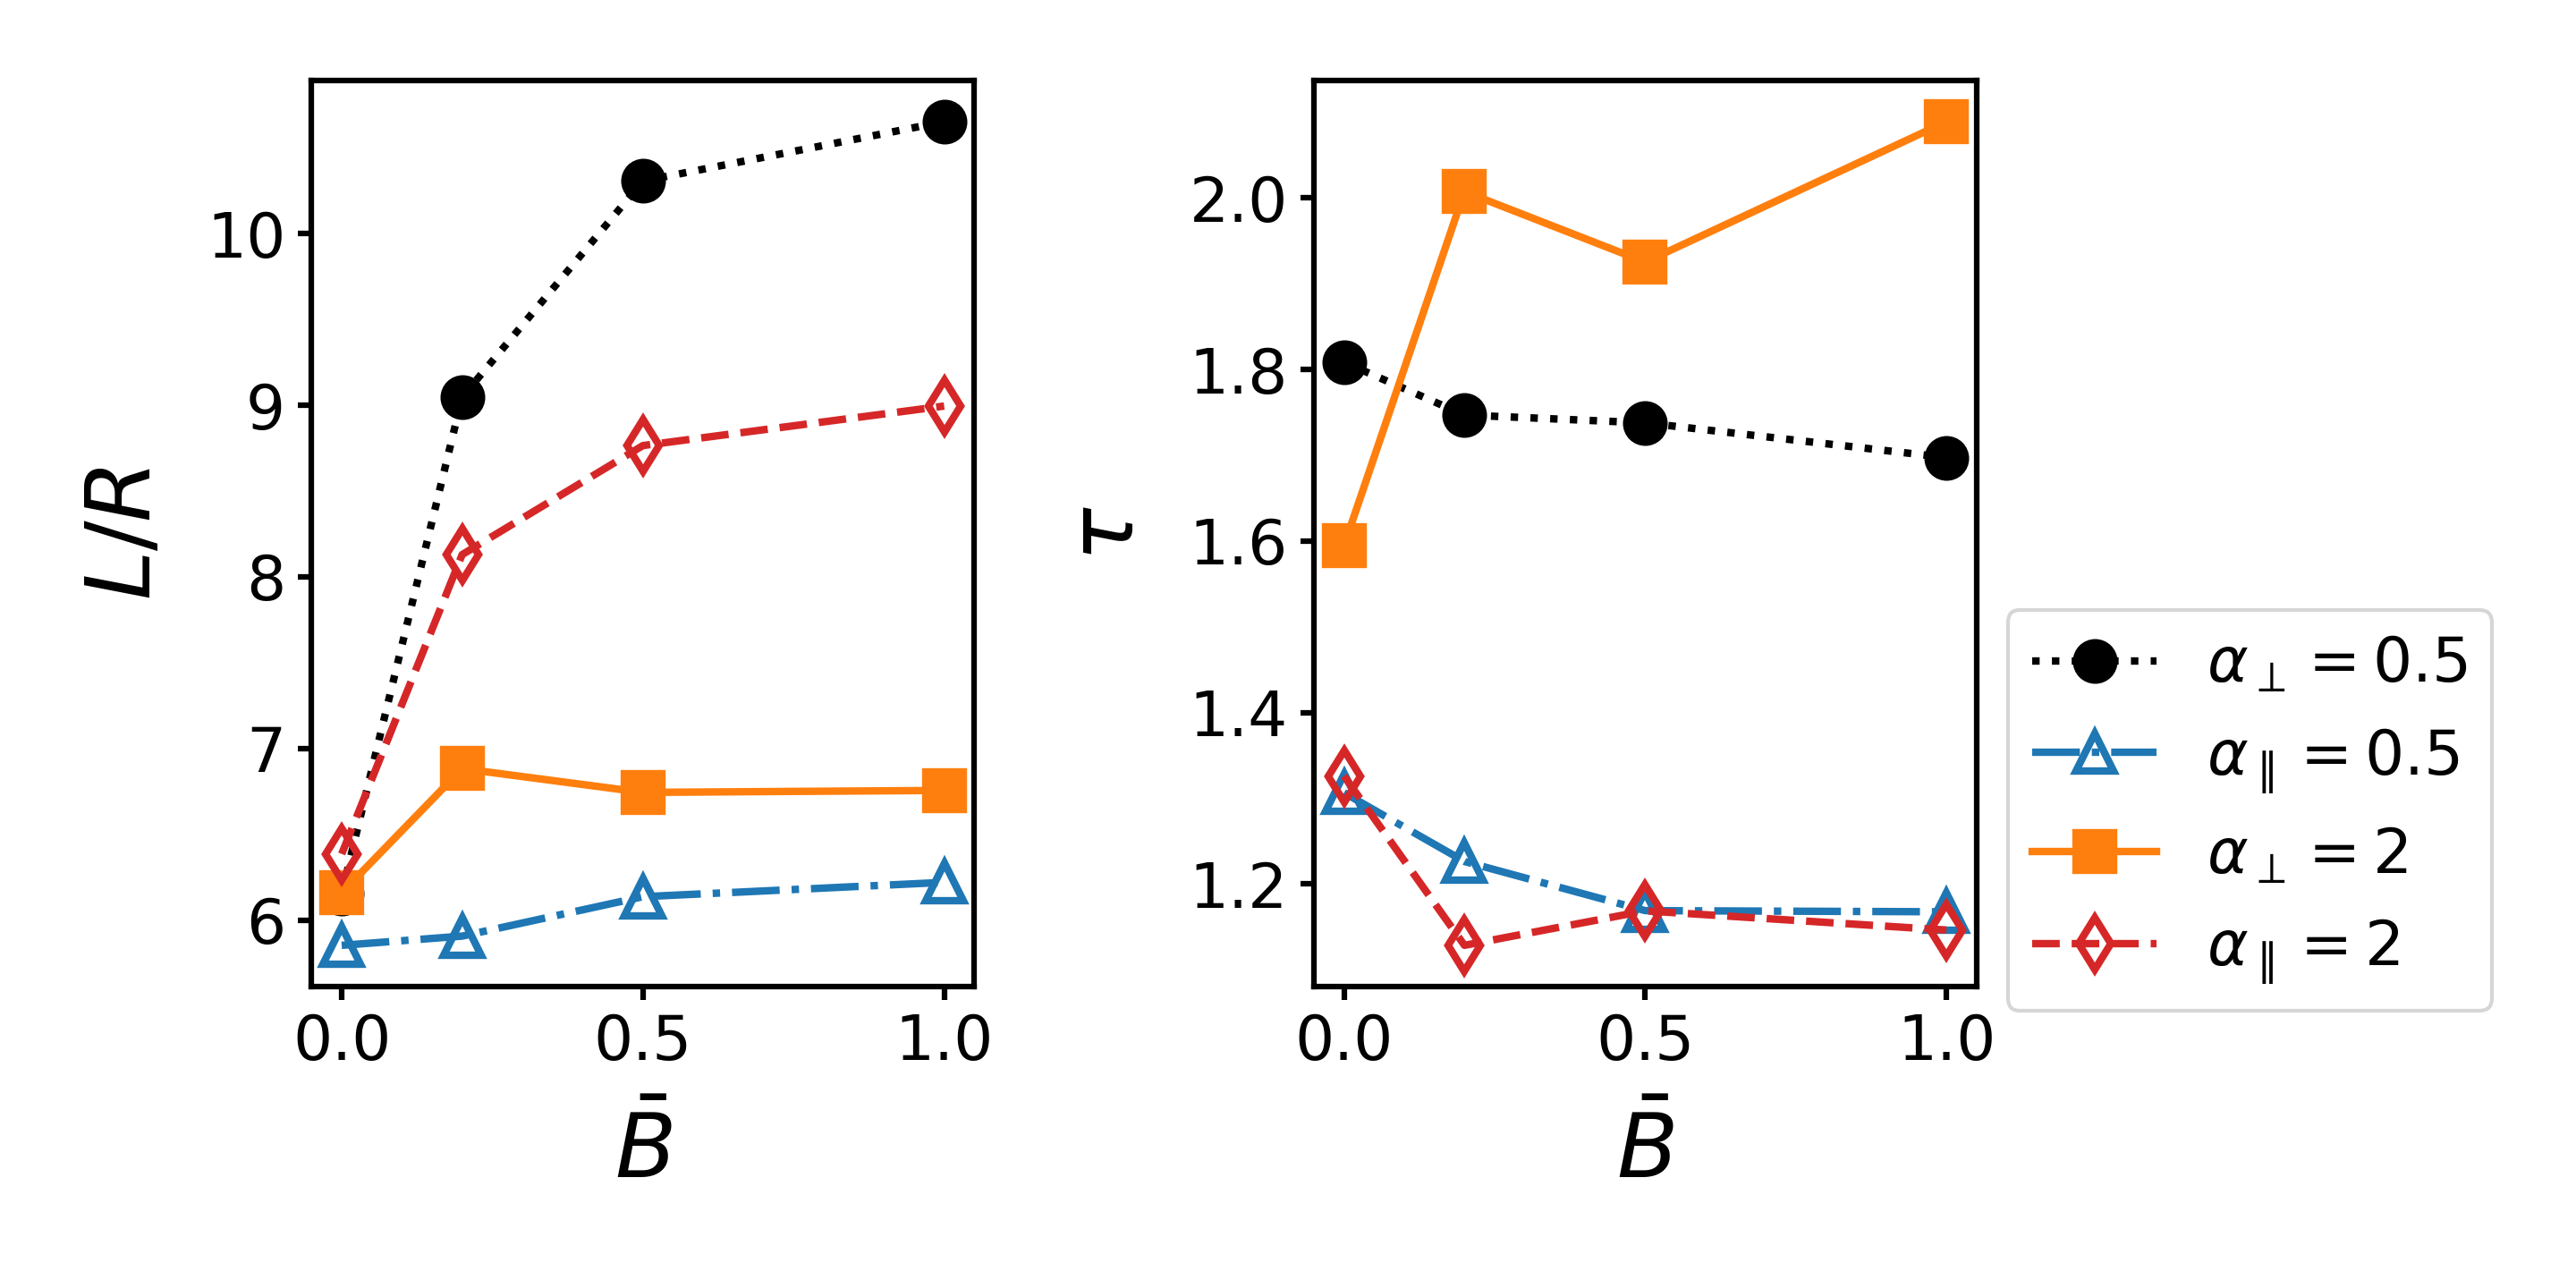
\includegraphics[scale=0.6]{../figures/results/paper2/domain_size_aniso-field_on.png} 
    \caption{Plots of the anisotropic domain size (left) and tortuosity (right) as a function of magnetic field strength for bijels 
             stabilized with oblate and prolate ellipsoids when raising the applied magnetic field. Prolate-stabilized bijels 
             exhibit increased domain size parallel to the field ($L_{\parallel}$) and decreased size perpendicular ($L_{\perp}$), 
             while the opposite trend is observed for oblate-stabilized systems. Tortuosity inversely correlates with domain size in 
             both cases.} 
    \label{fig:domain_size_aniso-field_on} 
\end{figure}

Figure~\ref{fig:domain_size_aniso-field_on} shows that the application of a magnetic field induces clear domain size anisotropy in bijels stabilized by both oblate 
and prolate particles. Even at zero field, a small degree of anisotropy is observed, which increases substantially with rising field strength. For oblate particles, 
the domain sizes perpendicular (\(L_\perp\)) and parallel (\(L_\parallel\)) to the applied field increase by approximately 73\% and 7\%, respectively. In contrast, 
for prolate particles, \(L_\perp\) increases by 10\%, while \(L_\parallel\) increases by 44\%. These results indicate that the dominant direction of coarsening 
depends on particle morphology: oblate particles promote greater coarsening perpendicular to the field, while prolate particles favor coarsening parallel to the 
field. This trend is consistent with previous findings and reflects how particles reorient in response to the applied magnetic field. As particles unjam and rejam 
at the interface, they adopt morphology- and field-dependent orientations that result in directionally biased surface coverage, manifesting as anisotropic domain 
growth.

The right panel of Figure~\ref{fig:domain_size_aniso-field_on} presents the corresponding changes in directional tortuosity. Initially, the tortuosity values 
for both directions are close to \(\tau \approx 1.5\), aligning with previous simulations of gyroidal and co-continuous structures using Lattice Boltzmann methods 
\cite{luo_macroscopic_2020}. Upon applying the magnetic field, \(\tau_\perp\) decreases while \(\tau_\parallel\) increases. This inverse relationship between 
tortuosity and domain size is consistent with prior findings \cite{karthikeyan_formation_2024}, where larger domains exhibited 
reduced tortuosity. The observed anisotropic response suggests that magnetic fields not only influence interfacial particle orientation but also lead to 
direction-dependent transport pathways in the bijel. Moreover, the extent and direction of anisotropy are strongly influenced by the particle morphology, 
particularly the axis of symmetry, which dictates the dominant direction of microstructural reorganization under field application.

Thus far, three key particle-scale phenomena have been characterized in response to the application of a magnetic field. The first is
particle alignment to the field direction, where both oblate and prolate ellipsoids reorient their major axes along the magnetic field vector. The second effect is
changes in particle tilt relative to the fluid interface, reflected in variations of the interface angle \(\langle \psi \rangle\), indicating out of interface 
reorientation driven by magnetic torque. Third, reorganization of the local particle monolayer, as captured by the evolution of the Steinhardt bond order parameter 
\(\langle Q_6 \rangle\), which reflects field-dependent disruptions and recoveries in particle ordering at the interface. Together, these processes 
drive the unjamming of the particle monolayer, causing coarsening of the fluid domains before the interface rejams in place with anisotropy dictated by the orientation
of particles to the magnetic field.

\subsection{Increasing the applied field onto a bijel made with a magnetic field}
\subsubsection{Field strength dependence on domain size}
\label{section:increasing-the-applied-field}


The hysteresis curve presented earlier in Figure~\ref{fig:hysteresis_curve} revealed that microstructural changes diminish 
with each successive increase in magnetic field strength. This saturation behavior suggests a direct link between the extent of domain coarsening 
and the evolving order within the interfacial particle monolayer. As demonstrated in the previous section, once the bijel is jammed, further domain 
growth is constrained by local rearrangements of the particles at the interface, which are themselves influenced by the degree of particle alignment 
and packing. To investigate this relationship further, we now examine how pre-existing particle order, established during bijel formation, affects 
the system's responsiveness to a subsequent applied magnetic field.

Specifically, we prepare bijel templates by applying magnetic fields of strength \(\bar{B}_{\text{template}} = 0, 0.2, 0.5, 1.0\) during the phase separation 
process, thereby generating structures stabilized by ellipsoidal particles with varying initial degrees of interfacial order. A constant magnetic field of 
\(\bar{B}_z = 1.0\) is then applied to each system post-jamming, and we monitor the microstructure evolution over a simulation duration of \(t = 10^5\) 
timesteps. For clarity, we adopt simplified notation in the discussion that follows—for example, \(\bar{B}_z: 0.0 \rightarrow 1.0\) denotes a bijel 
formed without a field and then subjected to a field of \(\bar{B}_z = 1.0\) during the response phase. We begin by qualitatively assessing the 
structural changes induced in bijels formed with different levels of initial particle ordering, as shown in Figure~\ref{fig:microstructure_viz-field_up}.

\begin{figure}
\centering 
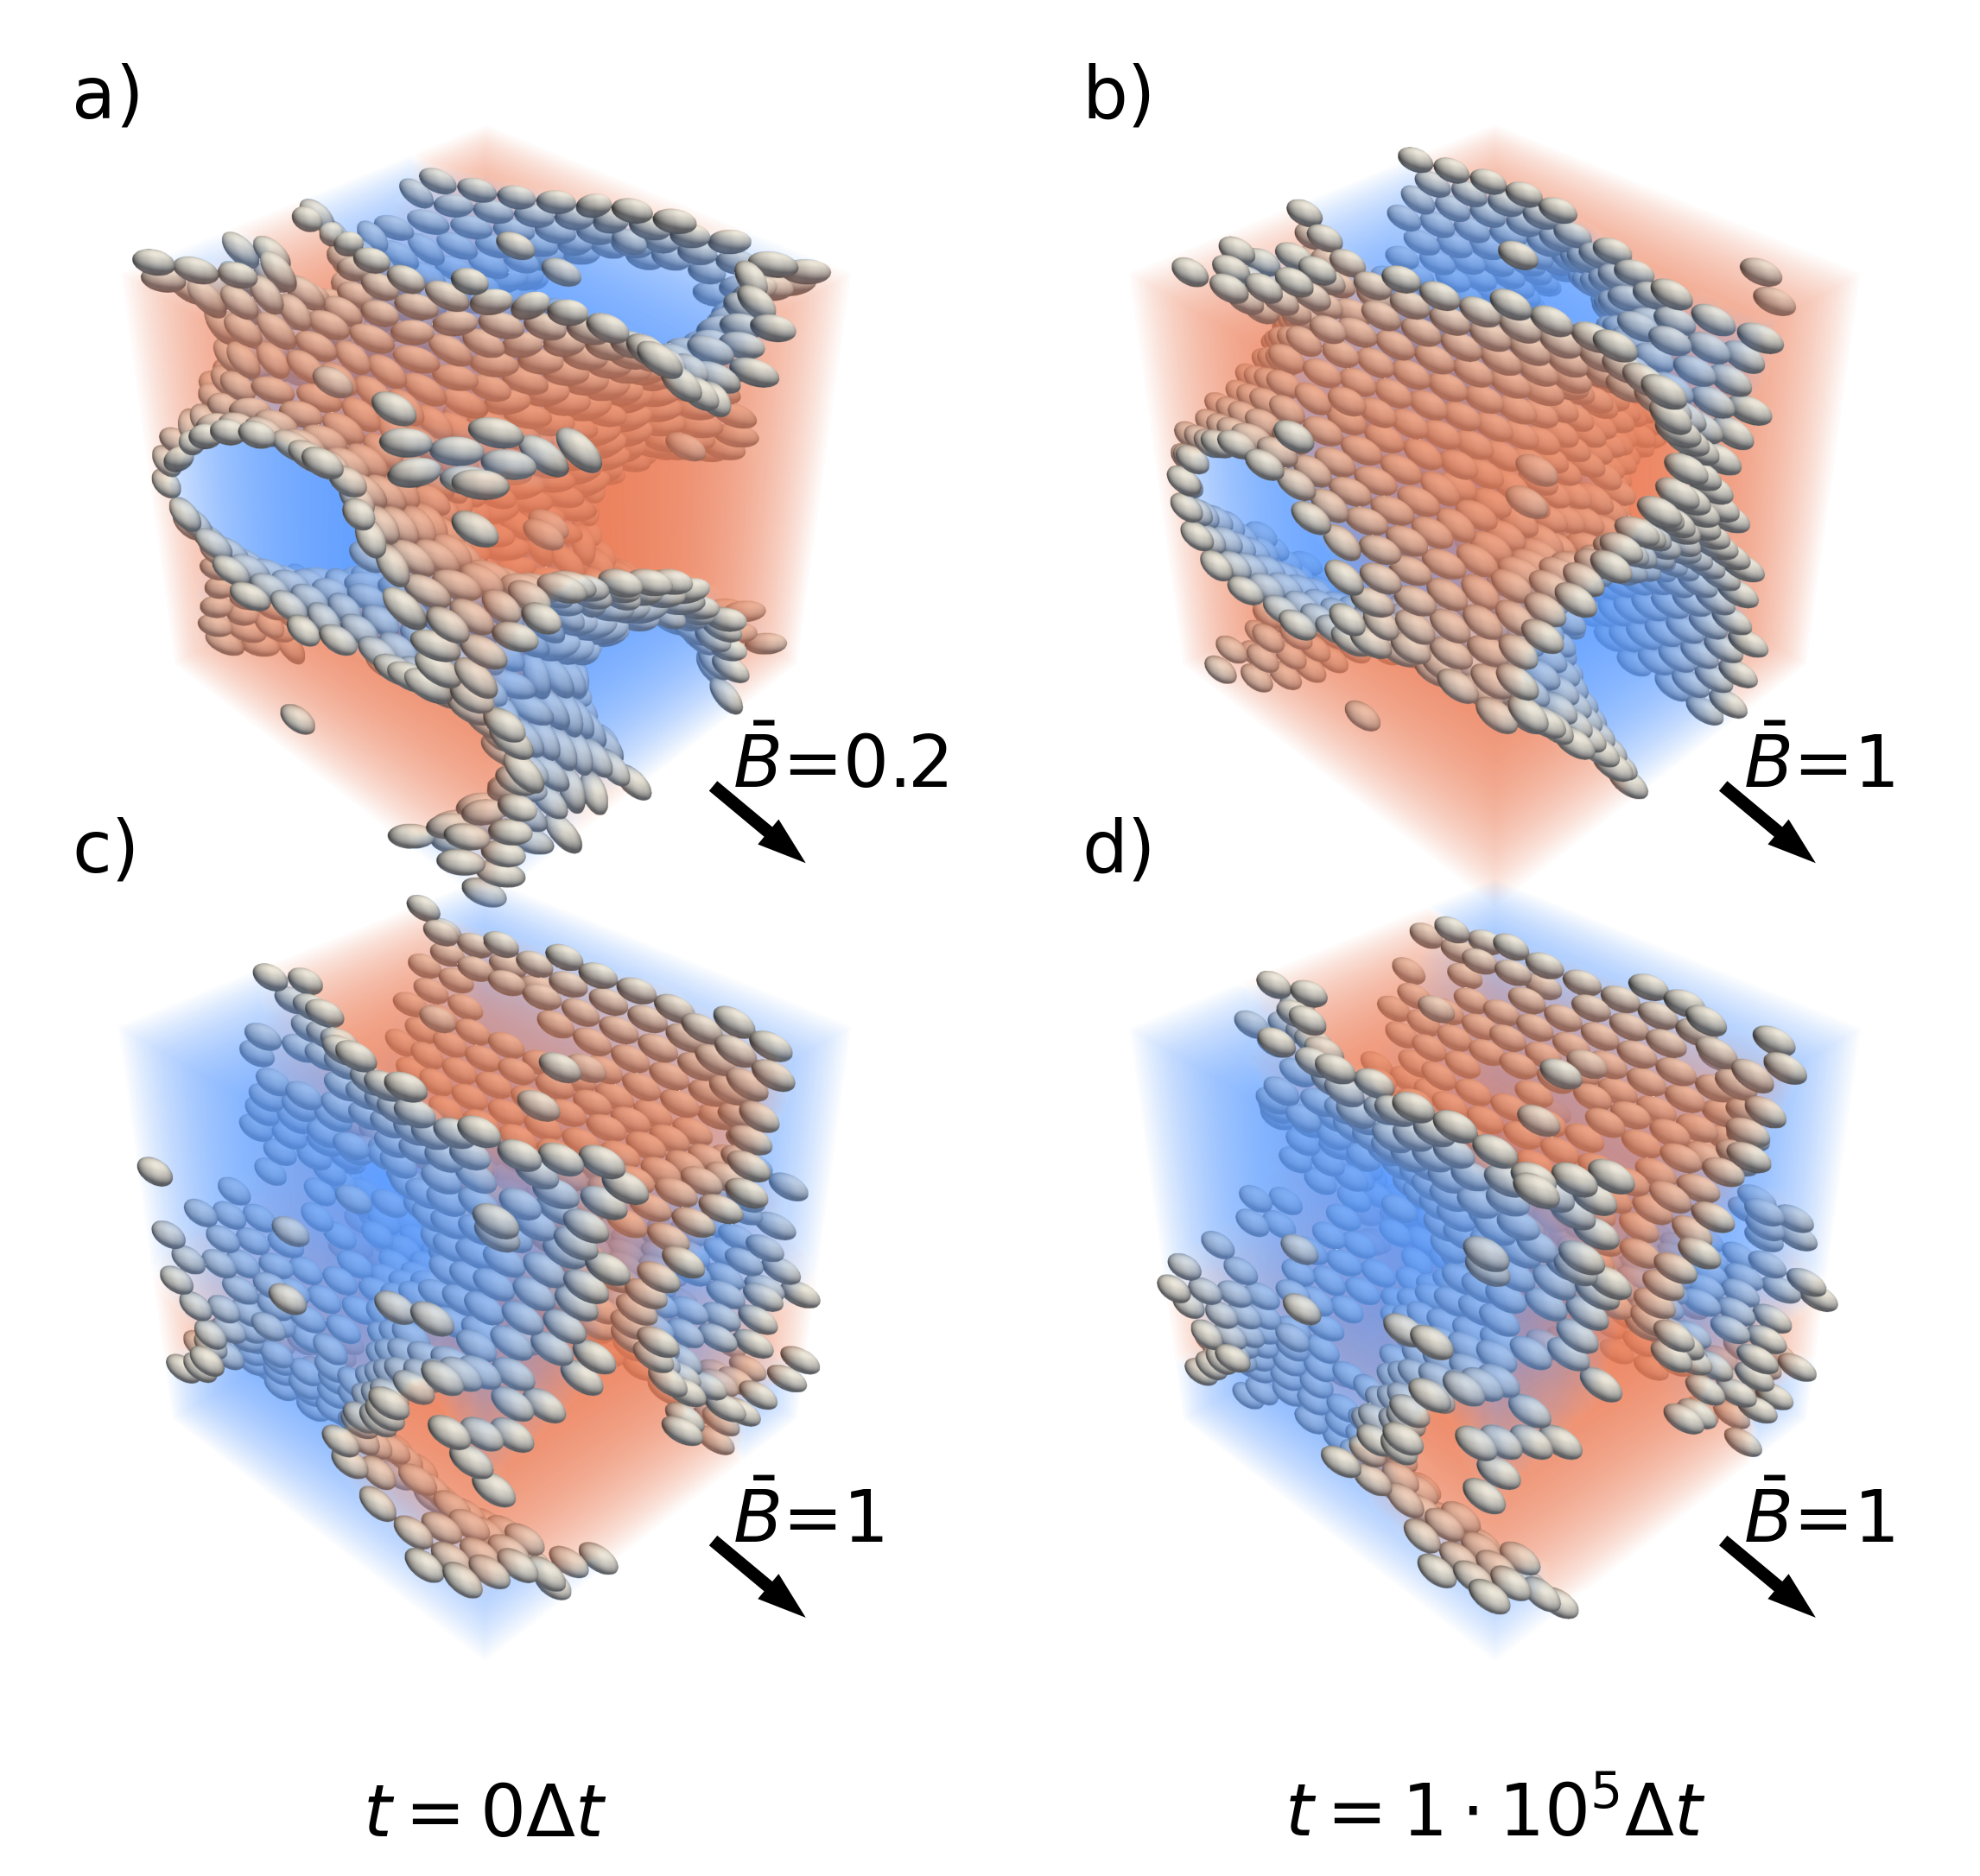
\includegraphics[scale=0.6]{../figures/results/paper2/microstructure_viz-field_up.png} 
\caption{Visualizations of bijels stabilized by prolate ellipsoidal particles at the initial (left column) and final (right column)
         timepoints for two magnetic field conditions. The top row corresponds to the case where the field is increased from 
         \(\bar{B}_z = 0.2\) to \(\bar{B}_z = 1.0\), while the bottom row shows a bijel formed and evolved under a constant field of 
         \(\bar{B}_z = 1.0\). }
\label{fig:microstructure_viz-field_up}
\end{figure}

Figure \ref{fig:microstructure_viz-field_up} demonstrates a clear initial microstructure dependent structural response, 
where the extent of domain coarsening and anisotropy is greater 
in the system that undergoes a field increase. In the \(\bar{B}_z: 0.2 \rightarrow 1.0\) case, fluid domains exhibit more pronounced reorganization and growth 
compared to the \(\bar{B}_z: 1.0 \rightarrow 1.0\) case, where the structure remains largely unchanged over time.
Additionally, a qualitative increase in particle alignment with the field direction is observed in the top row, indicating that pre-existing particle order 
limits the extent of reorientation and structural evolution under further field application. These results suggest that the degree of microstructural change 
is influenced by the difference between the initial and final magnetic field strengths, and by the capacity of the interfacial particles to reorient at the interface. 
We quantify these trends in the following section by analyzing the time evolution of domain size and the nematic order parameter in 
Figure~\ref{fig:domain_size-field_up}.

\begin{figure} 
\centering 
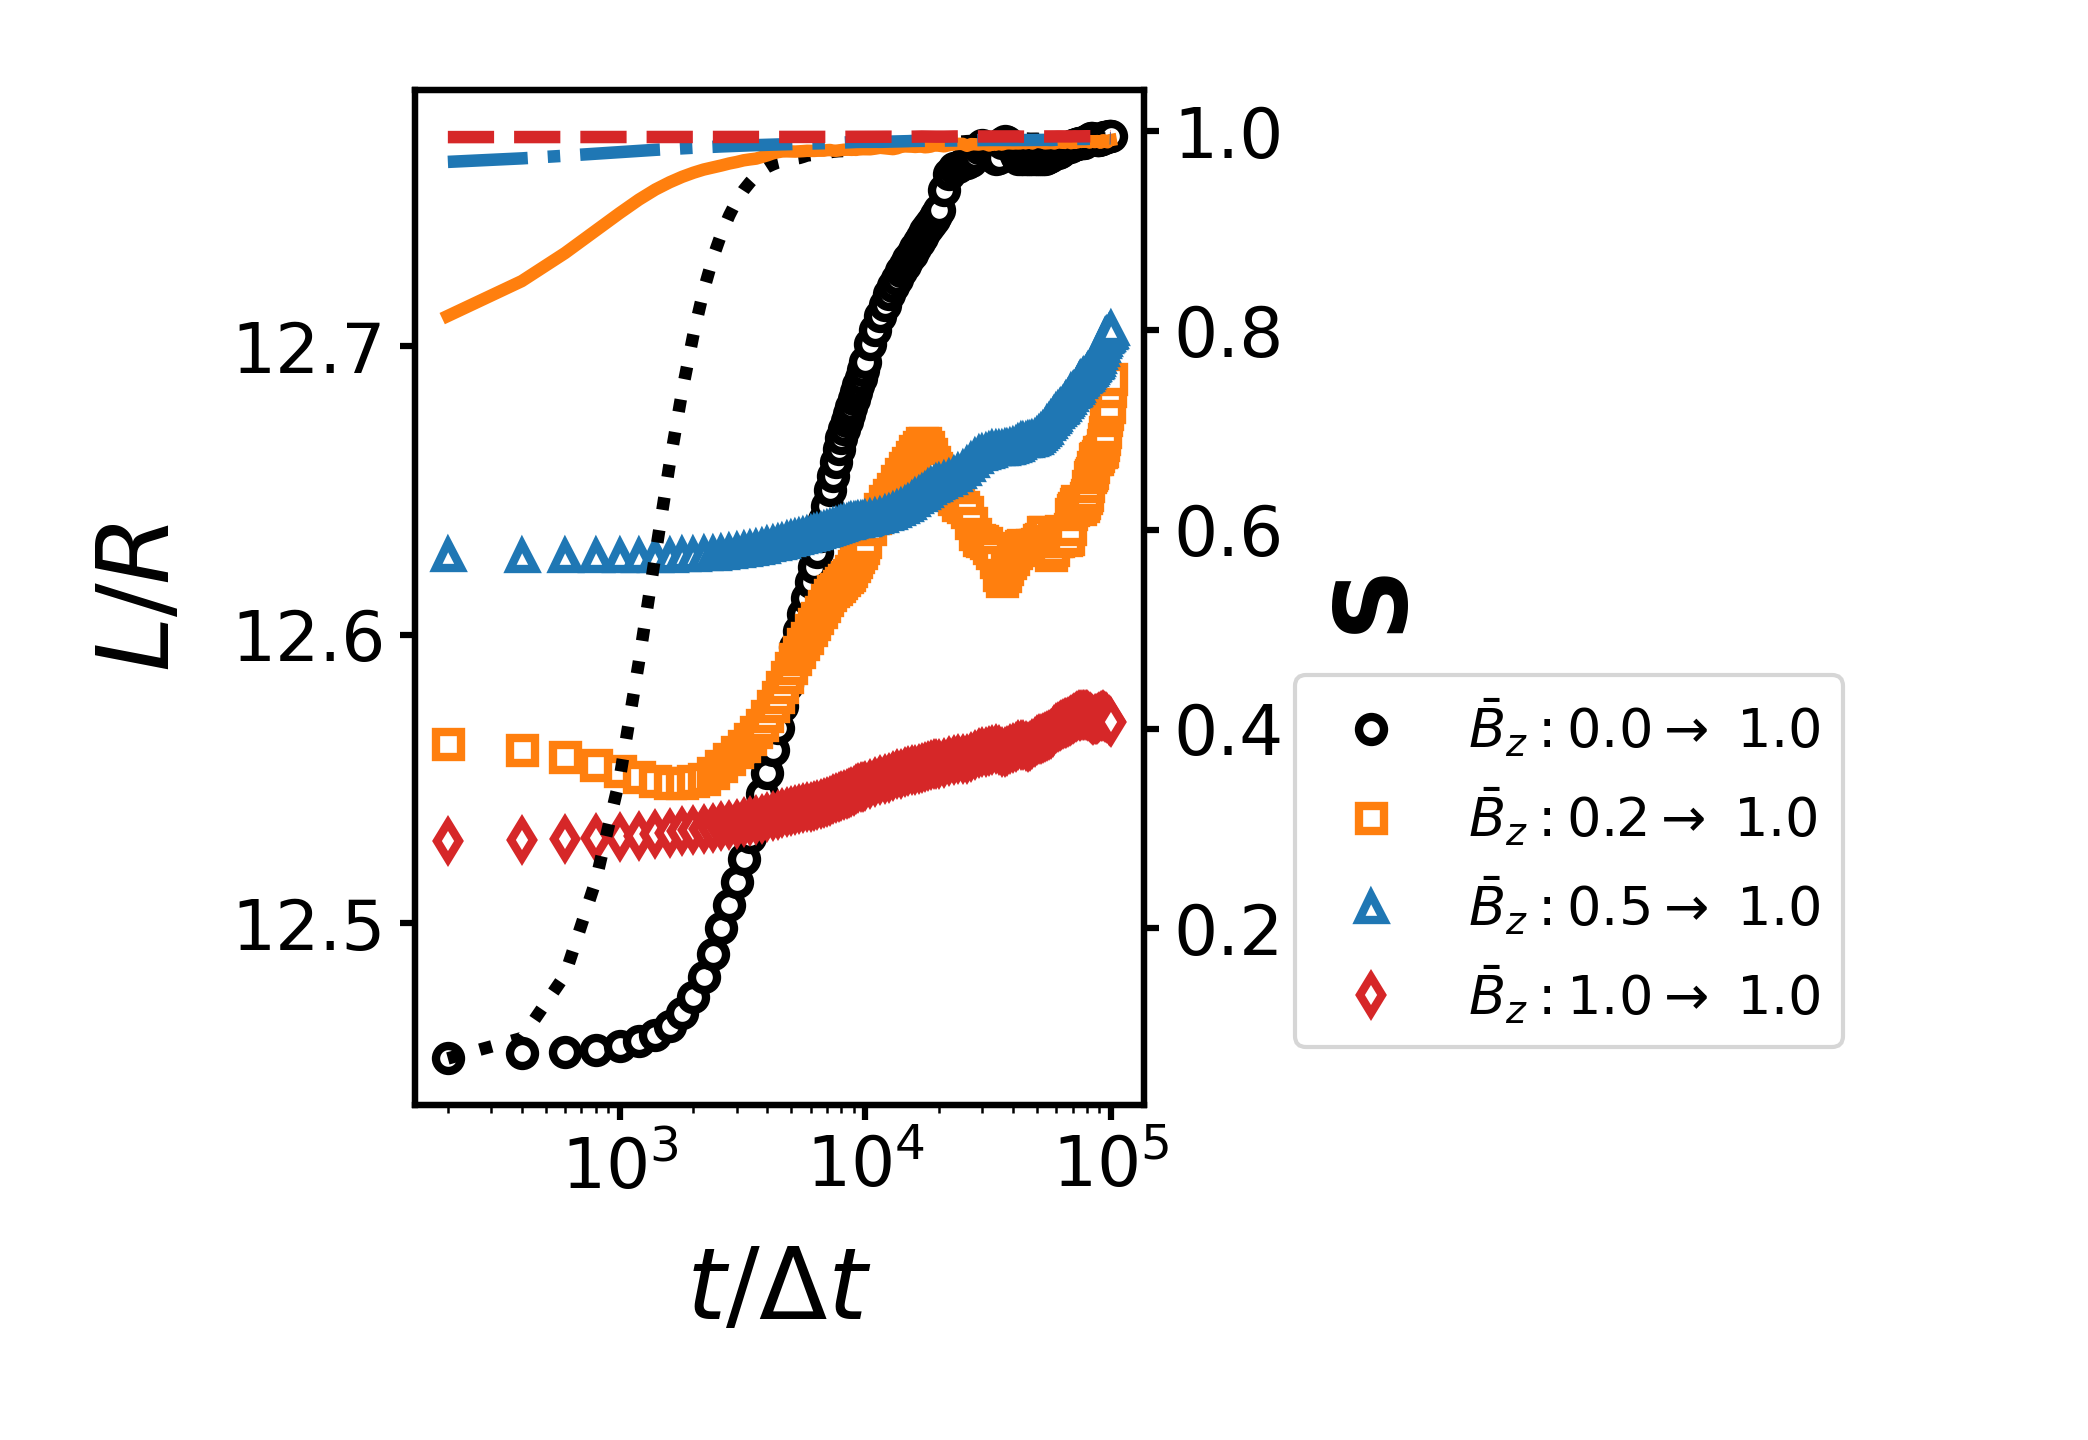
\includegraphics[scale=0.6]{../figures/results/paper2/domain_size-field_up.png} 
\caption{Plot of the spherically averaged domain size normalized with $Rp(L/R)$ of the particle in markers and the nematic order parameter in lines. 
         We show that the domain size change measured is correlated to the change in the particle ordering, characterized using the nematic order parameter.} 
\label{fig:domain_size-field_up} 
\end{figure}

Figure~\ref{fig:domain_size-field_up} presents the evolution of domain size \(L/R\) and nematic order parameter \(S\) for bijels stabilized by oblate (left) 
and prolate (right) particles under various field transition conditions. We define \(\Delta \bar{B}\) as the difference between the final and initial magnetic 
field strengths. The onset and magnitude of the microstructural response are both observed to be dependent on \(\Delta \bar{B}\), indicating that a stronger 
magnetic field change provides a greater driving force for structural reorganization. Specifically, when \(\Delta \bar{B} = 1.0\), the resulting domain size 
increases by approximately 5\% for oblate particles and 2\% for prolate particles. These structural changes diminish progressively as \(\Delta \bar{B}\) decreases.

The accompanying nematic order parameter \(S\) also correlates strongly with \(\Delta \bar{B}\), suggesting that domain size evolution is intrinsically linked 
to the extent of particle alignment within the system. Higher values of \(\Delta \bar{B}\) induce greater particle reorientation, which facilitates is linked to
reconfiguration of particles at the interface, thereby enabling domain coarsening. These findings highlight that characteristic length scale evolution is jointly 
governed by both particle aspect ratio and the magnitude of magnetic field variation. To further quantify anisotropic changes in microstructure, we define the 
relative change in directional domain size as \(\Delta L = \frac{L_f - L_i}{L_i}\), where \(L\) refers to either \(L_{\perp}\) or \(L_{\parallel}\). 
The same formulation is applied to the directional tortuosity components. These metrics allow us to isolate and characterize the \(\Delta \bar{B}\)-dependent 
evolution of anisotropic structural features. The results are presented and analyzed in Figure~\ref{fig:domain_size_aniso-field_up}.

\begin{figure} 
\centering 
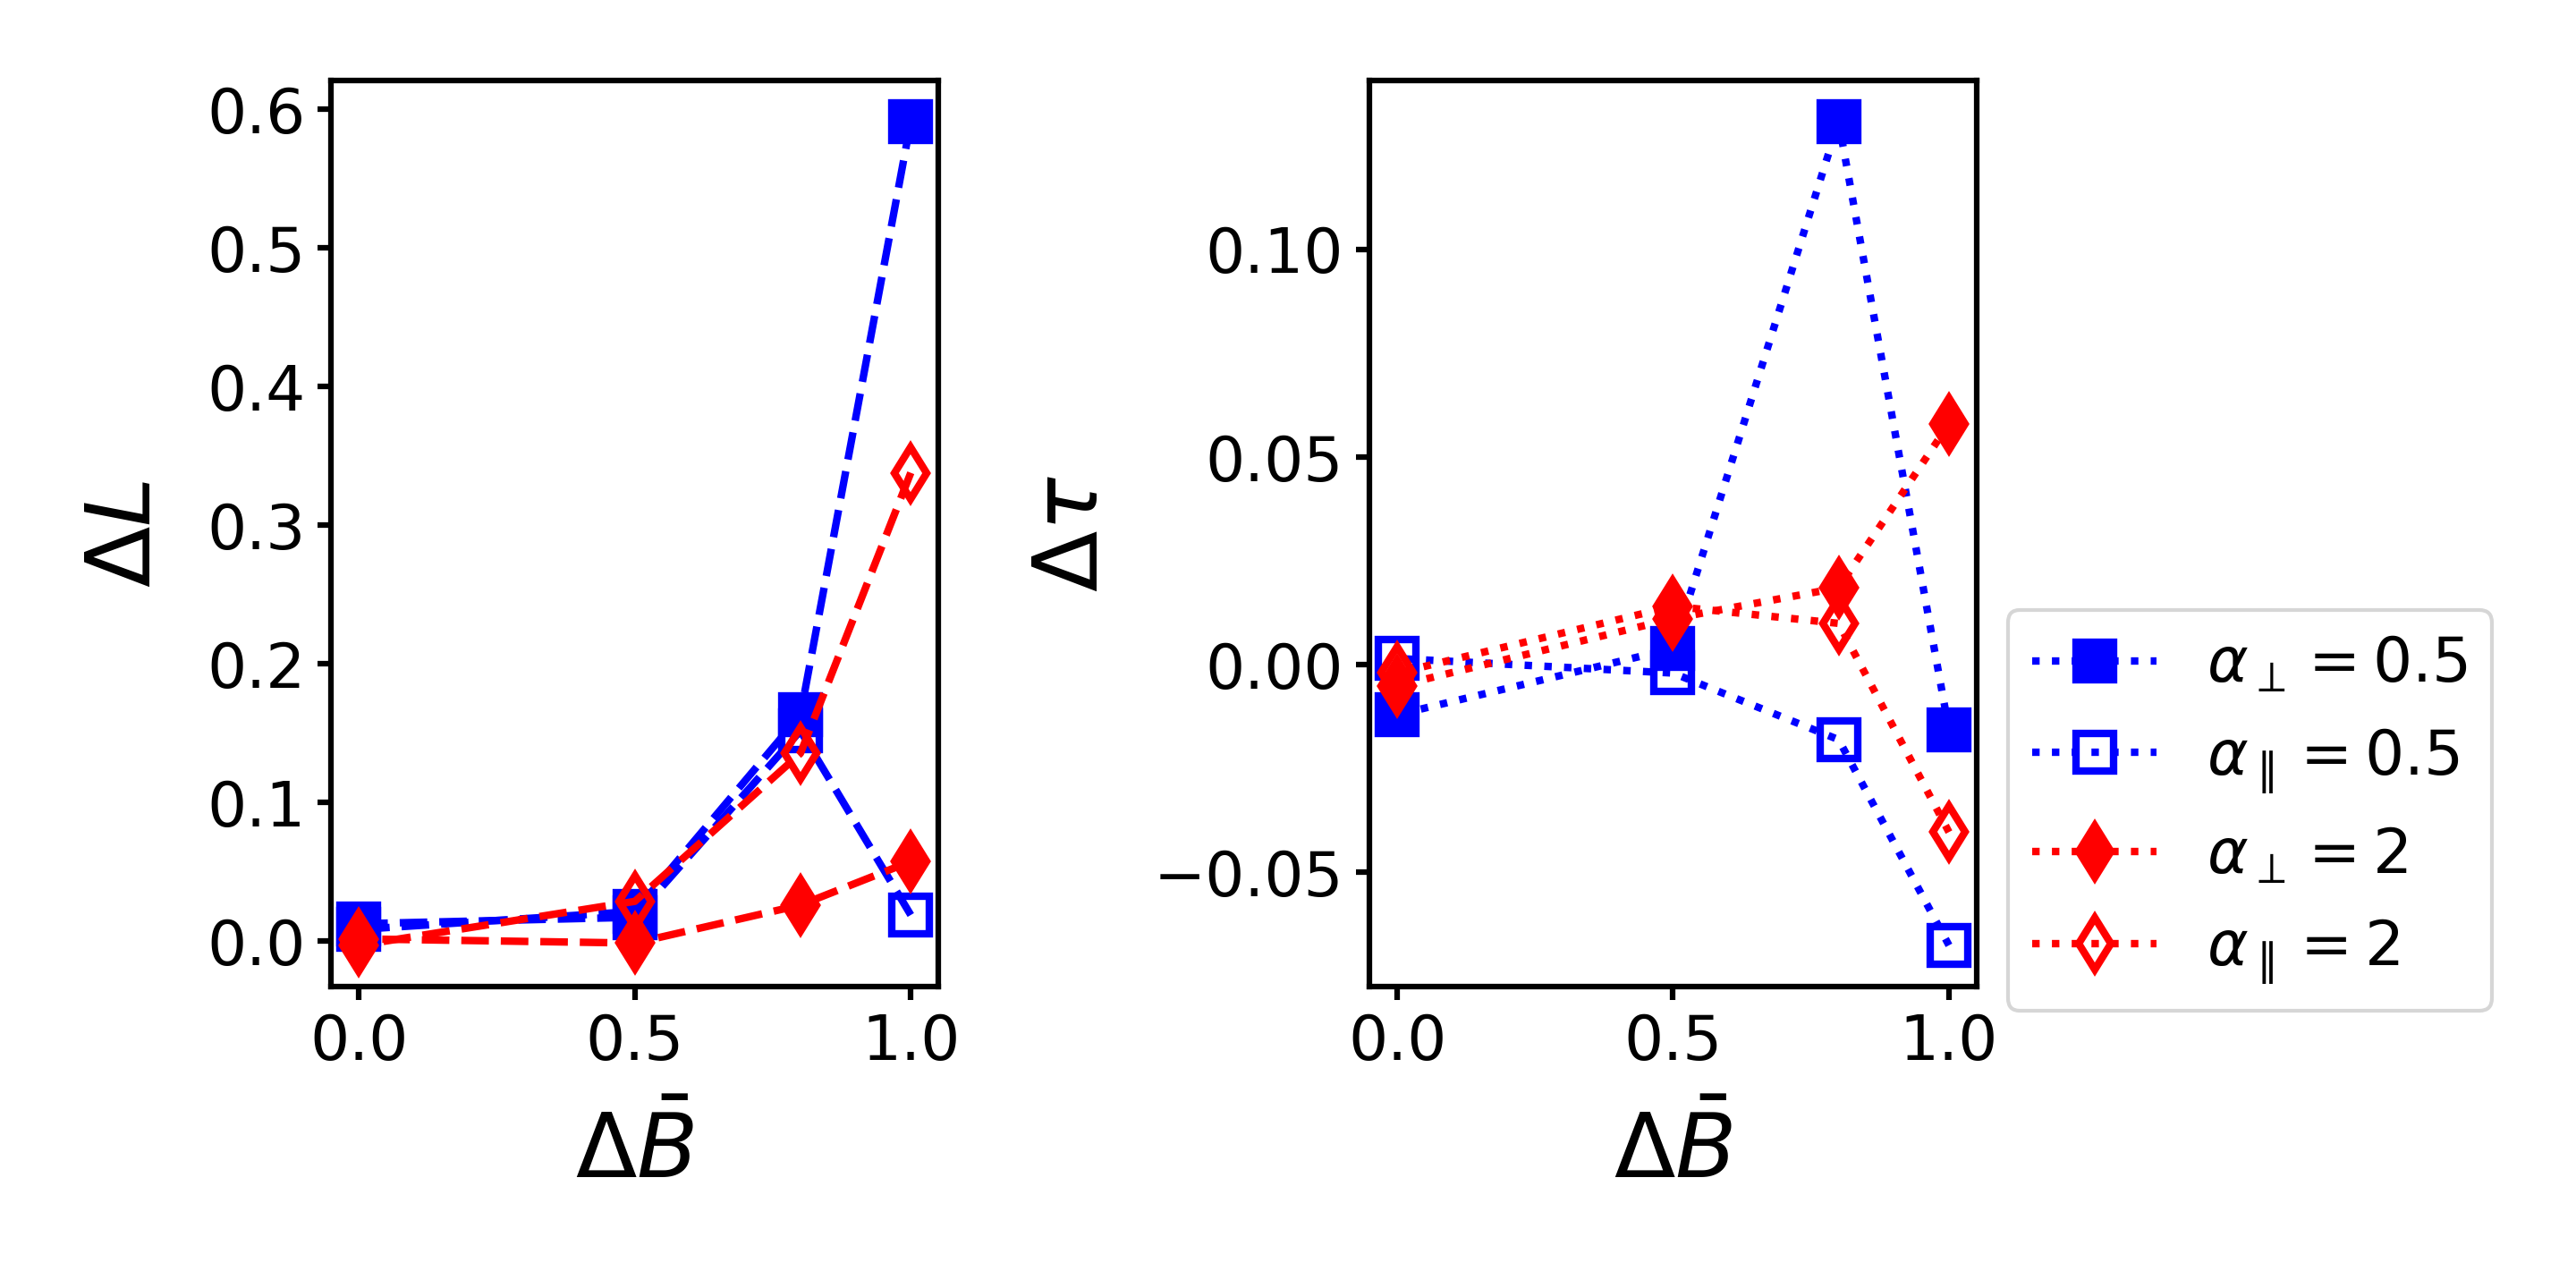
\includegraphics[scale = 0.6]{../figures/results/paper2/domain_size_aniso-field_up.png} 
\caption{Plotting the anisotropic domain sizes and tortuosity at the final timestep on the left and right respectively for bijels stabilized with 
         oblate and prolate ellipsoidal particles starting at different particle orders. We plot these results against the change in the applied field 
         strength, $\Delta B$. The anisotropic domain size is inversely correlated to the tortuosity and $L_{perp}$ changes for 
         a bijel made with $\bar{B} = 1 \rightarrow 1$ and $\bar{B}: 0 \rightarrow 1$ differ, suggesting that the processing history of the bijel is important.} 
\label{fig:domain_size_aniso-field_up} 
\end{figure}

Figure~\ref{fig:domain_size_aniso-field_up} quantifies the directional changes in domain size (\(\Delta L\)) and tortuosity (\(\Delta \tau\)) as a 
function of magnetic field variation \(\Delta \bar{B}\), for bijels stabilized by oblate (blue) and prolate (red) particles. The results show that 
increasing the applied magnetic field leads to enhanced domain size anisotropy in both particle systems. Even in the absence of a magnetic field 
change (\(\Delta \bar{B} = 0\)), a small degree of anisotropy is observed, which becomes more pronounced as \(\Delta \bar{B}\) increases. For oblate 
particles, the perpendicular and parallel domain sizes increase by approximately 73\% and 7\%, respectively. In contrast, for prolate particles, the 
increases are 10\% and 44\%, respectively. The direction of dominant coarsening aligns with prior findings and reflects how particles reorient under 
the influence of the magnetic field—oblate particles tend to reorient and promote coarsening perpendicular to the field, while prolate particles favor 
coarsening along the field direction.

The right panel shows the corresponding changes in directional tortuosity. The initial tortuosity is approximately \(\tau \approx 1.5\), consistent with 
Lattice Boltzmann simulations of gyroid and co-continuous porous structures \cite{luo_macroscopic_2020}. Upon field application, \(\tau_\perp\) 
generally decreases while \(\tau_\parallel\) increases, in agreement with the observed domain size changes. These trends are consistent with prior 
work \cite{karthikeyan_formation_2024}, which demonstrated an inverse relationship between domain size and tortuosity. The results confirm that 
magnetic field-driven domain anisotropy significantly affects the transport properties of the bijel, with particle shape and orientation playing a 
critical role in determining the direction and magnitude of these structural changes. The shape of the plots indicate that the decrease in structural response
is correlated strongly to an increase in the ordering of the particles. In the next section, we focus more on the particle monolayer.

\subsubsection{Particle reorientation as a function of initial particle order}

The results presented thus far demonstrate that the extent of microstructural evolution, particularly domain anisotropy and coarsening, decreases sharply 
as the difference between the initial and final magnetic field strengths (\(\Delta \bar{B}\)) approaches zero. This exponential decay in structural 
response suggests that beyond a certain threshold, the system becomes increasingly resistant to reorganization. Since domain-scale changes are driven 
by local particle rearrangements at the interface, this diminishing response points to a progressively reduced capacity of the particle monolayer to 
unjam and reorient under small field perturbations. To better understand the origin of this resistance to structural change, we now shift our focus to 
the particle monolayer itself. Specifically, we examine how initial ordering within the interfacial particle layer governs the system's ability to respond 
to further magnetic stimuli.

\begin{figure} 
\centering 
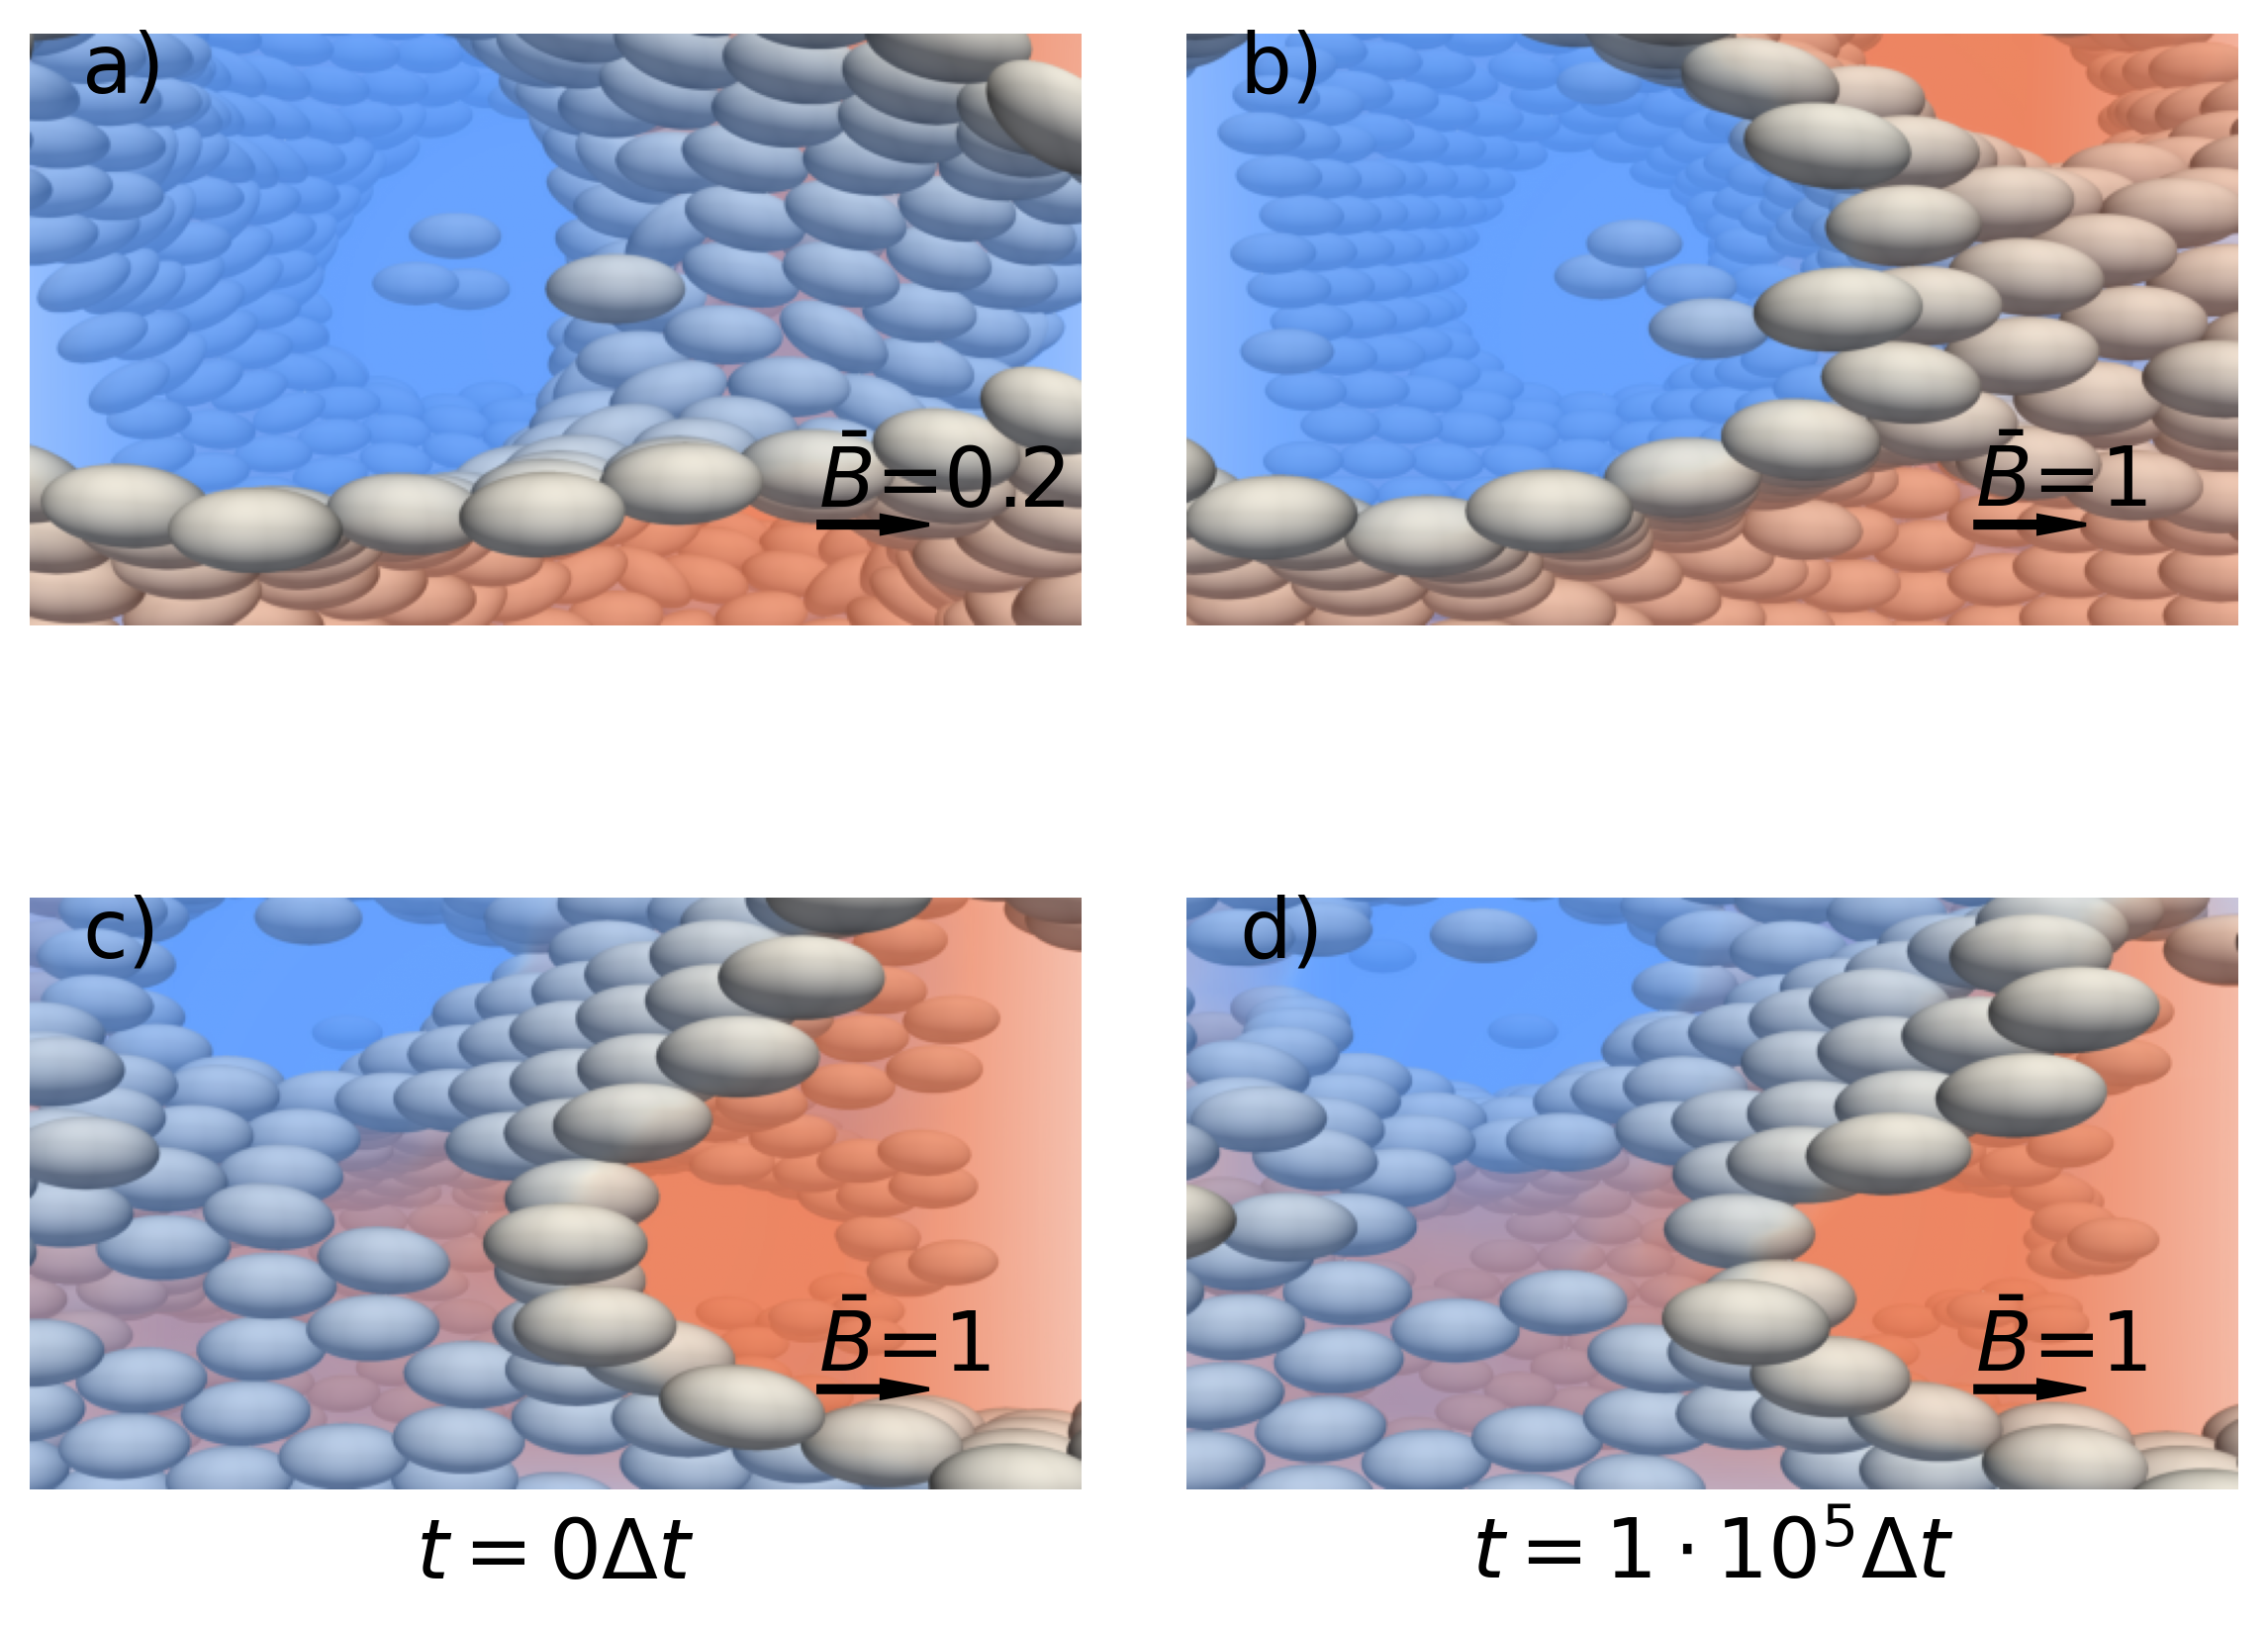
\includegraphics[scale=0.5]{../figures/results/paper2/particle_viz-field_up.png} 
\caption{Snapshots of the structural evolution of the particle monolayer in bijels stabilized by prolate ellipsoids 
         under different magnetic field conditions. The top row corresponds to a simulation where the field is increased from 
         \(\bar{B} = 0.2\) to \(\bar{B} = 1.0\), while the bottom row shows a system maintained at a constant field of \(\bar{B} = 1.0\) throughout.} 
\label{fig:particle_viz-field_up} 
\end{figure}

Even at the initial timepoint of the \(\bar{B}: 0.2 \rightarrow 1.0\) run, a majority of particles are already aligned with the field direction. 
Upon increasing the field strength to \(\bar{B} = 1.0\), nearly all visible particles exhibit strong alignment, consistent with the high nematic order 
parameter values observed in Figure~\ref{fig:domain_size-field_up}.
The visual alignment of the particles long axes with the magnetic field highlights the mechanism driving anisotropic domain formation in the bijel. 
As particle orientation is locked in by magnetic torque, the interfacial arrangement becomes directionally biased, influencing the resulting domain 
morphology. To quantitatively link this particle-scale reorientation to the observed structural anisotropy, we next evaluate the average interface 
angle \(\langle \psi \rangle\) in Figure \ref{fig:interface_angle-field_on}

\begin{figure} 
    \centering 
    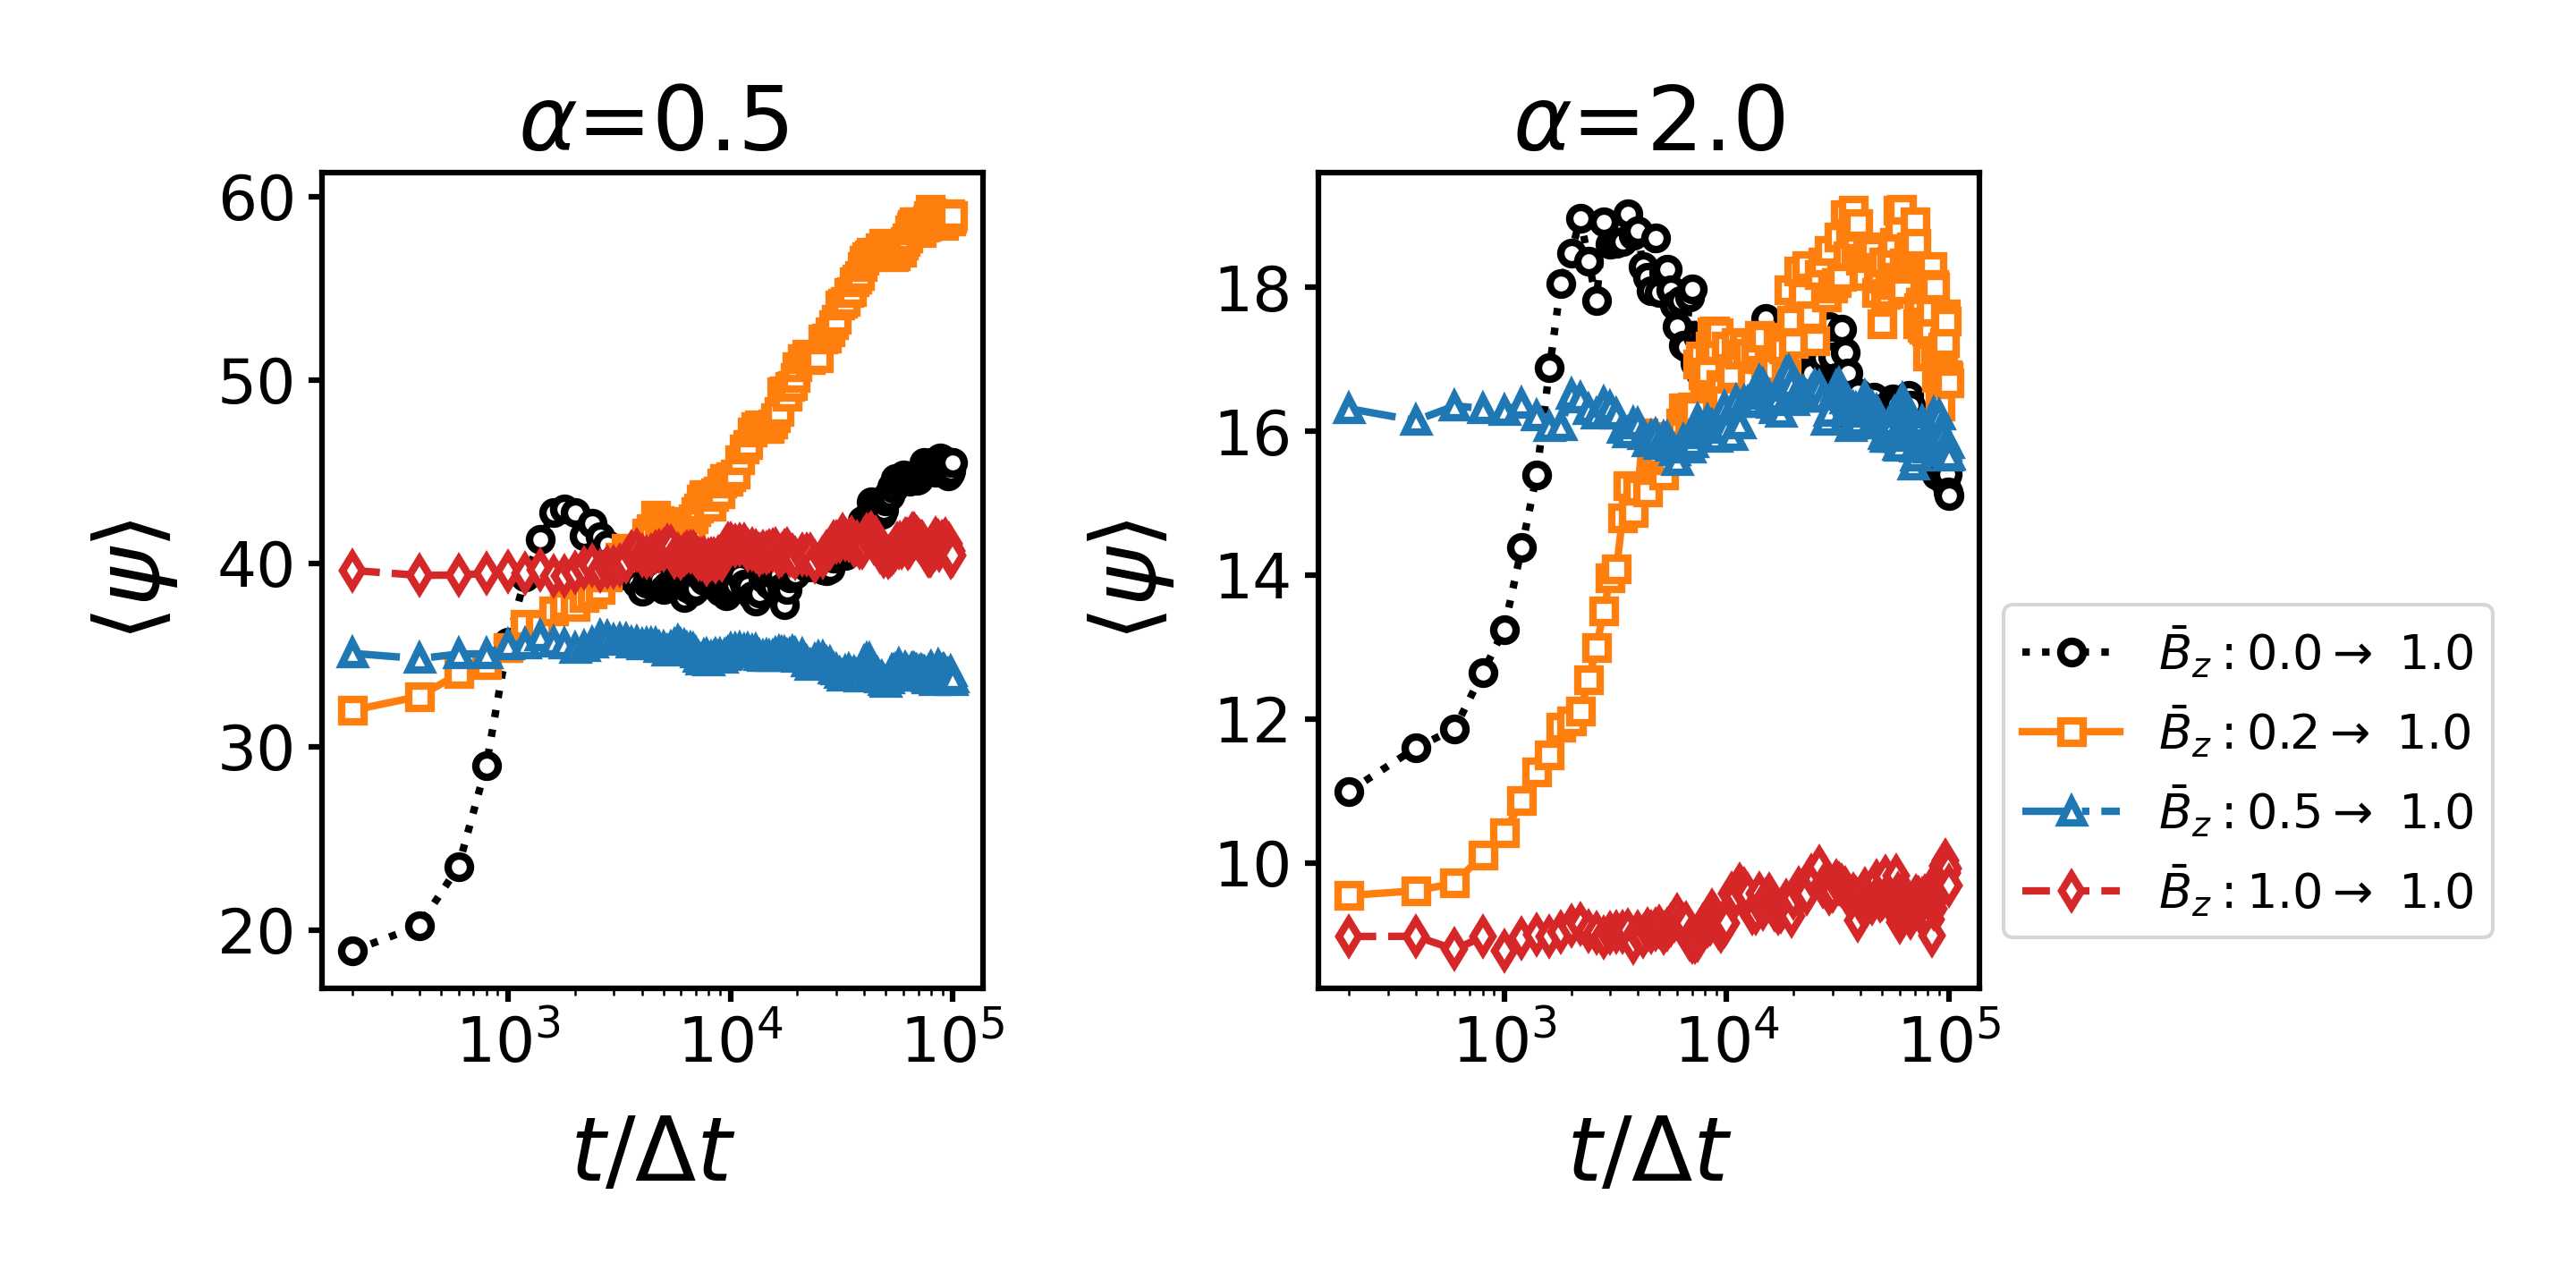
\includegraphics[scale=0.6]{../figures/results/paper2/psi-field_up.png} 
    \caption{Plots of the evolution of the average interface angle \(\langle \psi \rangle\) for bijels stabilized 
             by oblate (left) and prolate (right) particles, as a function of the initial microstructure and subsequent magnetic field application.
             The dynamics observed can be seen to be a function of the initial microstructure.} 
    \label{fig:interface_angle-field_up} 
\end{figure}

The results show that the initial particle ordering plays a significant role in the interfacial response. As characterized earlier for the case of
$\bar{B}:0.0 \rightarrow 1.0$ the time evolution of $\langle \psi \rangle$ has three stages characterized as a rapid increase, followed by a plateau
and finally as jamming sets in, a slow increase or decrease. However when initial ordering is present this behavior is different. At 
$\bar{B}: 0.2 \rightarrow 1.0$, bijels stabilized by ellipsoidal particles see a gradual increase in $\langle \psi \rangle$ for both particle aspect ratios.
At stronger magnetic fields, $\bar{B}: 0.5 \rightarrow 1.0$ and $\bar{B}: 1.0 \rightarrow 1.0$, there is little to no change in $\langle \psi \rangle$ indicating
that the magnetic field has no effect on the particle monolayer. This indicates that the mechanism of structural response if beginning with an ordered particle
monolayer differs from that of a disordered one. We confirm this by plotting the Steinhardt 6 fold order parameter $\langle Q_6 \rangle$ in Figure \ref{fig:Q6-field_up}

\begin{figure} 
    \centering 
    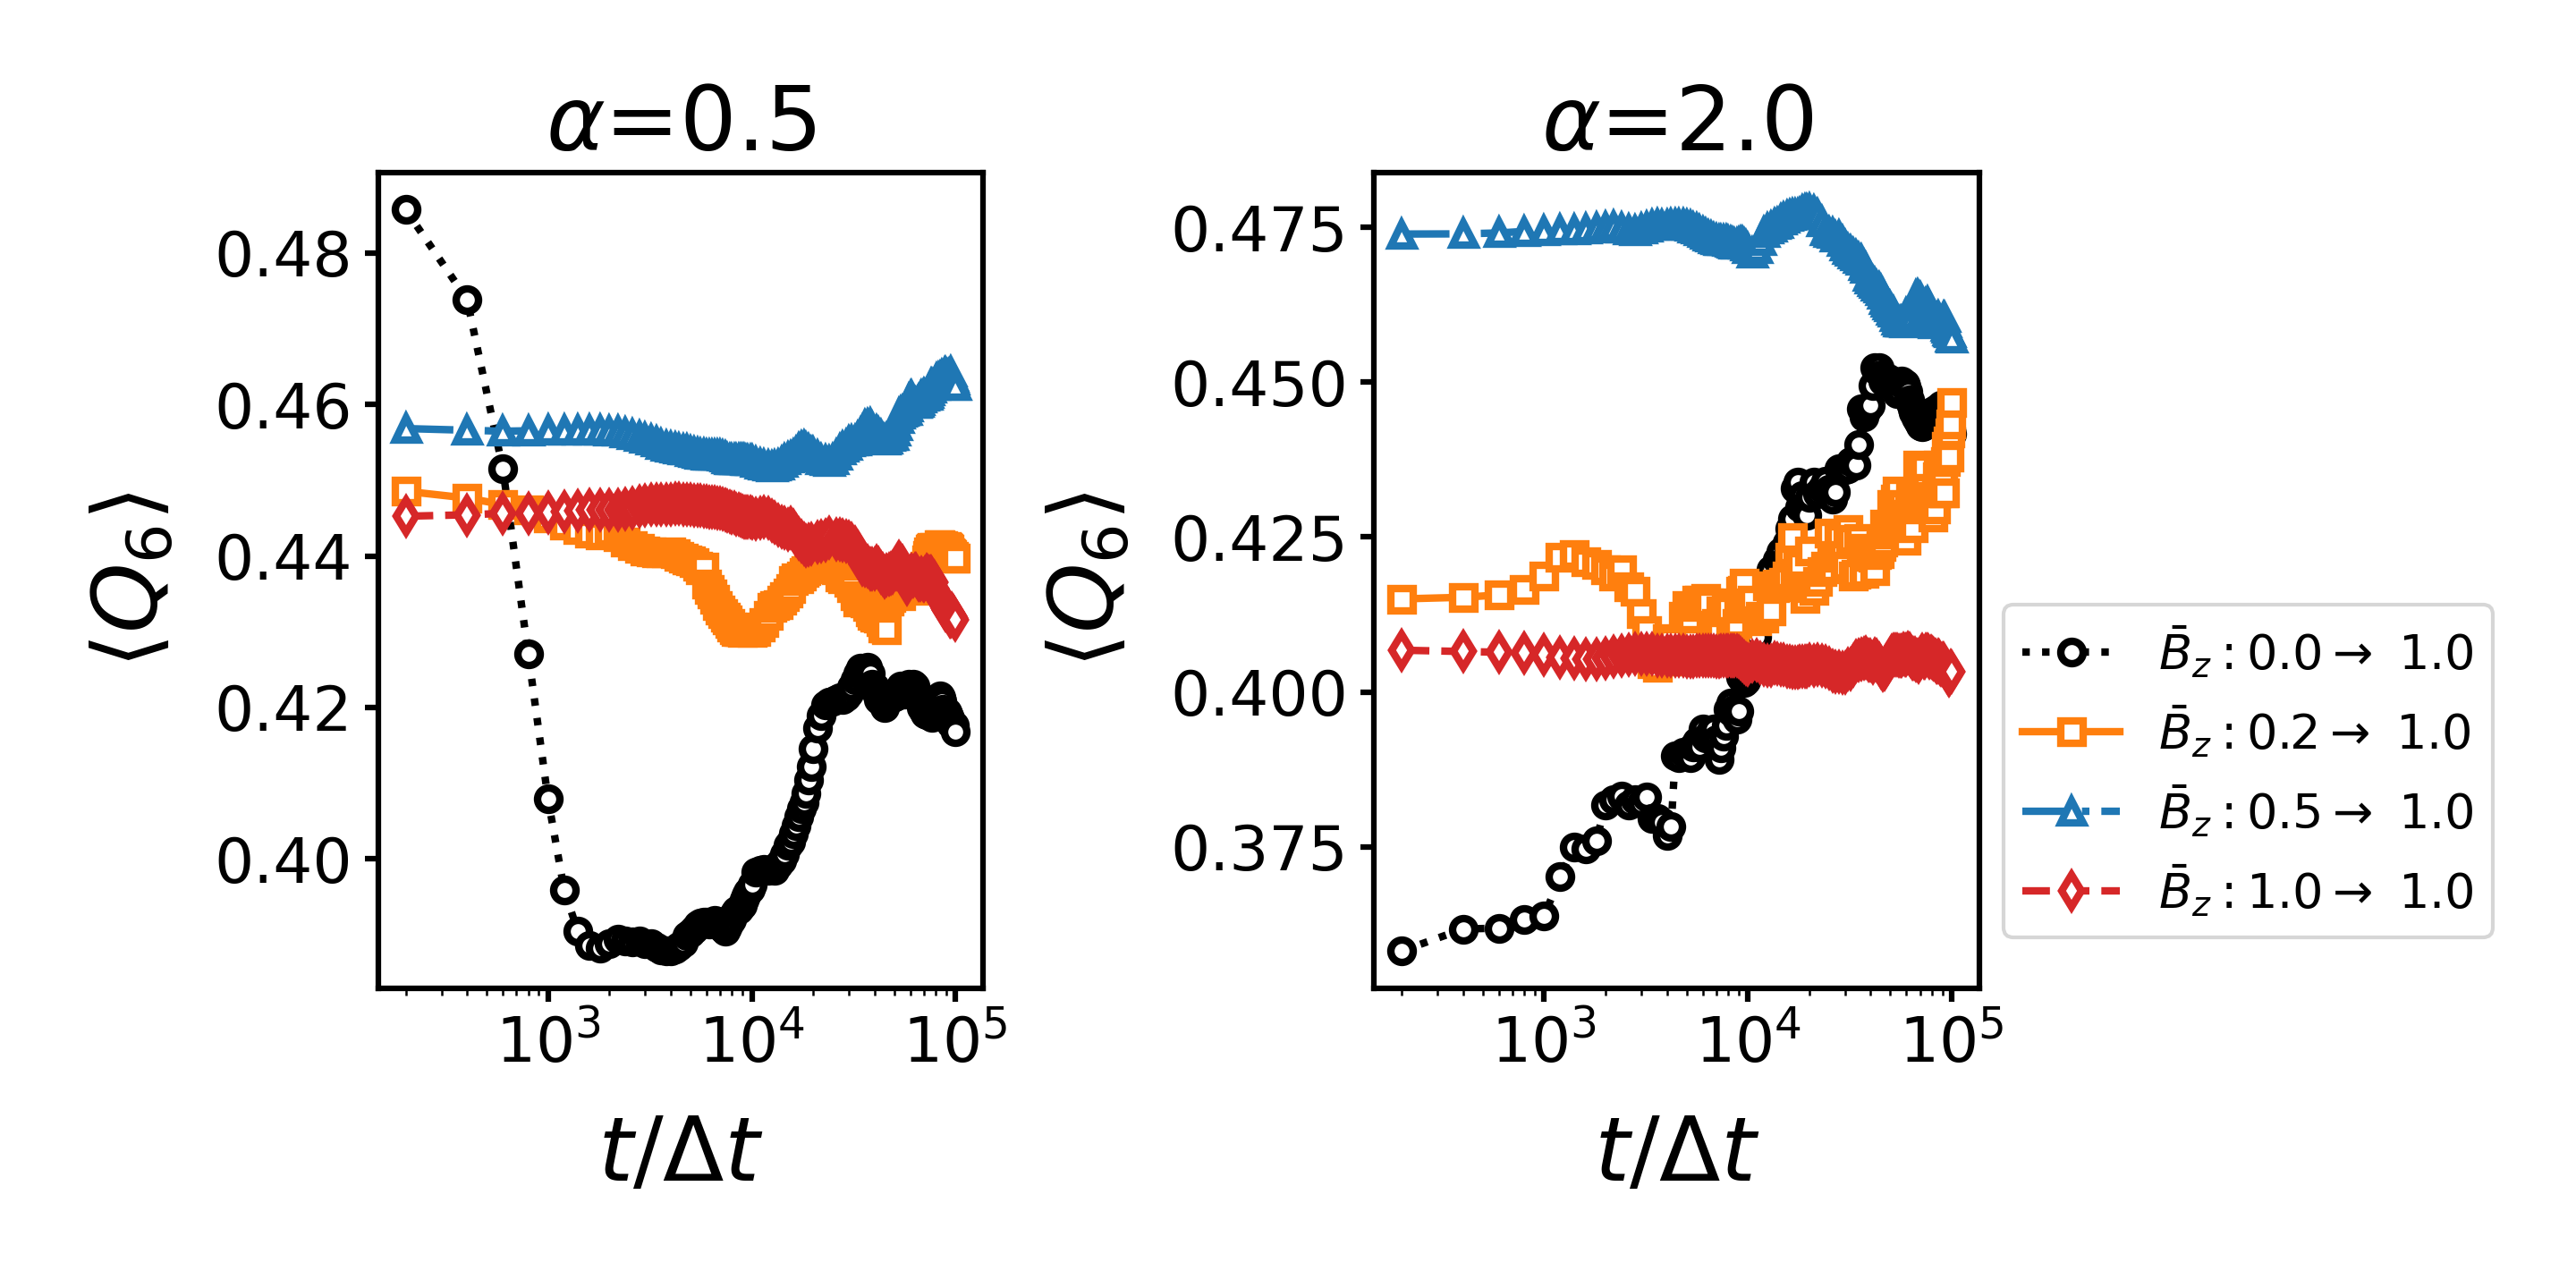
\includegraphics[scale=0.6]{../figures/results/paper2/Q6-field_up.png} 
    \caption{Plots of the evolution of the average interface angle \(\langle Q6 \rangle\) for bijels stabilized 
             by oblate (left) and prolate (right) particles, as a function of the initial microstructure and subsequent magnetic field application.
             The dynamics observed can be seen to be a function of the initial microstructure.} 
    \label{fig:Q6-field_up} 
\end{figure}

For oblate particles, both the \(\bar{B}: 0.0 \rightarrow 1.0\) and 
\(\bar{B}: 0.2 \rightarrow 1.0\) cases exhibit a three-phase progression characterized as an initial decline in \(\langle Q_6 \rangle\), followed by a 
plateau and a subsequent increase that stabilizes over time. The most pronounced decrease is observed in the \(\bar{B}: 0.0 \rightarrow 1.0\) case, where a 
highly ordered monolayer undergoes significant disruption due to the sudden field-induced reorientation of particles. The recovery of \(\langle Q_6 \rangle\) 
following this dip reflects the system's gradual reordering as particles adjust to their new orientation and repack at the interface.
For the \(\bar{B}: 1.0 \rightarrow 1.0\) system, \(\langle Q_6 \rangle\) remains nearly constant, indicating that the monolayer was already aligned and 
structurally stable at the onset of the simulation. The \(\bar{B}: 0.5 \rightarrow 1.0\) case stands out as an intermediate response, with only minor 
fluctuations in \(\langle Q_6 \rangle\), suggesting limited capacity for additional structural reorganization due to pre-existing particle alignment.

In the case of prolate particles, the behavior for systems with lower initial field values (\(\bar{B}: 0.0 \rightarrow 1.0\) 
and \(\bar{B}: 0.2 \rightarrow 1.0\)) show monotonic increases in \(\langle Q_6 \rangle\), indicating a progressive gain in local particle ordering as the 
field drives further interfacial reorganization. The magnitude and rate of increase are greatest in the \(\bar{B}: 0.0 \rightarrow 1.0\) case, which aligns with 
the larger structural transformations observed in the microstructure. In contrast, the \(\bar{B}: 1.0 \rightarrow 1.0\) case remains largely unchanged, 
confirming that the system has already reached its field-aligned state. The $\bar{B}: 0.5 \rightarrow 1.0$ shows some variations, although broadly there are no
significant changes in the interfacial arrangement. 

Taken together, the results reveal two distinct categories of structural response in magnetically responsive bijels, governed by the initial degree of particle 
ordering. The first category arises when the bijel is stabilized by a disordered particle monolayer. In this case, the application of a magnetic field drives 
particle rotation and tilting out of the interface, which reduces the available interfacial area stabilized by the particles. This destabilization initiates 
domain coarsening. As the fluid domains grow, capillary interactions couple with the evolving particle orientations, allowing the interface to deform in concert 
with the particle dynamics. Ultimately, the microstructure becomes kinetically arrested as the particles rejam in their new field-aligned configurations, leading 
to a stable, coarsened structure.

The second category corresponds to systems with an initially nematically ordered monolayer, where the director is misaligned with the magnetic field. Here, the 
applied field reorients the particles within the plane of the interface without inducing unjamming. Because the particle network remains structurally constrained, 
the interface angle increases gradually as particles rotate, but without triggering large-scale fluid reorganization. Microstructural changes in this regime are 
instead driven by localized adjustments in interfacial packing, rather than full-scale interface remodeling.  

Finally, when the particle monolayer is already well-aligned with the magnetic field direction, minimal reorientation occurs, and no significant structural 
response is observed. This finding highlights that particle reorientation—particularly when it induces or is coupled with unjamming—is a prerequisite for 
enabling dynamic microstructural evolution in bijels under magnetic fields. These insights underscore the importance of processing history and interfacial 
particle configuration in tuning bijel responsiveness for functional applications.

\subsection{Decreasing the applied field}
\label{decreasing-the-applied-field}

Bijels are kinetically arrested systems whose long-term structural properties are governed by the stability and arrangement 
of the interfacial particle monolayer. Prior studies on responsive emulsions have shown that even after the removal of external 
stimuli, the microstructure often remains unchanged for extended periods due to the interfacial 
jamming of particles \cite{cui_stabilizing_2013}. Similarly, in the hysteresis experiments 
discussed earlier (Figure~\ref{fig:hysteresis_curve}), we observed that reducing or removing the magnetic field did not 
lead to a reversal of domain coarsening or particle realignment, suggesting an inherent structural resilience once the bijel 
has stabilized.

However, bijels are formed through a dynamic arrest during spinodal decomposition, and the 
particles jam in configurations that may not correspond to a thermodynamic minimum particularly when a magnetic field is 
applied during formation. Gunther et al. also showed that bijels stabilized by ellipsoidal particles exhibited timescales 
of response distinct from bijels stabilized by spherical particle due to steric effects between ellipsoidal paticles.
Therefore, this section will seek to understand to what extent the initial particle order affects the 
bijel's capacity to relax or restructure upon removal of the field. To explore this, 
we now examine the post-stimulus structural response of bijels formed under different field conditions 
\(\bar{B}_{\text{template}} = 0.0, 0.2, 0.5, 1.0\). After allowing each structure to fully stabilize under a 
constant magnetic field, we abruptly switch off the field and observe the subsequent time evolution of both the 
microstructure and interfacial particle behavior over a duration of \(t = 10^5 \Delta t\). This analysis aims to 
clarify the mechanisms that underpin the apparent irreversibility captured in the hysteresis response and further 
assess the role of processing history in bijel stability.

\begin{figure} 
\centering 
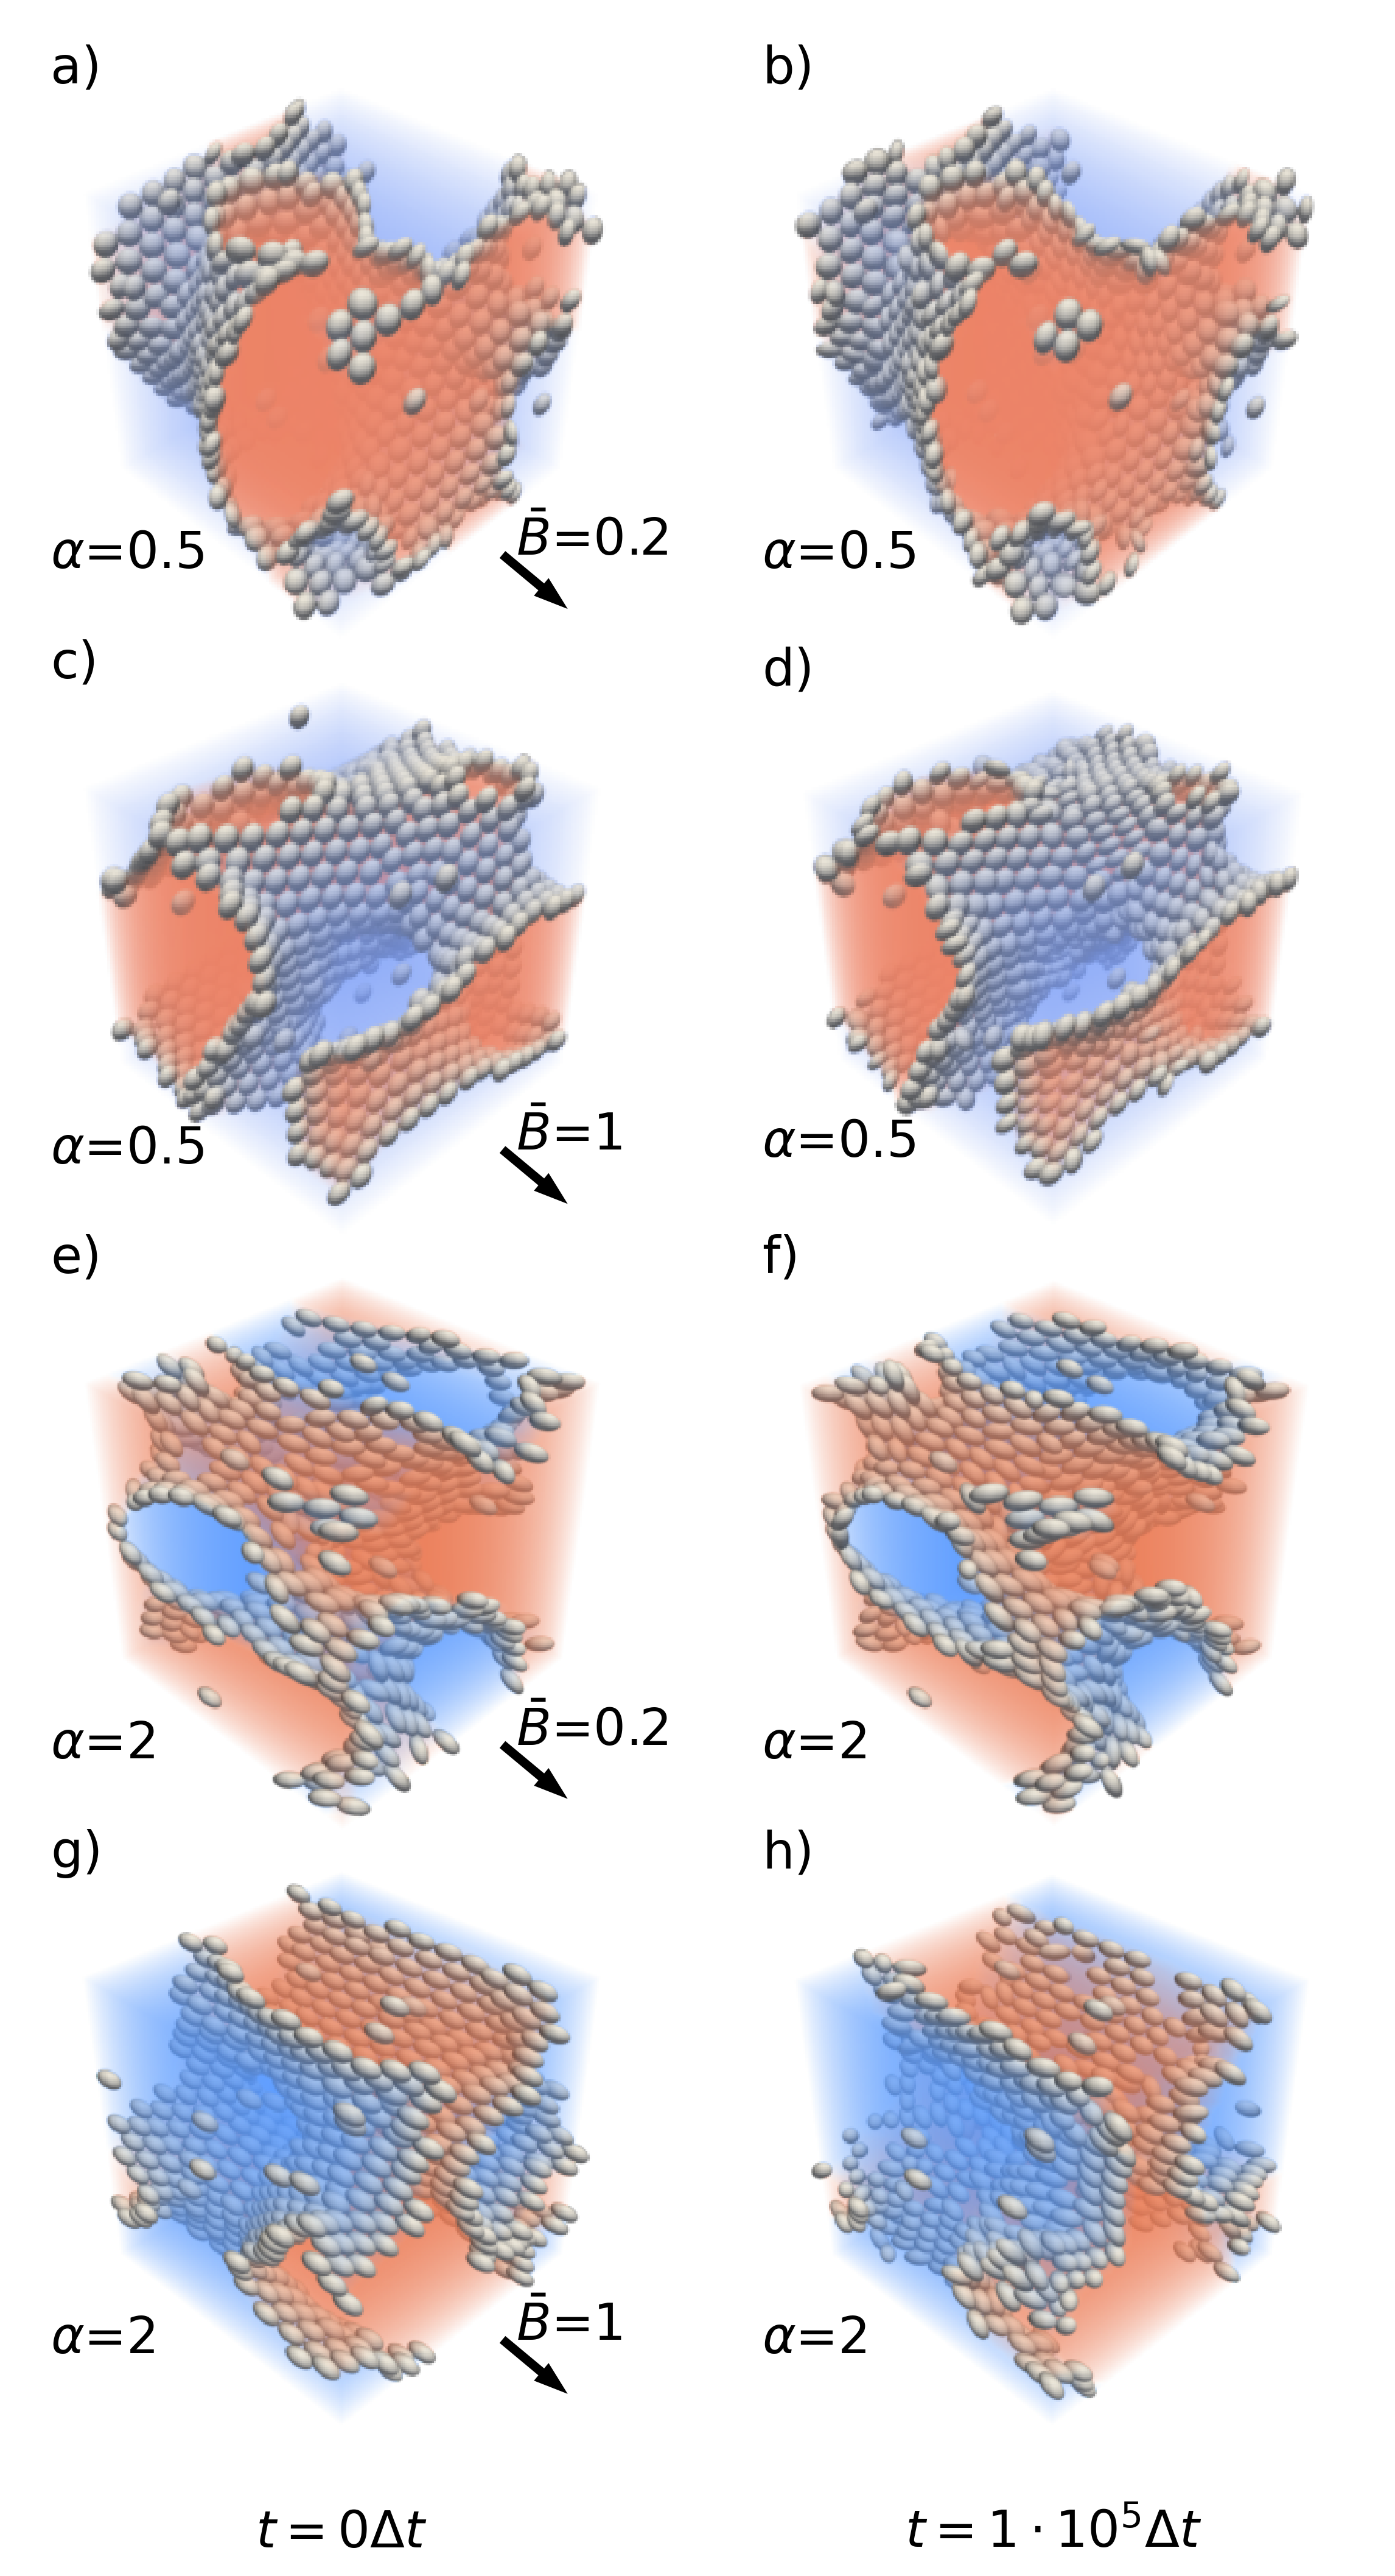
\includegraphics[scale=0.45]{../figures/results/paper2/microstructure_viz-field_down.png} 
\caption{Snapshots of bijels stabilized by prolate ellipsoids at 
         the initial and final time steps after the removal of an applied magnetic field. The top row corresponds to the case where 
         the field is reduced from \(\bar{B} = 0.2 \rightarrow 0.0\), and the bottom row from \(\bar{B} = 1.0 \rightarrow 0.0\)}
\label{fig:microstructure_viz-field_down}
\end{figure}

FIgure \ref{fig:microstructure_viz-field_down} shows that in 
both cases, the bulk microstructure remains effectively unchanged over the course of the simulation, highlighting the 
kinetic stability and arrested nature of the bijel once jamming has occurred.
However, closer inspection of the interfacial particle arrangement reveals subtle but important differences. In the 
\(\bar{B}: 0.2 \rightarrow 0.0\) case, the particles retain a degree of orientational order, although slight deviations 
from the field-aligned configuration begin to emerge. In contrast, for \(\bar{B}: 1.0 \rightarrow 0.0\), where the 
initial nematic order was stronger, the system exhibits more apparent disorganization by the final time step. This 
suggests that while the jammed interface resists large-scale rearrangement, there is a gradual relaxation of particle 
orientations in the absence of the aligning field. The extent of this relaxation appears to correlate with the initial 
alignment strength, indicating that systems formed under stronger magnetic fields exhibit greater reorientation when 
the field is removed. We probe the effect of these reorientations by calculating the time evolution of the domain size
and the corresponding nematic order parameter of the particles in Figure \ref{fig:domain_size-field_down}

\begin{figure} 
\centering 
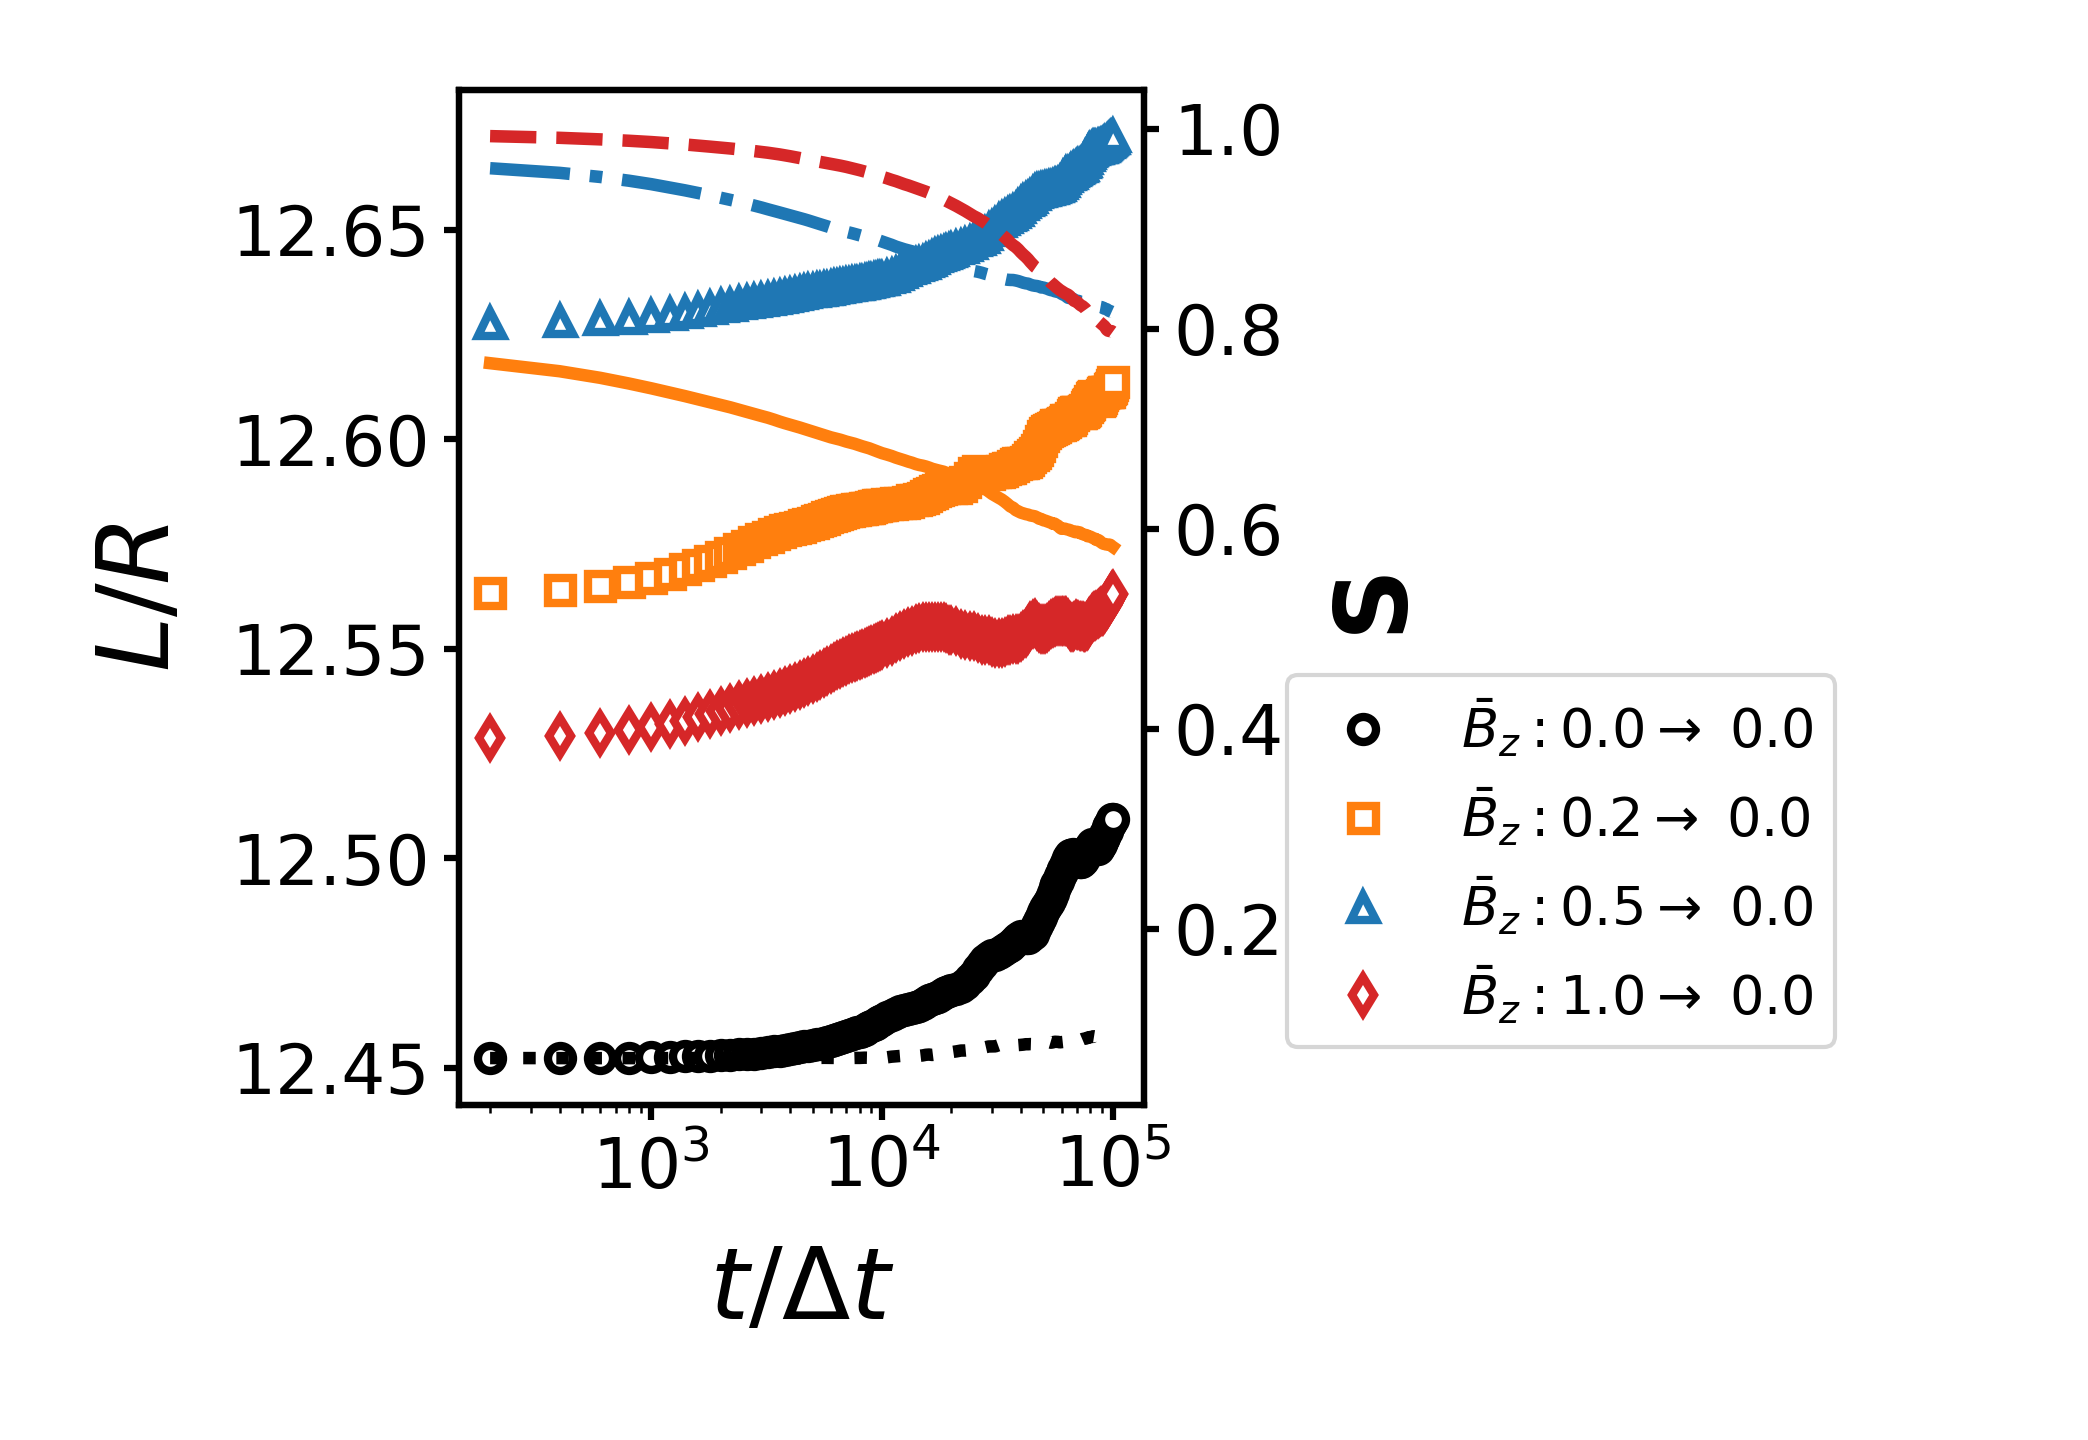
\includegraphics[scale=0.6]{../figures/results/paper2/domain_size-field_down.png} 
\caption{Plot of the spherically averaged domain size normalized with $R_p$ of the particle and the nematic order parameter of each bijel over time. 
         Each color represents bijel templates made with different field strengths $\bar{B}$. We show that there is domain coarsening when the field 
         is switched off, along with a reduction in the ordering of the particles.} 
\label{fig:domain_size-field_down} 
\end{figure}

Figure~\ref{fig:domain_size-field_down} presents the time evolution of the normalized domain size (\(L/R\)) and nematic 
order parameter (\(S\)) for bijels stabilized by oblate (left) and prolate (right) particles following the removal of an 
applied magnetic field. For all systems except oblate particle stabilized bijel with \(\bar{B}: 0.0 \rightarrow 0.0\), 
a modest degree of domain coarsening is observed. This slow, steady increase in domain size indicates that while the 
global microstructure remains largely intact, minor structural rearrangements may still occur post-stimulus, particularly 
at long timescales. This behavior is more prominent in prolate particle systems, suggesting that elongated particles 
may provide greater local flexibility for slight monolayer relaxation without disrupting the overall network.
A notable exception arises in the oblate \(\bar{B}: 0.0 \rightarrow 0.0\) case, which exhibits a sudden and pronounced 
increase in domain size at later times. This behavior is attributed not to gradual coarsening but to a domain coalescence 
event.

The nematic order parameter \(S\) for all field-removal scenarios demonstrates a consistent, order-dependent decrease over 
time. This trend suggests that in the absence of an aligning field, particles gradually relax from their field-induced 
configurations toward thermodynamically preferred orientations governed by interfacial capillary interactions. The 
magnitude of this decay correlates with the initial degree of ordering: systems formed under higher magnetic fields 
(\(\bar{B} = 0.5\) and \(1.0\)) show the most significant reduction in \(S\), reflecting a greater degree of reorientation.

These results reinforce the interpretation that bijel microstructure is resilient to field removal, with no meaningful 
reversal in domain architecture once jamming has occurred. However, the interfacial particle monolayer continues to evolve 
at the microscale, with orientation relaxation providing a residual mechanism for slow, local structural change. To determine 
whether this relaxation induces anisotropic coarsening, we next quantify the directional change in domain size and tortuosity 
using the relative change metric \(\Delta L = \frac{L_f - L_i}{L_i}\), applied separately to \(L_\perp\) and \(L_\parallel\). 
The same formulation is used to compute directional tortuosity changes, with results summarized in 
Figure~\ref{fig:domain_size_aniso-field_up}.

\begin{figure} 
\centering 
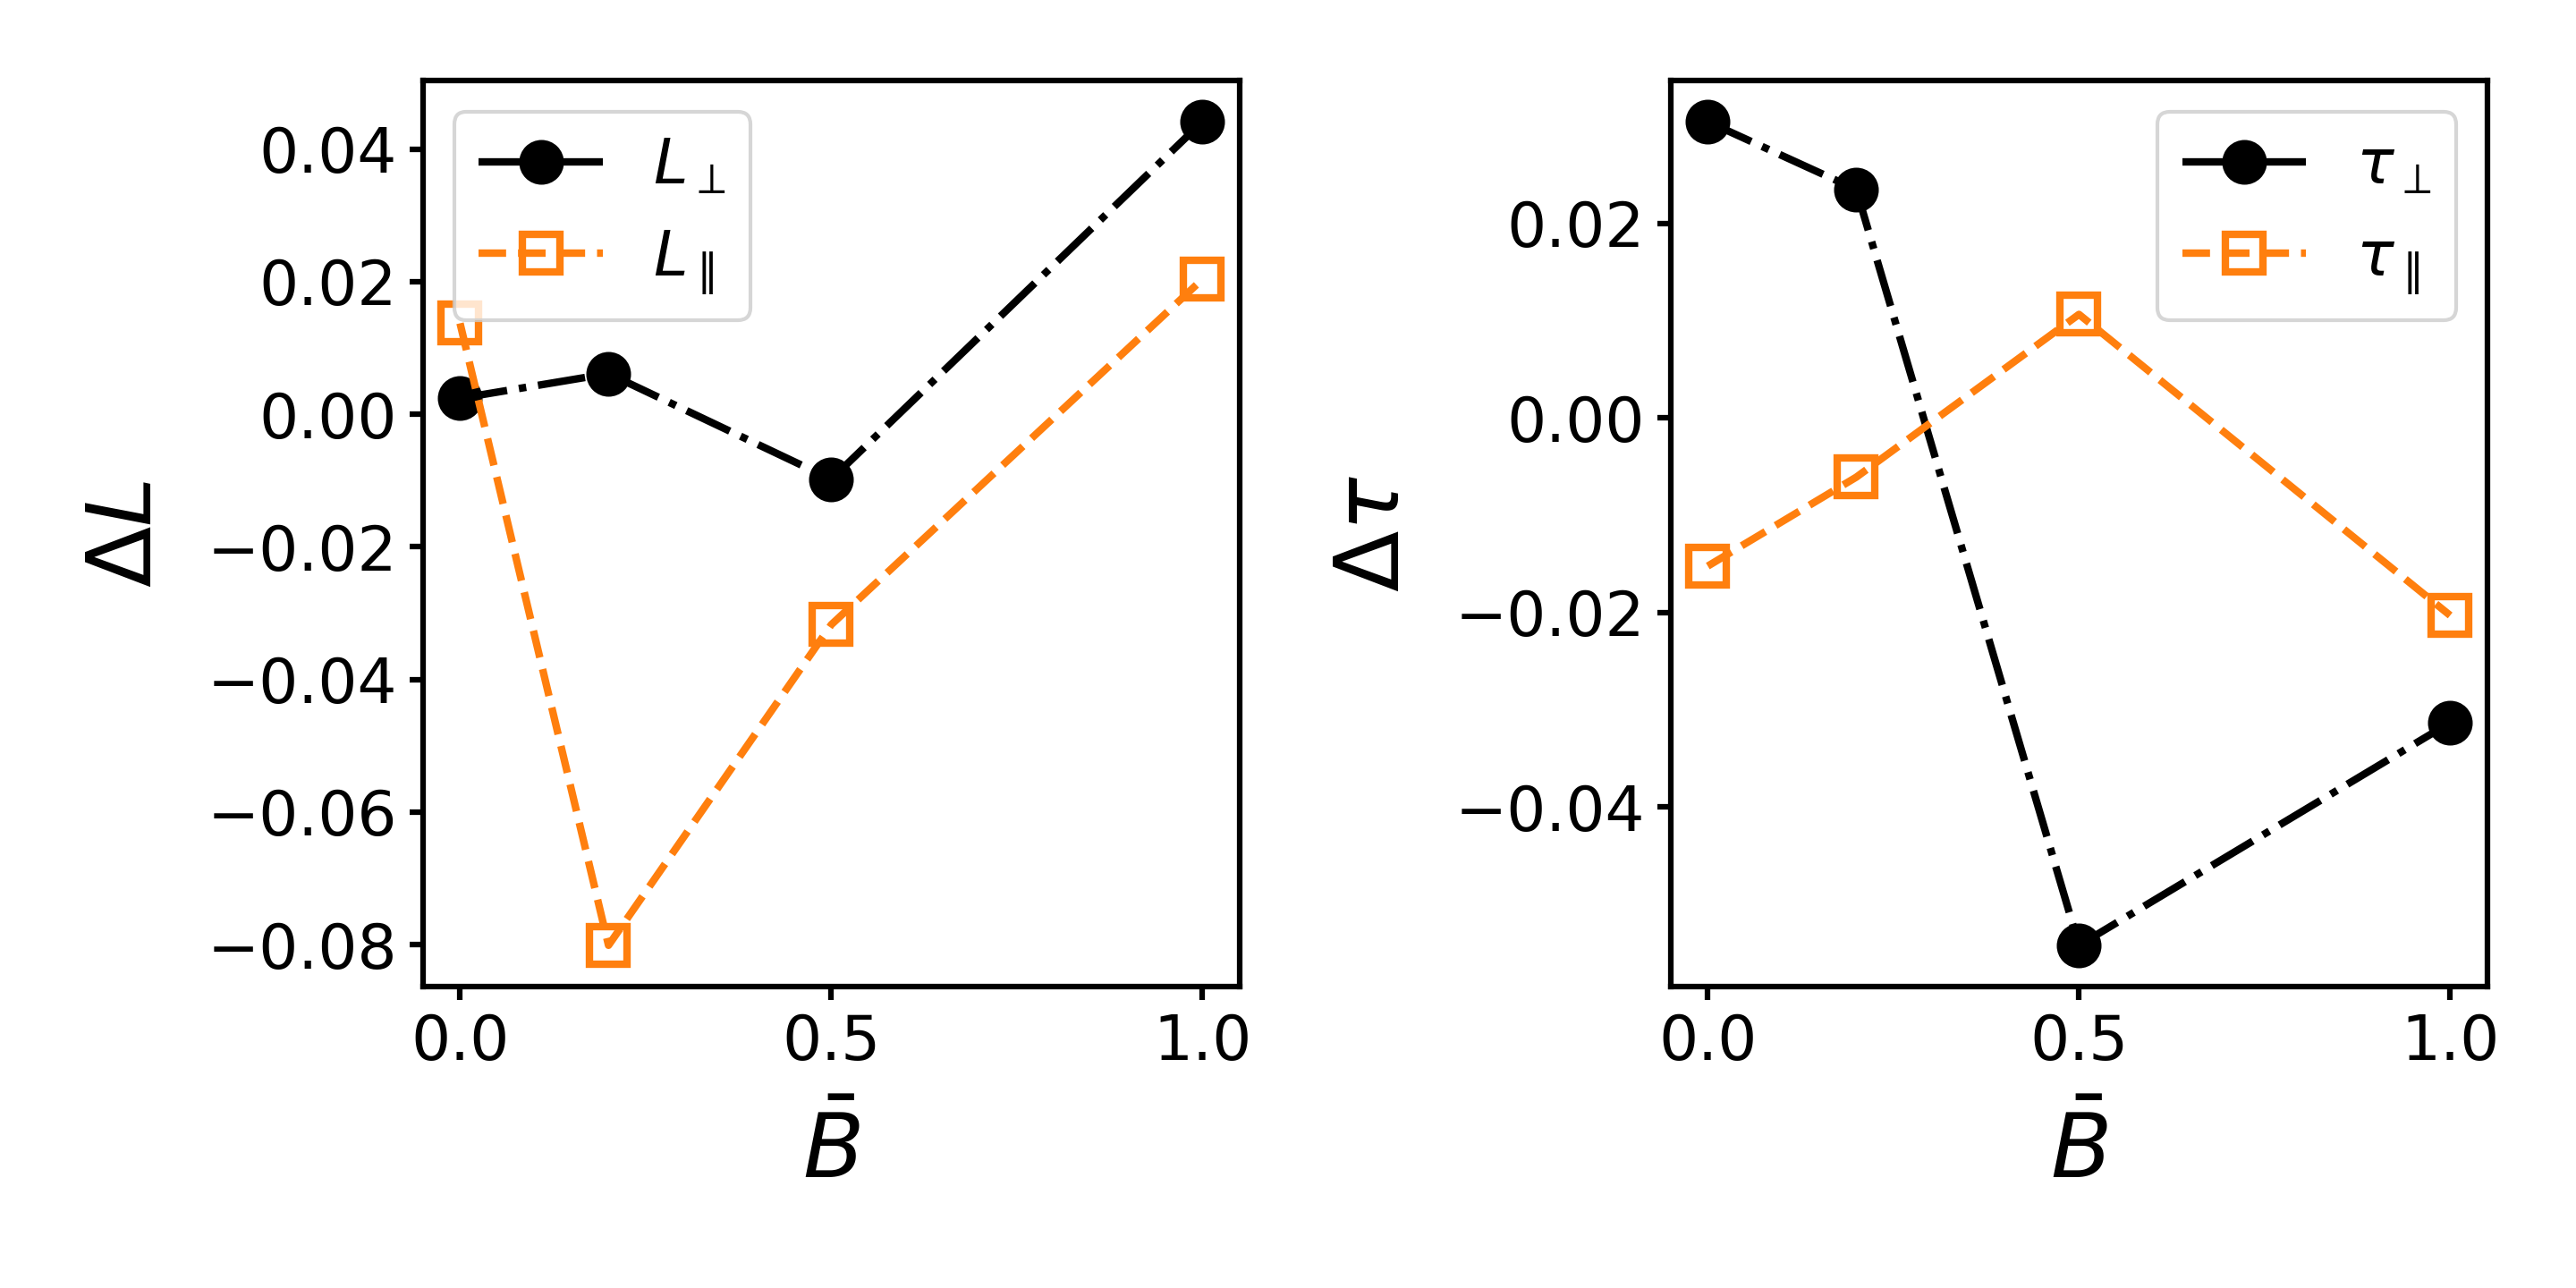
\includegraphics[scale = 0.6]{../figures/results/paper2/domain_size_aniso-field_down.png} 
\caption{Plots of the anisotropic structural response of bijels after the removal of 
         magnetic fields, by showing the relative change in directional domain size \((\Delta L)\) and tortuosity \((\Delta \tau)\) 
         as a function of \(\Delta \bar{B}\), the change in field strength from the templated to final state. Blue curves correspond 
         to bijels stabilized by oblate particles, and red curves to those stabilized by prolate particles.} 
\label{fig:domain_size_aniso-field_down} 
\end{figure}

Overall, only minor anisotropic changes in domain size and tortuosity are observed following field removal, with no consistent 
or monotonic dependence on \(\Delta \bar{B}\). This suggests that although particles may gradually relax from their field-induced 
alignment, the resulting structural rearrangements are subtle and largely isotropic at the microstructural scale. The small 
fluctuations observed in \(\Delta L\) and \(\Delta \tau\) likely reflect localized heterogeneities in the particle monolayer 
rather than coordinated, directional coarsening. These findings support the notion that once the magnetic field is removed, 
the dominant force acting on the particles is the interfacial capillary interaction, which seeks to minimize interfacial 
energy without preference for a particular direction.

Importantly, this contrasts with the structural response observed during the application of a magnetic field, where clear 
anisotropy emerged as a result of field-driven particle reorientation. Here, despite the monolayer initially being in an 
anisotropic, ordered state, the system exhibits no significant directional relaxation, underscoring the kinetic resilience 
of the jammed interface. Thus, the microstructural evolution following stimulus removal appears to be dominated by slow, 
isotropic relaxation rather than directional restructuring.To further understand the role of the capillary interactions on the 
particle monolayer, we examine the time evolution of the interface angle \(\langle \psi \rangle\). 

\begin{figure} 
\centering 
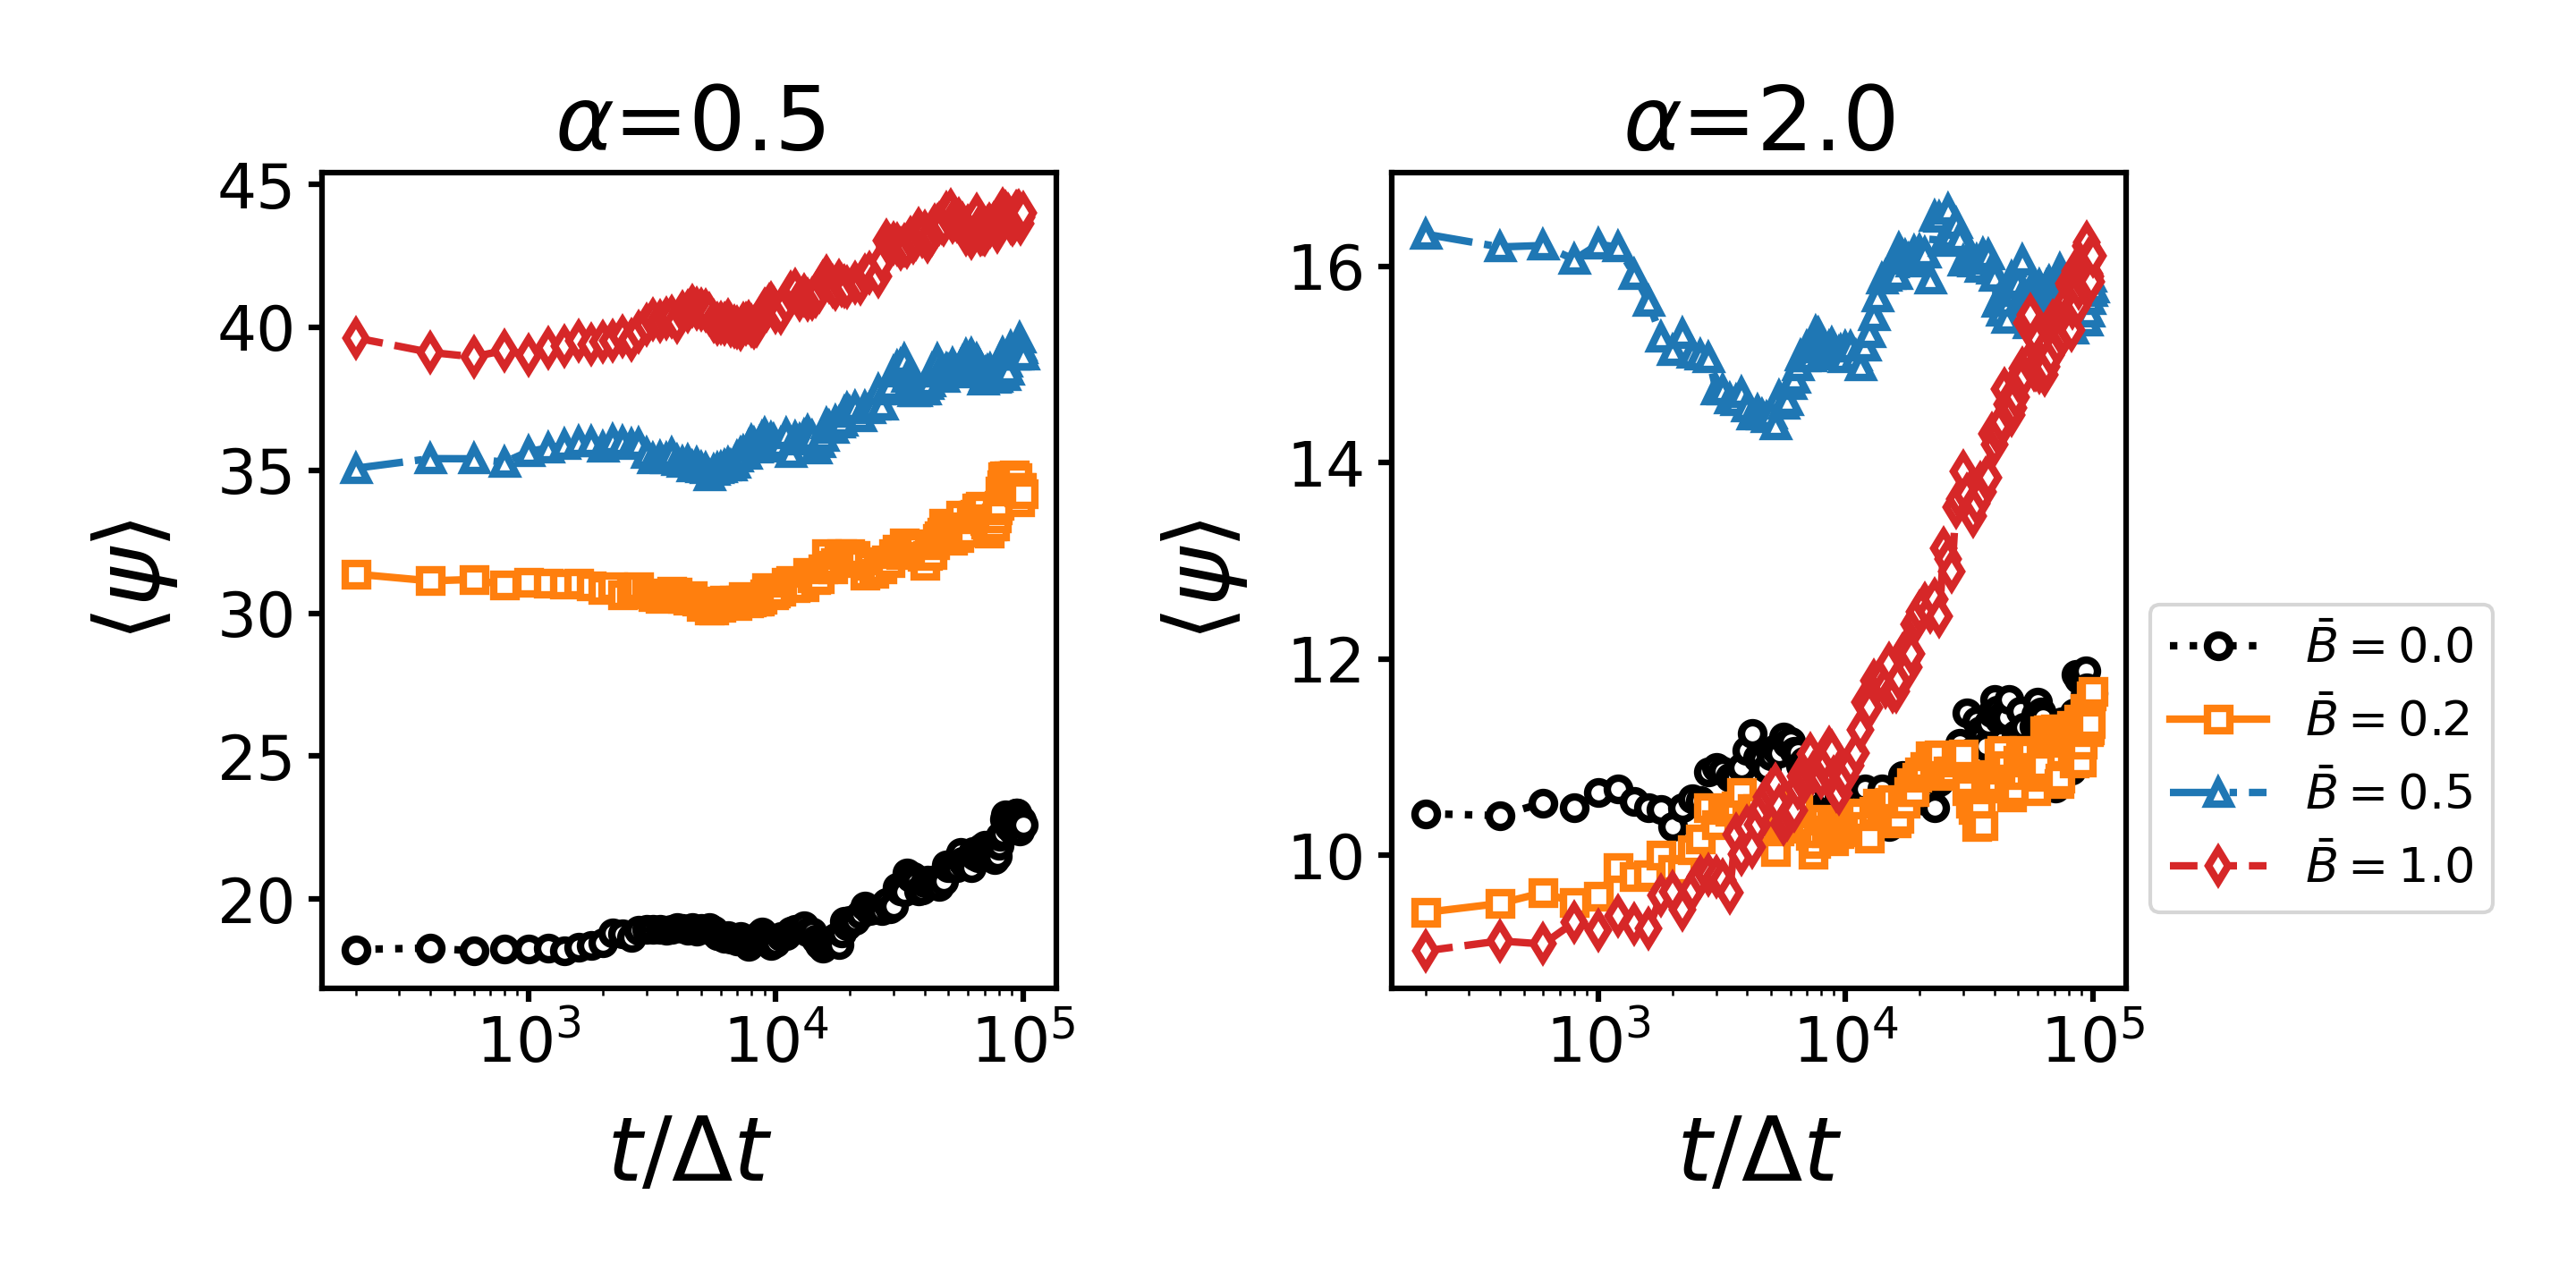
\includegraphics[scale=0.6]{../figures/results/paper2/psi-field_down.png} 
\caption{Plots of the average interfacial angle $\langle \psi \rangle$  plotted against time for bijels stabilized by oblate and prolate particles
         on the left and right plots respectively. They show slight increases in $\langle \psi \rangle$ over time indicating that the particles are
         slowly tilting out of the interface, inducing the domain coarsening observed.} 
\label{fig:interface_angle-field_down} 
\end{figure}

Figure \ref{fig:interface_angle-field_down} shows that the the rate and extent of angular relaxation appear relatively insensitive to the initial degree of 
order imposed by the templating field. For oblate particles, \(\langle \psi \rangle\) increases steadily regardless of initial alignment strength, indicating that 
even highly ordered monolayers do not retain their field-imposed orientation indefinitely. Similarly, for prolate particles, although the change in 
\(\langle \psi \rangle\) is smaller in magnitude, a comparable upward trend is evident.

These results suggest that the particle monolayer continues to evolve post field-removal, driven by interfacial forces seeking to minimize the total interfacial 
energy. However, since these angular adjustments do not lead to noticeable changes in the bulk microstructure it can be 
inferred that rotational relaxation alone is insufficient to trigger further domain coarsening once jamming has occurred. This supports the conclusion that 
structural irreversibility in these systems arises primarily from the kinetic constraints imposed by jamming, rather than any residual orientational stress 
within the particle layer.

\section{Conclusions}

In this work, we investigated how magnetic fields influence the structure and dynamics of bijels stabilized by magnetically responsive ellipsoidal particles. Motivated 
by the relevance of bijels in applications such as catalysis, membrane filtration, and drug delivery, we explored how external stimuli can enable in-situ control over 
microstructure in these systems. Using hybrid Lattice Boltzmann-Molecular Dynamics simulations, we characterized the structural response of formed bijels by investigating
the effect of applying a magnetic field and the initial microstructure on the structural response characterized. We first demonstrated that bijels subjected to increasing 
magnetic field strength exhibit hysteresis in its structural response, where the domain size increases with field application but does not revert upon field removal.

When investigating the effect of the application of magnetic fields, our results revealed that applying magnetic fields post-formation induces domain coarsening up to 5\%, with 
field-induced anisotropy dependent on particle shape. Oblate particles exhibited growth primarily in the perpendicular direction by up to 60\%, while prolate particles showed coarsening 
along the field direction up to 40\%, 
both accompanied by a decrease in tortuosity. These changes arise from particle reorientation to the field, followed by local unjamming and interfacial rearrangement before 
re-jamming occurs, as characterized using the average interface angle of the particles and the Steinhardt bond orientational order parameter.

Importantly, the extent of microstructural change scales with the difference in magnetic field strength before and after application. We found that particle alignment 
characterized via $\langle \psi \rangle$ and $\langle Q_6 \rangle$ governs domain evolution. Disordered particle layers exhibited strong field responses, while highly ordered 
templates showed minimal change, highlighting the importance of reordering on the structural response observed. In contrast, removing the magnetic field had little effect 
on bijel structure. Domain size and anisotropy remained largely unchanged, regardless of initial particle order. While minor relaxation in particle alignment was observed, 
capillary forces alone were insufficient to drive significant structural reorganization.

Together, these results identify modes of structural response that depend upon the initial ordering of particles at the interface. The first mechanism identified occurs with
disordered particle monolayers which upon application of a magnetic field, unjam facilitating domain coarsening before rejamming once the interface area matches the 
particle cross sectional area. The second mechanism occurs due to particle reorientation to the applied field when particles are nematically ordered but not ordered in the direction
of the magnetic field. 

While our simulations offer valuable insights into the tunability of bijels, they were limited to a single set of fluid and particle parameters. Future work could explore the 
effects of particle size, volume fraction, interparticle forces, and field orientation or gradients, all of which may unlock additional control over bijel structure.
Ultimately, this study establishes a foundation for stimuli-responsive bijels, showing how particle-level interactions and monolayer dynamics translate into controllable, 
application-relevant changes in material microstructure.